\chapter{Constraints on Neutrino Lifetime from SNO}
\label{ch:lifetime}

Analysis of the SNO data was instrumental in solving the SNP, and with the leading order dynamics of neutrinos established as the MSW effect, one can now explore the SNO data to constrain second order effects. 
Neutrino decay is one such effect, and was first explored as a possible explanation for the less-than-unity survival probability of electron flavor neutrinos \cite{bachall_stable}.
Even though neutrino decay is now known not to be the dominant effect behind the SNP, solar neutrinos make an excellent test beam for investigating neutrino decay.
Roughly speaking, this analysis will be searching for a deficit of neutrinos resulting from decay of neutrinos in flight from the Sun to the Earth.
As will be shown in the following sections, this produces an energy dependent distortion to the MSW survival probability curves that can be fit for in an analysis of SNO data.

The initial proposal to use solar neutrinos as a handle on neutrino lifetime explored a few models of neutrino decay and estimated that solar neutrinos could put the best limit on non-radiative neutrino decay~\cite{beacombell}.
The authors noted that the large uncertainty on the $^8$B flux as well as uncertainties in the neutrino mass and mixing parameters would be a limiting factor.
Relatively recent precise mixing parameters from KamLAND~\cite{kamland} and Daya Bay~\cite{dayabay} and improved theoretical predictions for the $^8$B flux~\cite{serenelli} mitigate this to some extent.
Further studies~\cite{berryman} using a simple disappearance model - where the neutrino decays into some non-active daughter(s) and the observable signal is an energy dependent distortion to the survival probability - were able to set respectable limits analyzing SNO~\cite{sno}, Super-Kamiokande~\cite{superk}, and Borexino~\cite{borexino} results.
Various constraints such as the eccentricity of the Earth's orbit allowed this limit to be improved~\cite{picoreti}. 
However, it was noted~\cite{berryman} that the published fits to the SNO data were not ideal for testing the simple disappearance model because the survival probabilities for electron neutrinos, $P_{ee}$, and the transition probability to other neutrino flavors, $P_{ea}$, were not treated as independent functions.
In a decaying scenario these probabilities are modified by an energy dependent form that does not preserve $P_{ee} + P_{ea} = 1$, which is a valid assumption in non-decaying scenarios and used in previous SNO analyses, so the authors concluded a better limit could be set with a dedicated fit.
This analysis aims to perform such a dedicated fit, specifically for the $\nu_2$ lifetime observed as an energy dependent modification to the standard MSW survival probability.

\section{Lifetime Model}
\label{lifetime_model}

The flux of a particular mass state $\nu_i$ could have some lifetime associated with it $\tau_i$ representing the decay of neutrinos of that mass state.
Since the actual neutrino masses are unknown the lifetime is often represented by an effective parameter $k_i$ scaled by the mass of the state
\begin{equation}
k_i = \frac{\tau_i}{m_i}.
\end{equation}
Since the Earth-Sun distance is so large compared to the solar radius any decay within the sun will be ignored. 
Therefore, using the formalism given in \Cref{ch:theory}, the detected flux $\psi_i$ of a neutrino mass state at earth can be given as 
\begin{equation}
\psi_i \approx  e^{-L_\odot / (E k_i)} \phi_i =  e^{-L_\odot / (E k_i)} \left| \braket{\nu_{m i}(V_e)}{\nu_e} \right|^2
\label{decay}
\end{equation}
where $L_\odot$ is the Earth-Sun distance (1~A.U.) and $E$ is the neutrino energy.
The survival probabilities for electron and muon/tau flavor neutrinos in a decaying scenario may then be calculated with appropriate factors from the PMNS matrix in the usual way,
\begin{equation}
\begin{array}{rcl}
P_{ee} & = & \sum_i \psi_i |U_{ie}|^2  \\
P_{ea} & = & \sum_i \psi_i |U_{i\mu}|^2 + \psi_i |U_{i\tau}|^2.
\end{array}
\label{survive}
\end{equation}

\subsection{Computing Survival Probabilities for $^8$B Neutrinos}

\label{montecarlo}

The three neutrino mass states each have a lifetime associated with them $k_i = \tau_i / m_i$, which are all physically interesting quantities to measure.
However, the characteristic energies of $^8$B neutrinos and the electron densities at the core of the Sun conspire to make the $^8$B flux a nearly pure flux of $\nu_2$.
The ultimate result of this is that an analysis of SNO data consisting of $^8$B neutrinos will be insensitive to $\nu_1$ or $\nu_3$ decay.
This is shown in \Cref{fig:frac_not_nu_2}, which shows the fraction of neutrinos (produced at electron densities consistent with $^8$B neutrinos) that exit the Sun as $\nu_2$, along with a typical $^8$B energy spectrum.
Weighting the former by the latter and averaging, one finds that less than $4\%$ of the detectable flux is not $\nu_2$
Therefore, for the purposes of this analysis, the lifetimes of mass state $\nu_1$ and $\nu_3$ are fixed at infinity as data taken by SNO for $^8$B neutrinos is nominally insensitive to $\nu_1$ or $\nu_3$ decay.

\begin{figure}
\centering
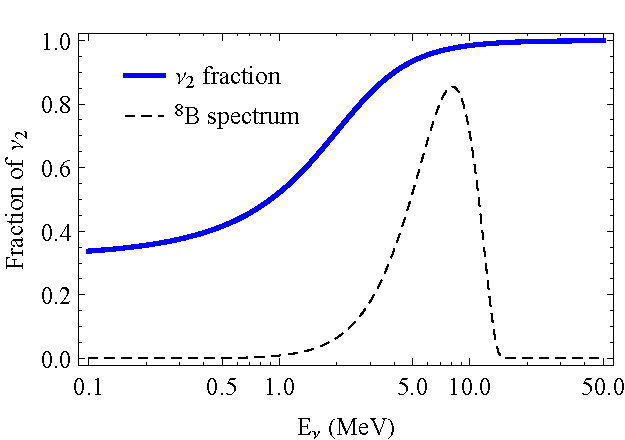
\includegraphics[width=0.75\columnwidth]{nu2_fraction}
\caption{
The fraction of $^8$B neutrinos that are $\nu_2$ upon exiting the Sun are shown here as a function of neutrino energy with a solid line, while the dashed line shows a typical $^8$B energy spectrum. 
This plot was created using central values for the neutrino mixing and standard solar model parameters. 
}
\label{fig:frac_not_nu_2}
\end{figure}

$^8$B solar neutrinos are produced in a continuous region of the Sun, which samples a large range of electron densities.
This variation in electron density must be propagated into the modeled survival probability curves.
\Cref{fig:core_density} shows the variation in the survival probability of neutrinos from the core of the Sun to a tenth of the solar radius.
$^8$B neutrinos are primarily produced at intermediate radii.

\begin{figure}
\centering
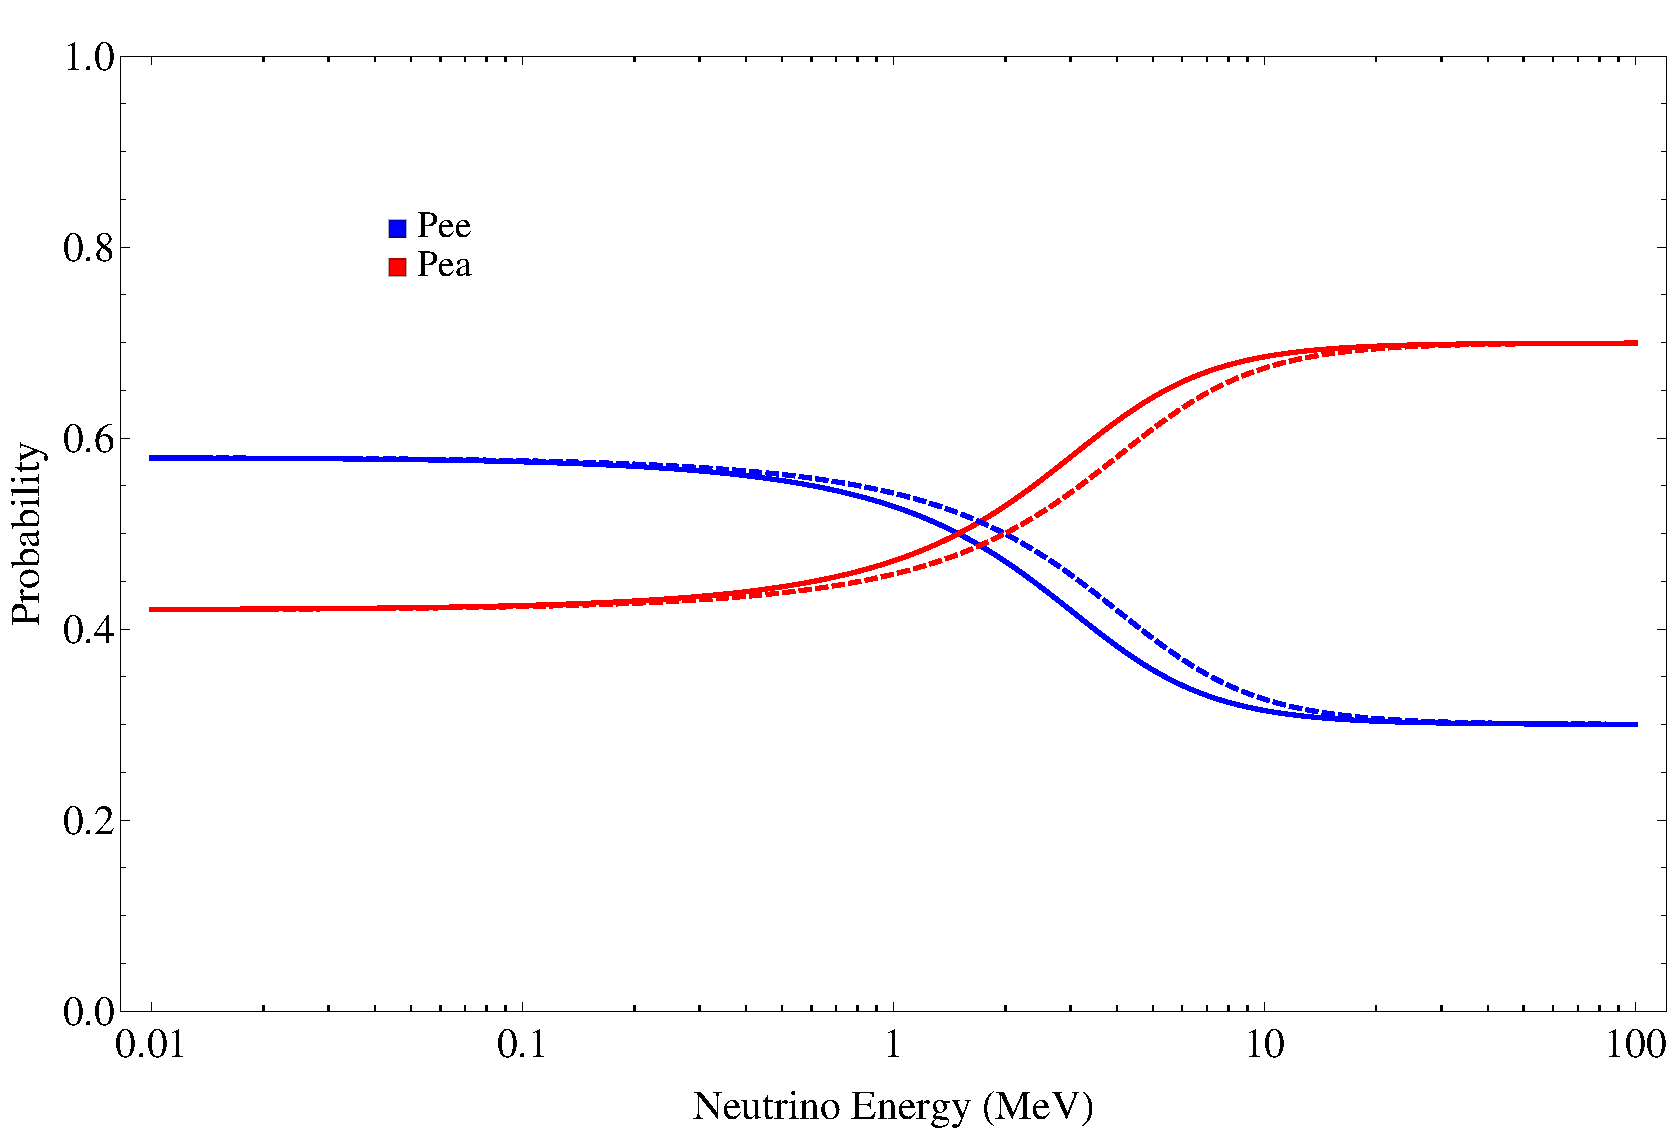
\includegraphics[width=0.75\columnwidth]{survival_core}
\caption{The solid lines here represent the MSW survival probability curves for neutrinos at the center of the solar core, with neutrinos produced a $0.1R_{\odot}$ in dashed lines. Most $^8$B neutrinos come from intermediate densities.}
\label{fig:core_density}
\end{figure}

However, because a numerical method must be used to compute the MSW effect in a three neutrino scenario, one cannot simply integrate over this variation in electron density to arrive at the average survival probability. 
To calculate the survival probability of a $^8$B neutrino numerically for a particular neutrino energy value, a MC method is used:
\begin{enumerate}
\item Generate an ensemble of radial positions sampled from the SSM radial distribution for $^8$B neutrino flux.
\item Use the SSM electron density distribution to find the electron densities for this ensemble.
\item For each electron density, numerically diagonalize the Hamiltonian $H_{MSW}$ from \Cref{eq:msw} in the flavor basis using TMatrixDEigen from ROOT~\cite{root}.
\item These eigenvectors are  $\ket{\nu_{mi}(V_e)}$, and their projection onto $\ket{\nu_e}$ is trivial in the flavor basis.
\item The quantity \Cref{decay} is calculated using these projections for a particular values of $k_i$.
\item Survival probabilities are calculated with \Cref{survive} and averaged across the ensemble.
\end{enumerate} 

This process can be executed for any neutrino energy, producing survival probability curves for neutrinos produced in regions consistent with $^8$B neutrinos.
Example survival/oscillation probability curves produced this way for different values of $k_2$ are shown in \Cref{fig:model}.

\begin{figure}
\centering
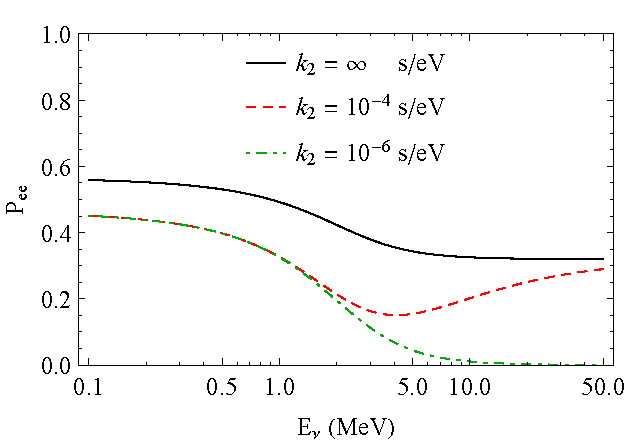
\includegraphics[width=0.75\columnwidth]{decay_msw_pee_theory}
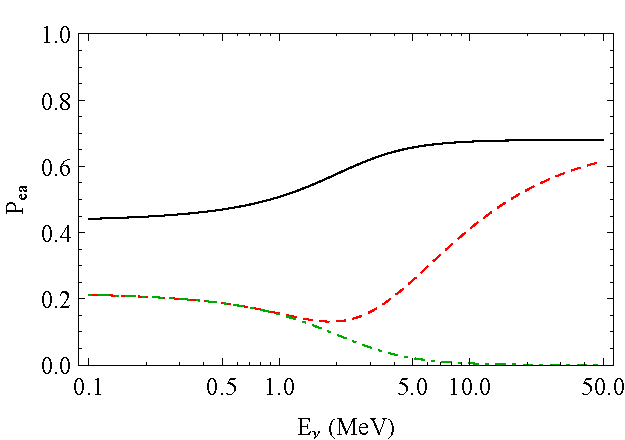
\includegraphics[width=0.75\columnwidth]{decay_msw_pea_theory}
\caption{
Shown here in dashed lines are survival probability of
electron neutrinos $P_{ee}$ and the oscillation probability $P_{ea}$ for
various values of mass state $\nu_2$ lifetime ($k_2$), demonstrating the
energy-dependent distortion being modeled. Both $k_1$ and $k_2$ are fixed
to infinity in these plots. Existing limits are near $k_2 = 10^{-4}$ s/eV.
The solid line shows the survival probability with no neutrino
decay ($k_2 = \infty$).
}
\label{fig:model}
\end{figure}

\subsection{Parameters}
\label{parameters}

The parameters of the neutrino lifetime model beyond the quantity of interest, the lifetime $k_2$ of mass state $\nu_2$, are discussed in the following sections.
In all cases, fundamental constants are taken from the Particle Data Group (PDG)~\cite{pdg}.

\subsubsection{Neutrino Mixing}
Neutrino mixing parameters taken from KamLAND~\cite{kamland} and Daya Bay~\cite{dayabay} are reproduced in \Cref{tbl:mixing_params}. 
Parameters from KamLAND and Daya Bay were used to avoid bias from using SNO results in this analysis.
As these measurements were done at Earth with neutrinos produced on Earth, they are expected to be uncorrelated with effects of $\nu_2$ decay.
The current limit on $k_2$ constrains it to be greater than $\approx7\times10^{-4}$~\cite{picoreti}, which means at length scales comparable to the diameter of the earth the maximum flux lost by $\nu_2$ decay for a $10$ MeV neutrino is given by
$1-e^{-2R_{earth}/(E k_2)} \approx 6\times10^{-6}$,
which would have negligible impact on values quoted for mixing parameters.

\begin{table}
\centering
\begin{tabular}{c|c|c}
Parameter & Value & Ref \\ \hline
$ \Delta m ^2 _{21} $ & $7.58^{+0.14}_{-0.13}(stat)^{+0.15}_{-0.15}(syst) \times 10^{-5}$~eV$^2$ & \cite{kamland} \\ \hline
$ \tan^2 \theta_{12} $ & $0.56^{+0.10}_{-0.07}(stat)^{+0.10}_{-0.06}(syst) $ & \cite{kamland} \\ \hline
$ |\Delta m ^2 _{32}| $ & $2.45\pm0.06(stat)\pm0.06(syst) \times 10^{-3}$~ev$^2$ & \cite{dayabay} \\ \hline
$ \sin^2 2\theta_{13} $ & $0.0841\pm0.0072(stat)\pm0.0019(syst)$ & \cite{dayabay} \\ \hline
$ \sin^2 \theta_{23} $ & $0.5^{+0.058}_{-0.062}$ & \cite{superkth23} \\ 
\end{tabular}
\caption{
\label{tbl:mixing_params}
Reproduced here are the mixing parameters used in this analysis taken from Daya Bay~\cite{dayabay}, Super-Kamiokande~\cite{superkth23}, and KamLAND~\cite{kamland} results.
}
\end{table}

\subsubsection{Standard Solar Model}

The model implemented here uses the distribution of electron density and distribution of neutrino fluxes calculated in the BS05(OP) Standard Solar Model (SSM)~\cite{bs05op}, which are reproduced in \Cref{fig:ssm}. 
Uncertainties in these values are not quoted in the original source and are therefore not considered here.
These predictions are expected to be unaffected by potential $\nu_2$ decay as they are not constrained with neutrino flux measurements.

\begin{figure}
\centering
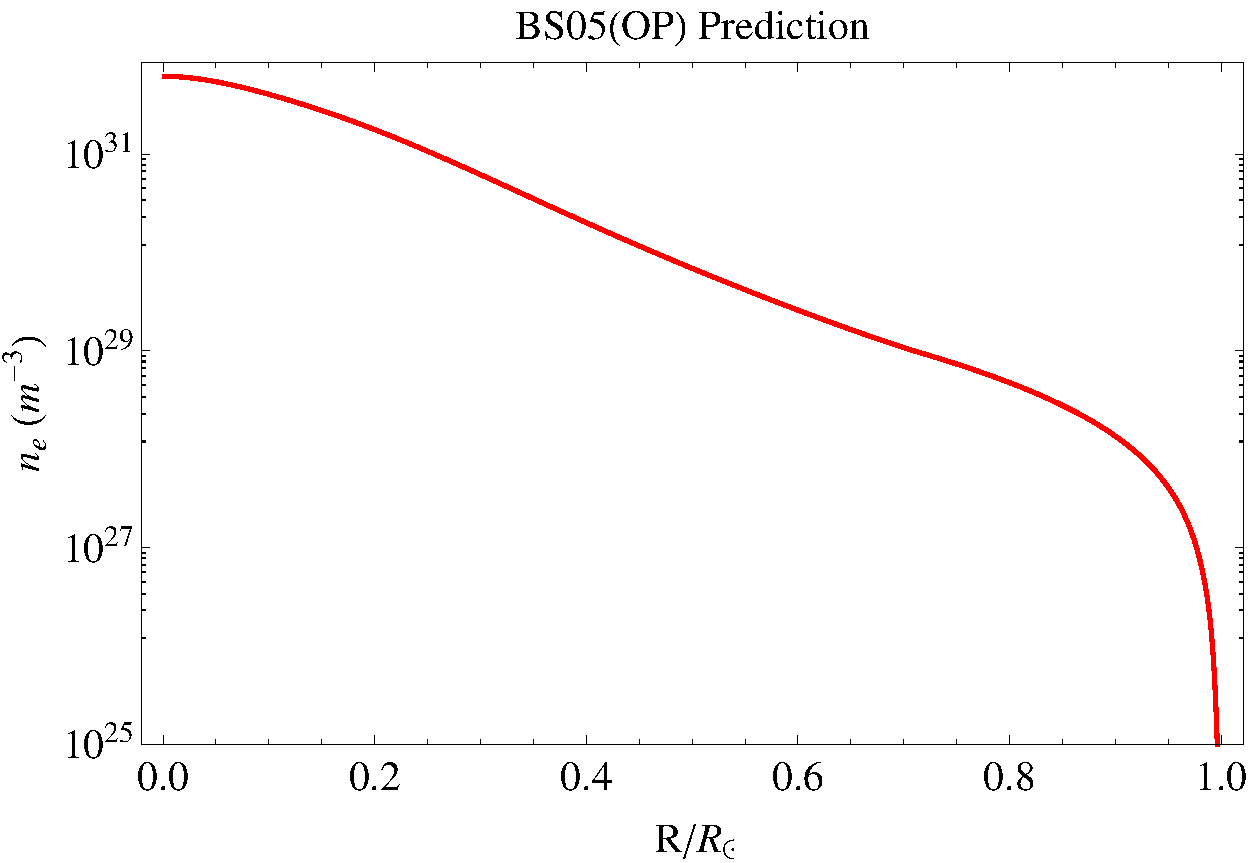
\includegraphics[width=0.48\columnwidth]{ssm_ne}
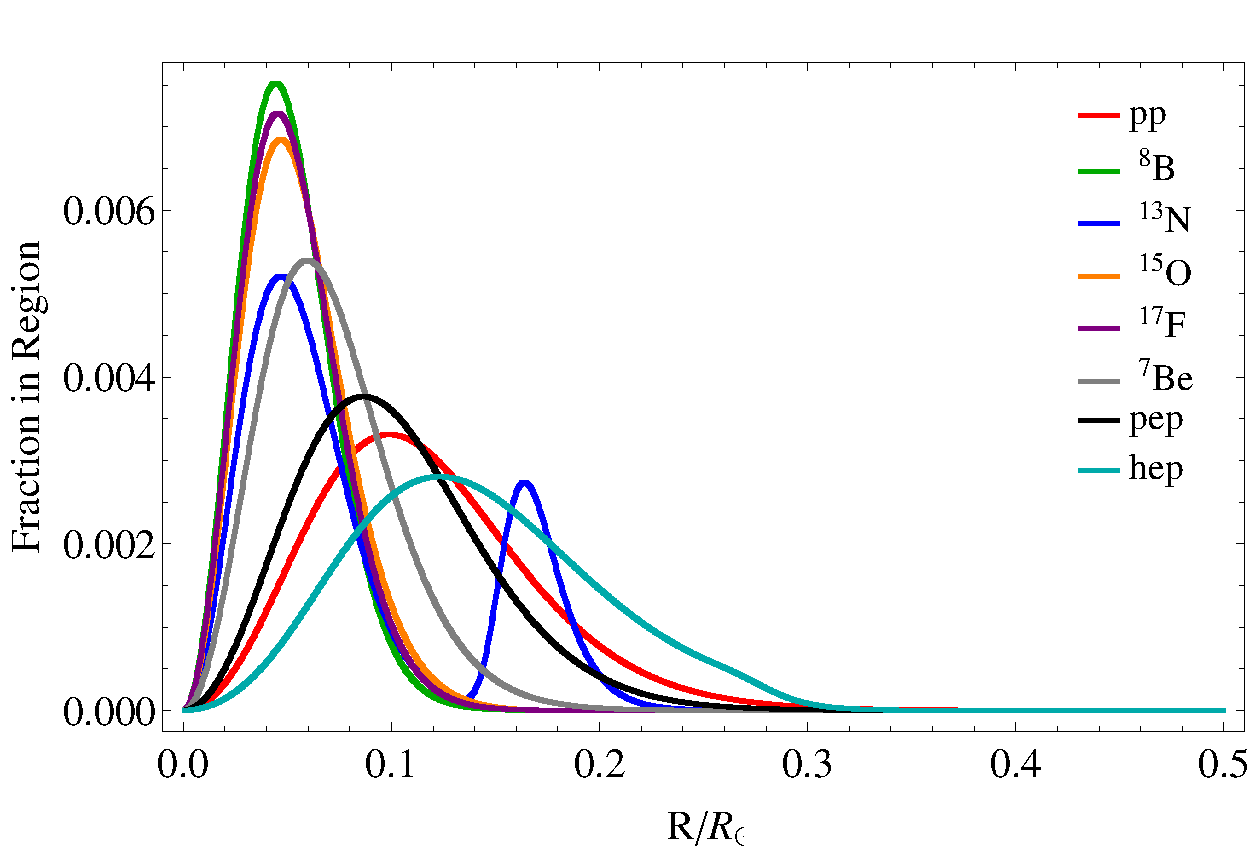
\includegraphics[width=0.48\columnwidth]{ssm_nu_region}
\caption{
The electron density in the Sun as a function of radius and the fraction of the neutrino flux produced in a radial region as a function of radius for the different neutrino fluxes. Only the $^8$B flux is relevant for this data. From the BS05(OP) SSM~\cite{bs05op}.
}
\label{fig:ssm}
\end{figure}

\subsubsection{$^8$B Flux}

As earth bound measurements of the solar neutrino flux would be biased by neutrino decay, a theoretical prediction for the $^8$B flux is required.
Serenelli's most recent prediction yields a $^8$B flux of $5.88\times10^{6}$~cm$^{-2}$s$^{-1}$ with $11\%$ uncertainty~\cite{serenelli}, which is used as a prior in this fit.
For reference the flux from BS05(OP)~\cite{bs05op} traditionally used in SNO analyses is $5.69\times10^6$~cm$^{-2}$s$^{-1}$.
See \Cref{strategy} for further discussion of how the flux is handled.

\section{Fit Implementation}
\label{fit_impl}

For this analysis, I have built off the existing QSigEx code \cite{plthesis}, which properly handled nuisance parameters, PDF generation, data binning, and likelihood function implementation for the published 3-phase analysis of SNO data \cite{3phase}.
This package was modified to use the model described in \Cref{lifetime_model} instead of polynomials used in previous analyses.
The following sections conceptually describe how to analyze SNO data, the implementation of such an analysis in QSigEx, and the work that was necessary to implement the neutrino lifetime model in this framework.
Since QSigEx was previously vetted for SNO fits, a demonstration that the updated code produces the same results as previous analyses is given in \Cref{qsigex_validation}.

\subsection{Extended Log Likelihood}

The physical observables determined from vertex reconstruction can be used to statistically sort events into different classes of interactions.
Here the statistical sorting is done with a maximum likelihood fit: QSigEx finds the model parameters best describing the data by varying these parameters and maximizing the Poisson likelihood of the observed data.
This is done by minimizing the well known form of the log likelihood:
\begin{equation}
    \mathcal{L} = -\nu + \sum_{i=1}^{n_{events}} \log \left[ \nu f(\vec{x_i}) \right],
\end{equation}
where $\nu$ is a Poisson mean number of observed events and $f(\vec{x_i})$ is a PDF evaluated $\vec{x_i}$, which is a vector of quantities describing event $i$.
In the case of many classes of events with Poission parameters $\nu_j$ decribed by PDFs $f_j$ this log likelihood this can be written as:
\begin{equation}
    \mathcal{L} = -\sum_{j=1}^{n_{classes}} \nu_j + \sum_{i=1}^{n_{events}} \log \left[ \sum_{j=1}^{n_{classes}} \nu_j f_j(\vec{x_i}) \right].
\end{equation}
In a typical SNO analysis, each type of signal or background for each phase is treated as a separate event class.
When the rates of these classes are expected to be correlated across phases, the Poisson parameter for those classes are constrained to be the same value.
In this way one can simultaneously fit to all three phases of SNO data in a self consistent manner.

\subsection{Analyzing SNO Data}
\label{sec:sno_observables}

In SNO the observable quantities of choice are:
\begin{enumerate}
    \item Energy - the estimated deposited energy assuming Cherenkov light from an electron. Necessary for recovering spectral information for solar neutrinos and disentangling low energy backgrounds from higher energy solar neutrinos.
    \item Radius - the volume weighted radius of the event estimated from reconstruction. Useful for distinguishing neutrino events, which are isotropic within the detector from intrinsic radioactivity, which is maximal at higher radii due to a very successful background reduction campaign within the AV.
    \item Isotropy - the $\beta_{14}$ parameter based on Legendre polynomials giving a direction independent measure of isotropy of hits. Can distinguish between multi site events (multiple gammas scattering multiple electrons - NC) and single electrons (CC, ES). Also capable of discriminating between physics events (Cherenkov hit topology) and instrumental backgrounds.
    \item Direction - the cosine of the angle between the reconstructed event direction and the direction to the Sun at the time of the event. Identifies ES electrons, which are highly correlated with the solar direction, and provides some discrimination for CC electrons.
\end{enumerate}
These observables were chosen to maximize separation between different types of physics interactions (NC, CC, ES) and of physics, backgrounds, and instrumentals. 
To properly take into account correlations between these parameters, 4D PDFs were used instead of four separate 1D PDFs.
A notable exception is the inclusion of Phase III data, where the NCDs present in the target volume significantly complicated photon propagation, and made $\beta_{14}$ a less reliable metric than in Phases I and II.
For Phase III, 3D PDFs in energy, radius, and direction were used.

The likelihood fit determines the relative contribution of each event class necessary to best match the observed data.
To do this, the fit needs the 4D PDF for each type of event, and these PDFs were generated using a MC method.
SNOMAN \cite{sno_nim} was a FORTRAN simulation package developed by SNO that was adjusted to reproduce calibration data taken with the detector.
The reconstruction algorithms used on raw data were applied to the simulation results of SNOMAN for known classes of interactions to produce the PDFs used in analysis.

Most PDFs are constructed by directly binning simulated data produced by SNOMAN.
The physics encoded by the neutrino survival probabilities is included by reweighting solar neutrino events from SNOMAN while building the PDFs for solar signals.
For the radioactivity of the PMT glass, only tails of this high-rate background fall within the ROI, and it was impractical to simulate a sufficient number of interactions to produce reliable PDFs.
In this case, analytical forms were used instead, and the parameters controlling these analytical forms were estimated from the data and treated as systematic uncertainties.

\subsection{Building Solar PDFs}

There are two options for handling the neutrino energy dependence in such a fit:
\begin{itemize}
\item Binned neutrino energy fits where where the neutrino MC is binned into $N$ PDFs by neutrino energy prior to the fit, and the average value of the survival probability across that entire bin is applied to each of the $N$ PDFs when stepping though the minimization.
\item Unbinned neutrino energy fits where each of the $M >> N$ neutrino MC events are reweighted by the value of the survival probability at their exact energy when stepping through the minimization to build the neutrino PDFs.
\end{itemize}
Clearly the binned fit will perform more poorly as an average value of the survival probability across a neutrino energy bin is applied to all neutrinos in that bin, however, this method is much faster, being computationally far simpler than rebuilding the PDFs at each minimization step. 
For polynomial fits of previous SNO analyses, this poorer performance was not significant and allowed the minimization algorithm to benefit from the increased speed.
Unfortunately preliminary tests of the binned fit had very poor results regarding capturing the shape of the lifetime model survival probabilities.
Because of this, an unbinned neutrino energy fit was adopted.

\subsection{Detector Systematic Effects}
\label{systematics} 

Systematic uncertainties are treated in three distinct ways.
\begin{enumerate}
\item Each of the observables has many systematic parameters associated with it representing possible discrepancies between simulated and real data. These uncertainties are best constrained with the data itself, and most likely central values along with their uncertainties are determined with an initial brute-force iterative scan of each parameter while maximizing the likelihood of the data. These parameters are then held fixed during the central fit, and uncertainties are propagated with a shift-and-refit method.
\item Other uncertainties are best constrained with in-situ and ex-situ measurements and not highly correlated with neutrino parameters. These are also held fixed during the central fit, and uncertainties are propagated with a shift-and-refit method.
\item Finally, the NCD neutron capture efficiency, which is strongly correlated with measurements of the neutrino flux, is allowed to float in the fit to avoid biasing neutrino results.
\end{enumerate}

The procedure for determining the central values and uncertainties of scanned parameters is as follows:
\begin{enumerate}
\item A parameter is scanned around its current best guess with other systematics held at their best guess.
\item At each point in the scan, the minimization algorithm is run, finding the minimum negative log likelihood value.
\item This produces a negative log likelihood profile as a function of the parameter of interest.
\item An asymmetric gaussian is fit to the profile of the negative log likeihood to determine the central and upper/lower uncertainties for the parameter.
\item The best guess for that parameter is updated to the central value of that fit.
\item The next parameter is considered at step 1 until all parameters have been scanned.
\item If any parameter central value has shifted relative to the previous iteration, the algorithm repeats until stable minima are found.
\end{enumerate}

The shift-and-refit algorithm is intended to stochastically marginalize over the bulk of the systematic uncertainties. 
This was done for two reasons.
First, variation in many of the systematics result in events moving between bins and discontinuities in the likelihood space, which interfere with minimization algorithms.
Stochastic methods are not susceptible to such discontinuities.
Second, there are very many systematic uncertainties, and floating them all would result in an intractably large parameter space.
Therefore those systematic uncertainties not strongly correlated with neutrino parameters are treated with the following shift-and-refit procedure to propagate their uncertainties into the final results:
\begin{enumerate}
    \item A million sets of randomly sampled systematic parameters are produced by sampling asymmetric Gaussian distributions of parameter uncertainties. These distributions are either known from independent analyses or determined by initial scans of the dataset. 
    \item For each set of parameters, the fit is minimized again and the central value of each floated parameter is recorded.
    \item This produces a distribution of shift-and-refit values for each floated parameter, which represent the systematic uncertainties on these parameters.
\end{enumerate}

If the shift-and-refit distributions are approximately normal, the upper and lower RMS represents the upper and lower systematic uncertainty. 
This applies to most floated parameters, but notably not to $k_2$, which was shown to have highly asymmetric errors. 
In the case of $k_2$, an assumption is made that the shape of the likelihood space does not change with variations in the central value of $k_2$ but rather the minimum simply shifts.
Taking this assumption, the likelihood profile for $k_2$ obtained with systematics fixed to their central values can be shifted by each shift in the shift-and-refit distribution for $k_2$ and averaged to obtain a likelihood profile including systematic uncertainties.

\subsection{Fit Strategy}
\label{strategy}
Ideally all neutrino parameters would be floated with priors in this analysis. 
In practice it has been observed that the fit does not converge with both the $^8$B flux and lifetime parameter floated unless there is a very strong external constraint on the flux.
This is most easily understood by considering the signature of neutrino decay: a disappearance of neutrino flux.
Manifestly neutrino decay and the total flux will be highly correlated, however, the energy dependent signature of neutrino decay allows these effects to be disentangled to some extent.
Previous SNO analyses searching for oscillation to sterile neutrinos \cite{plthesis} have encountered a similar issues and opted for a strategy of finding a preferred $^8$B flux in some reduced parameter space, performing further fits and statistical studies with the flux fixed, and finally incorporating uncertainty from flux variations as a final step.
In this analysis since there is only one model parameter of interest, $k_2$, a strategy of scanning $k_2$ manually while floating all other parameters seems to be ideal. 
With that in mind, the fit strategy is:
\begin{enumerate}
\item Perform a scan over $k_2$ minimizing floated parameters at each point producing a likelihood profile. For data fits this can be done along with the other scanned nuisance parameters.
\item At the best, use MINOS fit errors (implicitly with $k_2$ fixed) as the total uncertainty on all parameters except the highly correlated $k_2$ and $^8$B flux.
\item For $k_2$ find the total uncertainty by at the point where change in negative log likelihood profile with respect to the minimum is $0.5$.
\item For the total uncertainty on $^8$B flux this value is scanned the same way as $k_2$ to properly account for the correlations in with $k_2$.
\item Combine with these uncertainties on $k_2$ and the $^8$B flux additional shift and refit uncertainties from scanned nuisance parameters.
\end{enumerate}

\section{Ensemble Testing}
\label{ensemble_tests}

To demonstrate that the fit described above is unbiased and correctly estimates errors on the fitted parameters, statistical tests were done on an ensemble of fake datasets.
These fake datasets are generated with known parameters, and the results of the fit are compared to these known quantities to demonstrate there is no systematic bias in parameter estimation.
This is done by ensuring a distribution of biases has a mean consistent with zero.
Further, statistical fluctuations resulting in biases in individual fits are compared to the errors estimated by the minimization algorithm by computing pull distributions for each parameter. 
A pull distribution with a width of 1 indicates the fit is properly estimating errors.
Finally the relative uncertainty of each parameter shows the sensitivity to each of the floated parameters.
These figures of merit are defined as:
\begin{equation}
Pull = \frac{Fit\,\,\,value - Actual\,\,\,value}{Fit\,\,\,uncertainty}
\end{equation}
\begin{equation}
Bias = \frac{Fit\,\,\,value - Actual\,\,\,value}{Actual\,\,\,value}
\end{equation}
\begin{equation}
Relative\,\,\,uncertainty = \frac{Fit\,\,\,uncertainty}{Actual\,\,\,value} \times 100\%
\end{equation}

This testing is done in three stages, starting with only solar neutrino events, and then with progressively more backgrounds added in order of importance.
For each stage of testing a plot showing the mean and width (as error bars) of the bias and pull distributions are produced.
Plots of the pull show the expected fluctuations of the mean ($1/\sqrt{n_{samples}}$) in dashed lines with the expected mean ($1 - 1/(4(n_{samples}-1))$) and fluctuation of the standard deviation ($1/\sqrt{n_{samples}}$) represented by shaded boxes.

\subsection{Fake Dataset Ensembles}

The SNO MC consists of different event classes for each phase of SNO.
Events from each class and phase are partitioned into $N$ sets with $M$ samples each. 
The remaining unused MC data for each phase and class is used for PDFs in the fit, so $N$ must be chosen to leave sufficient uncorrelated data for PDF generation.
$M$ is chosen from a Poisson distribution with a mean equal to the expected number of events for that event class and phase from previous SNO analyses~\cite{leta,ncd,3phase}.
For solar neutrino signals the BS05(OP)~\cite{bs05op} flux predictions were used in generating these fake data sets.
These sets can then be combined into fake datasets with realistic statistics containing only the event classes and phases desired.

The solar neutrino signals from SNO MC, which were generated with a flat survival probability spectrum, were reweighted with the lifetime model as described in \Cref{lifetime_model} 
A representative value of $k_2 = 10^{-4}$~s/eV was seeded into the fake sets to test the fit performance near the current limit of $\approx7\times10^{-4}$~\cite{picoreti}.

\subsection{Solar-Signal Only}
\label{3phase_sigonly}

\begin{table}
\centering
\begin{tabular}{ccc}
\hline
Phase I Event Classes & Phase II Event Classes & Phase III Event Classes  \\ \hline \hline
$^8$B CC & $^8$B CC & $^8$B CC \\
$^8$B ES (e) & $^8$B ES (e) & $^8$B ES (e) \\
$^8$B ES ($\mu\tau$) & $^8$B ES ($\mu\tau$) & $^8$B ES ($\mu\tau$) \\
$^8$B NC & $^8$B NC & $^8$B NC \\ \hline
\end{tabular}
\caption{
The solar-signal event classes included for each phase.
}
\label{tbl:sigonly_evcls}
\end{table}

It was possible to create 250 uncorrelated datasets of solar-signal only data.
The solar-signal event classes for each phase are shown in \Cref{tbl:sigonly_evcls}.
With QSigEx configured to only fit these event classes, the lifetime fit was performed on each dataset as described in \Cref{strategy}. 
The figures of merit for these tests are shown in \Cref{fig:sigonly_biaspull,fig:sigonly_reluncert}. 
In short, the results are consistent with an unbiased fit that properly estimates the fit uncertainties.

\begin{figure}
\centering
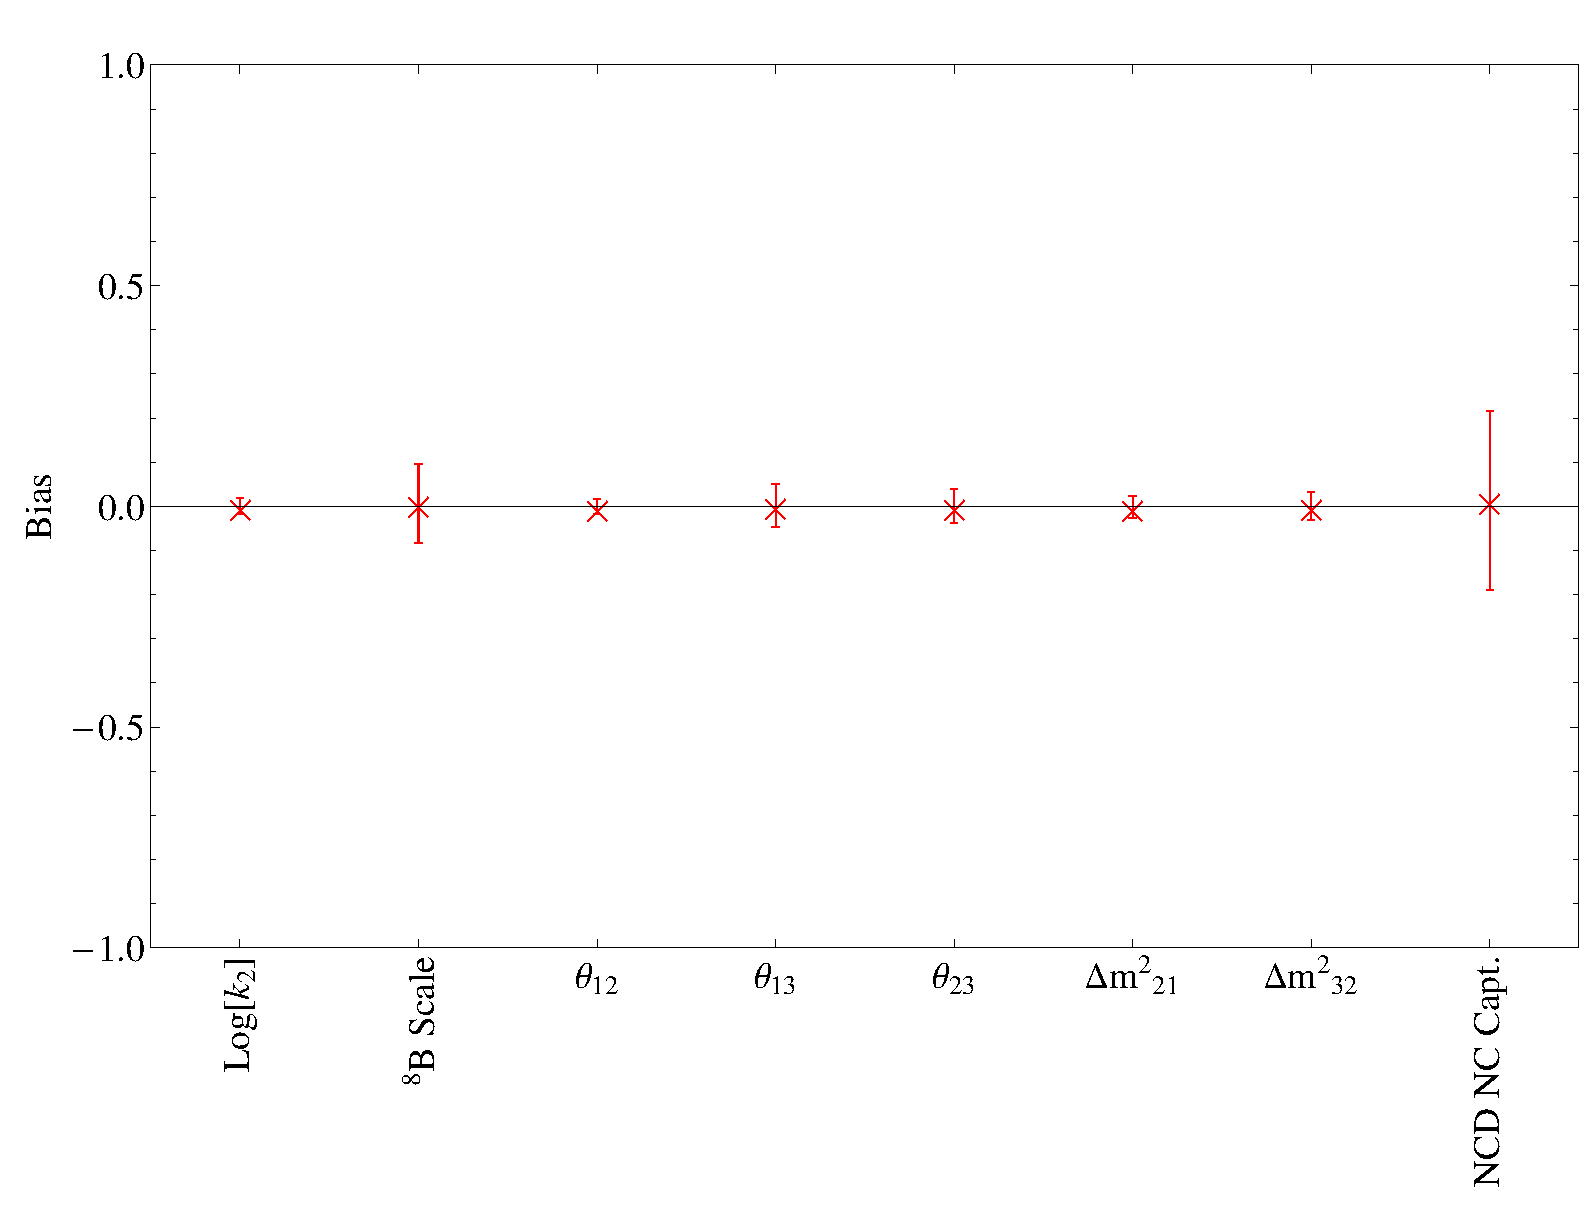
\includegraphics[width=0.82\columnwidth]{bias_nofit}
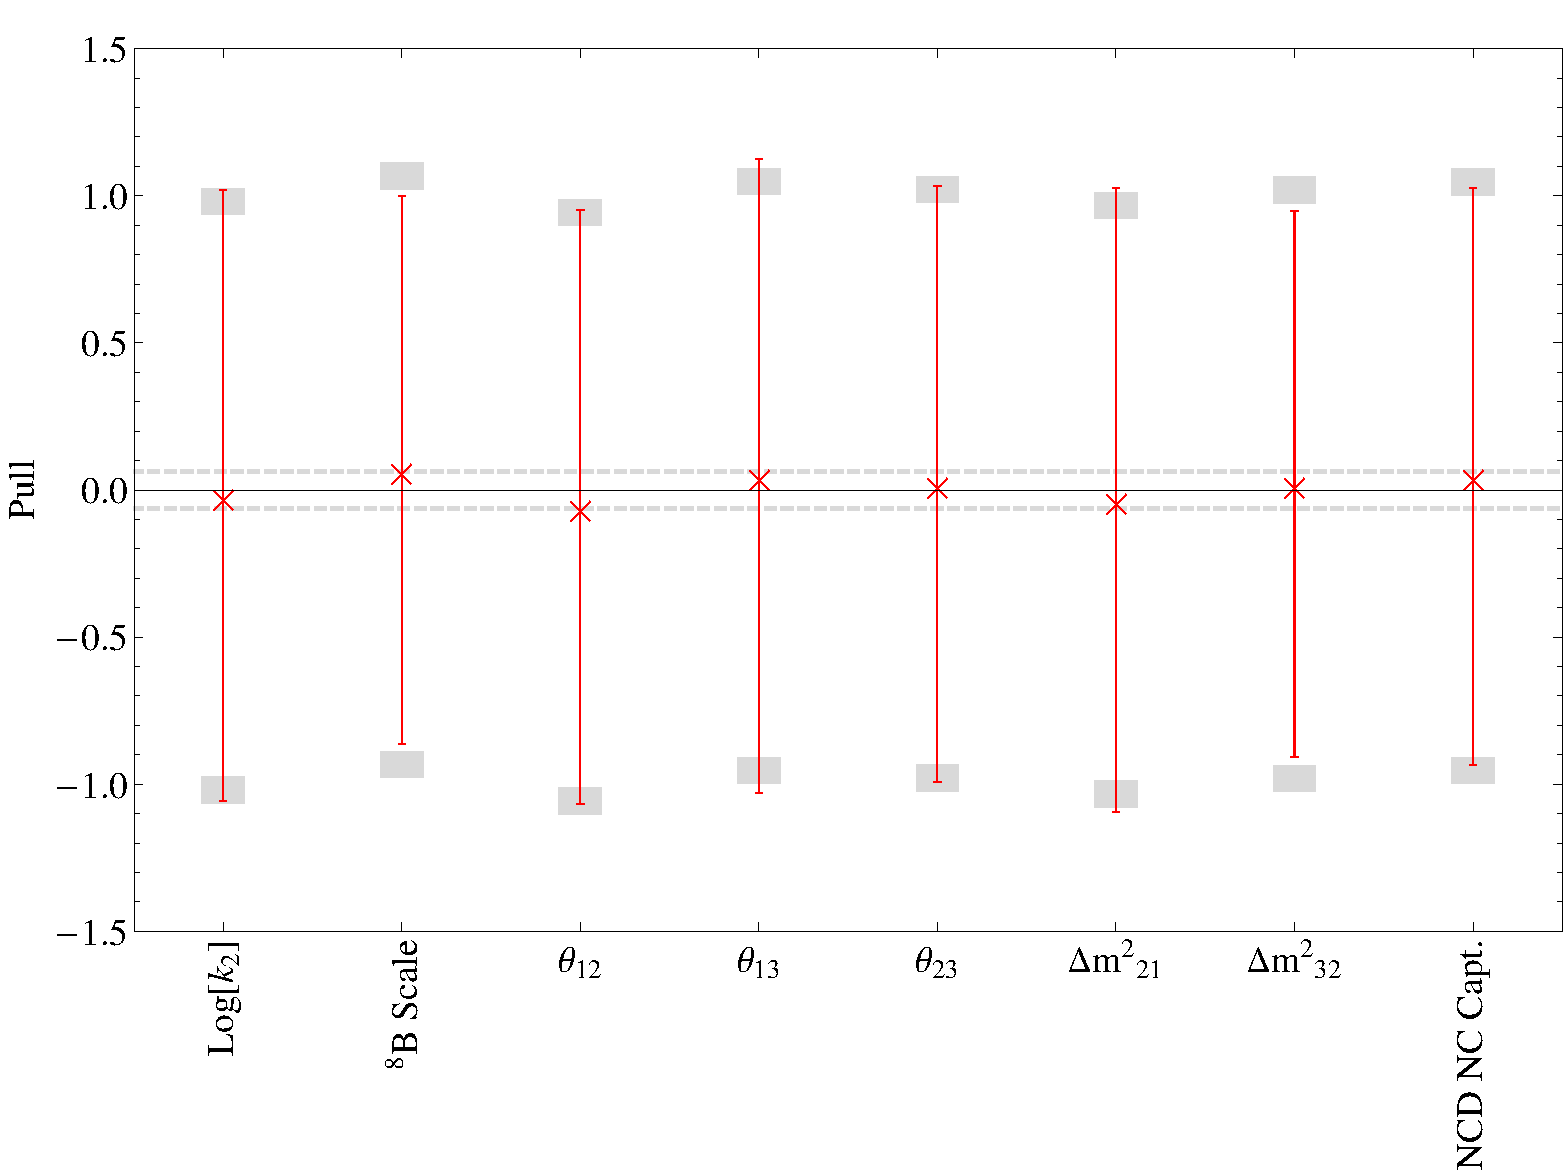
\includegraphics[width=0.82\columnwidth]{pull_nofit}
\caption{
The bias and pull of all fitted parameters with signal only datasets. Gray bars and dashed lines represent expected fluctuations due to limited statistics.
}
\label{fig:sigonly_biaspull}
\end{figure}

\begin{figure}
\centering
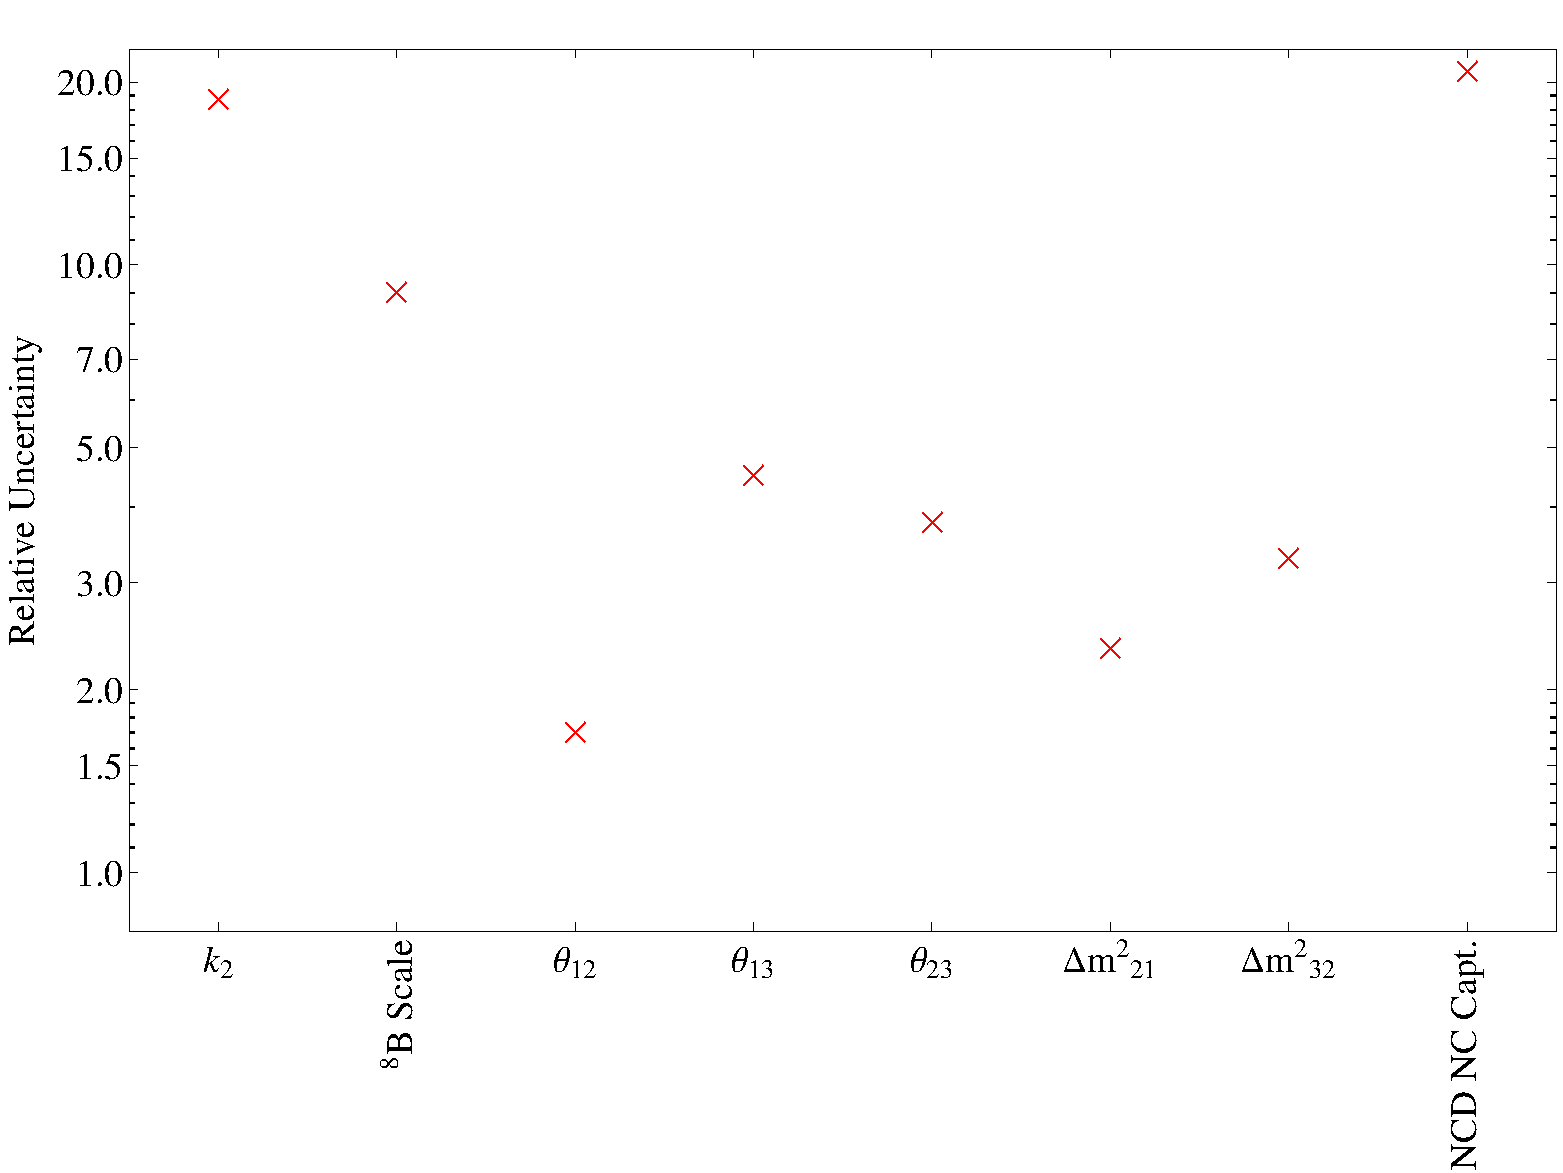
\includegraphics[width=0.85\columnwidth]{reluncert_nofit}
\caption{
The relative uncertainty of all fitted parameters with signal only datasets.
}
\label{fig:sigonly_reluncert}
\end{figure}

\clearpage

\subsection{Solar-Signal + High Statistics Backgrounds}

\begin{table}
\centering
\begin{tabular}{ccc}
\hline
Phase I Backgrounds & Phase II Backgrounds & Phase III Backgrounds \\ \hline \hline
AV neutrons & AV neutrons & External neutrons \\
Bi D$_2$O & Bi Salt & D$_2$O p.d. \\ 
Tl D$_2$O & Tl Salt & Atmospherics \\
hep CC & hep CC & hep CC \\
hep ES & hep ES & hep ES \\
hep NC & hep NC & hep NC \\
PMT $\beta$-$\gamma$ & PMT $\beta$-$\gamma$ \\ \hline
\end{tabular}
\caption{
These are the background event classes that are included in the high statistics background tests. This includes internal backgrounds, AV neutrons, PMT backgrounds, and other backgrounds with very high MC statistics.
}
\label{tbl:noextbitl_event_classes}
\end{table}

A subset of the fake 3-phase solar-signal only datasets from above were taken and combined with uncorrelated datasets of background events with high statistics.
The event classes shown in \Cref{tbl:noextbitl_event_classes} were added in this section. 
Due to the relatively lower statistics for background event classes, only 50 datasets could be created for each of the three $k_2$ values.
With QSigEx configured to only fit these event classes, the lifetime fit was performed on each dataset as described in \Cref{strategy}. 
The figures of merit for these tests are shown in \Cref{fig:noextbitl_bias,fig:noextbitl_pull,fig:noextbitl_reluncert}. 
Again, the results are consistent with an unbiased fit that properly estimates the fit uncertainties.

\begin{figure}
\centering
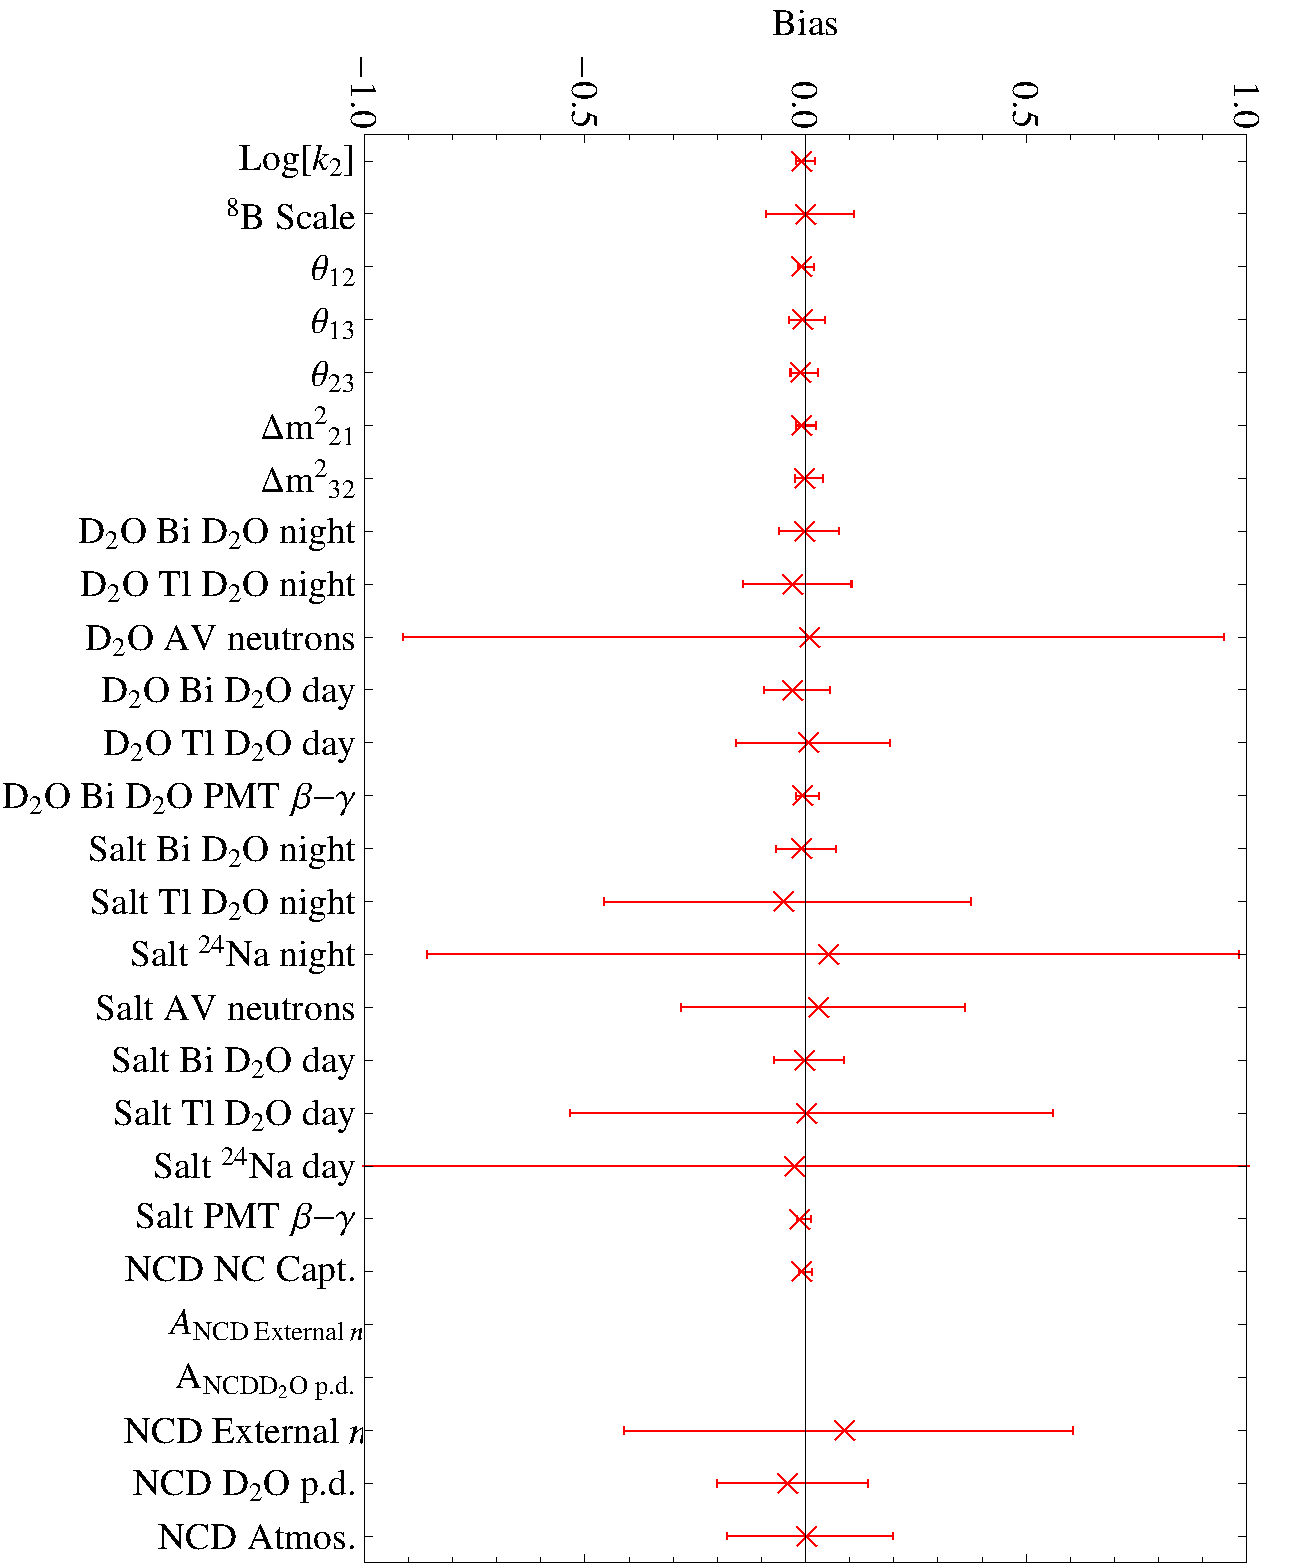
\includegraphics[width=0.85\columnwidth]{noextbitl_bias_nofit}
\caption{
The bias of all fitted parameters with signal + high stats backgrounds datasets.
}
\label{fig:noextbitl_bias}
\end{figure}

\begin{figure}
\centering
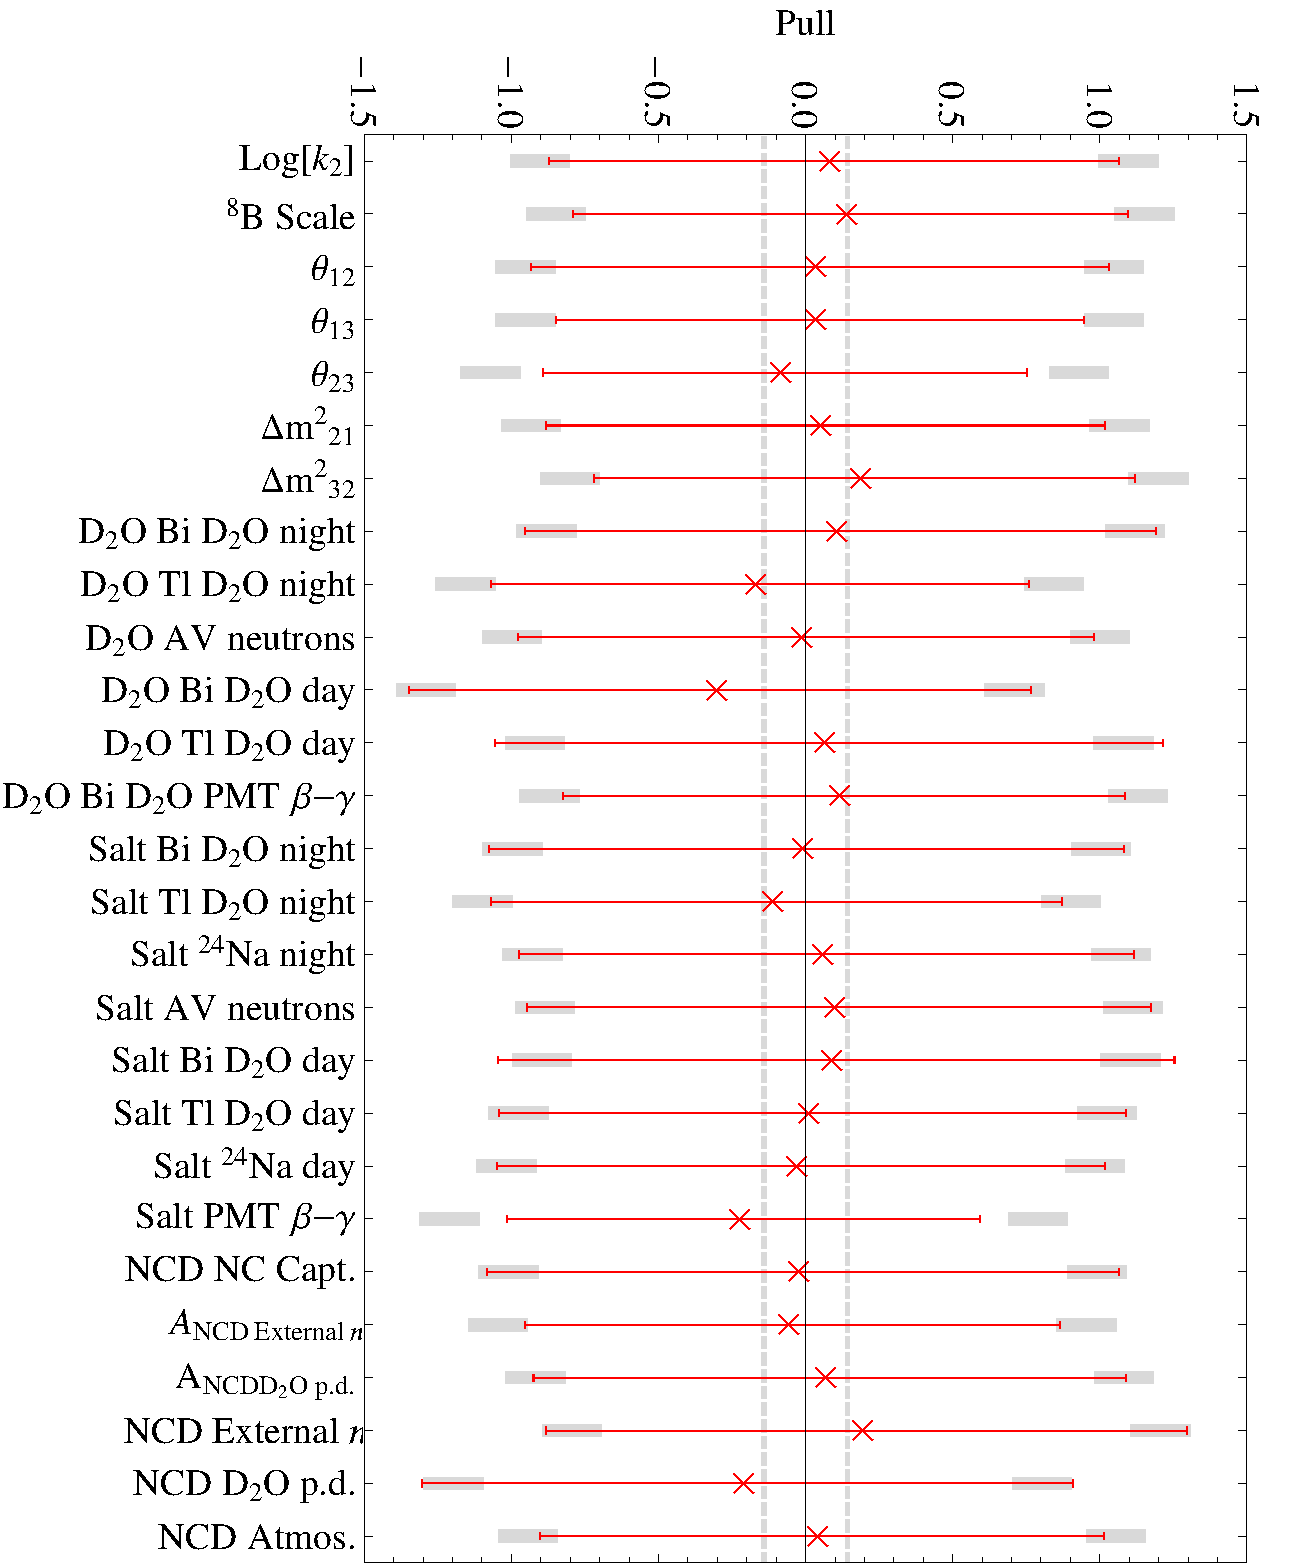
\includegraphics[width=0.85\columnwidth]{noextbitl_pull_nofit}
\caption{
The pull of all fitted parameters with signal + high stats backgrounds datasets. Gray bars and dashed lines represent expected fluctuations due to limited statistics.
}
\label{fig:noextbitl_pull}
\end{figure}

\begin{figure}
\centering
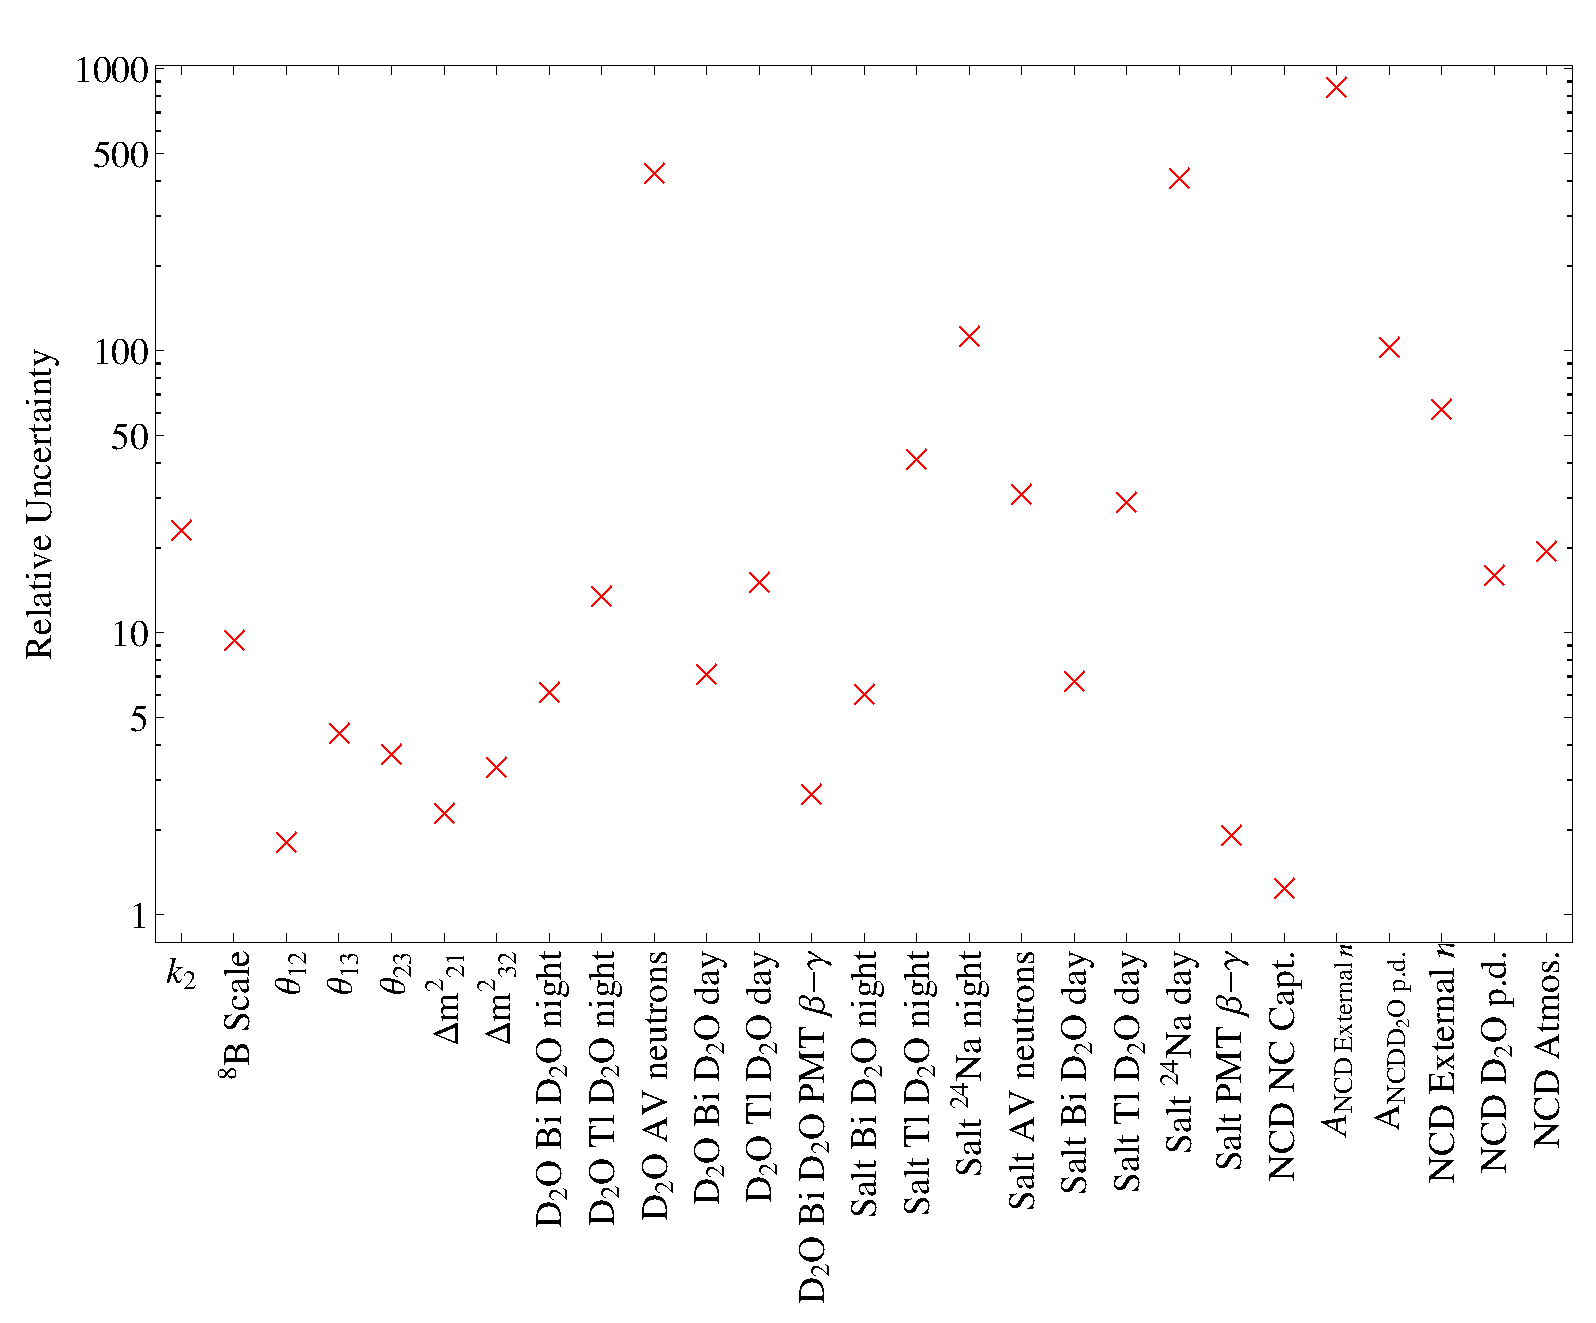
\includegraphics[width=0.85\columnwidth]{noextbitl_reluncert_nofit}
\caption{
The relative uncertainty of all fitted parameters with signal + high stats backgrounds datasets.
}
\label{fig:noextbitl_reluncert}
\end{figure}

\clearpage

\subsection{Solar-Signal + All Backgrounds}
\label{3phase_allbg}

\begin{table}
\centering
\begin{tabular}{ccc}
\hline
Phase I Backgrounds & Phase II Backgrounds & Phase III Backgrounds\\ \hline \hline
Bi AV bulk & Bi AV bulk & Strings p.d. \\
Tl AV bulk & Tl AV bulk & K2 p.d. \\
Bi H$_2$O & Bi H$_2$O & K5 p.d. \\
Tl H$_2$O & Tl H$_2$O & \\ \hline
\end{tabular}
\caption{
These are the background event classes that are added for the fits that include all backgrounds. This includes AV and external backgrounds for Phases I and II and photodisintegration for Phase III.
}
\label{tbl:allbg_event_classes}
\end{table}

A subset of the fake 3-phase high statistics background datasets from above were taken and combined with uncorrelated datasets of background events classes with low statistics.
The event classes shown in \Cref{tbl:allbg_event_classes} were added in this section and the datasets now include all relevant event classes.
Due to extremely limited statistics for some of these event classes, only 14 datasets for each of the three $k_2$ values could be created.
As was traditionally done for SNO analyses~\cite{plthesis}, these same events were resampled with a different random seed into 14 alternate datasets (c.f. the bootstrap method).
Comparing the results of these two datasets gives some information on statistical fluctuations due to limited statistics.
If the bias or pull looks particularly bad in one dataset but acceptable in the other, one can conclude that this effect is due to statistical fluctuations and not to errors in the fit procedure.
The figures of merit for these tests are shown in \Cref{fig:allbg_bias,fig:allbg_pull,fig:allbg_reluncert}. 
While fluctuations are larger, comparison between the two datasets looks more reasonable. 
Notably these results are comparable to ensemble testing of the published SNO 3-phase results \cite{3phase}.
One can therefore conclude that the fit is unbiased and properly predicting errors.

\begin{figure}
\centering
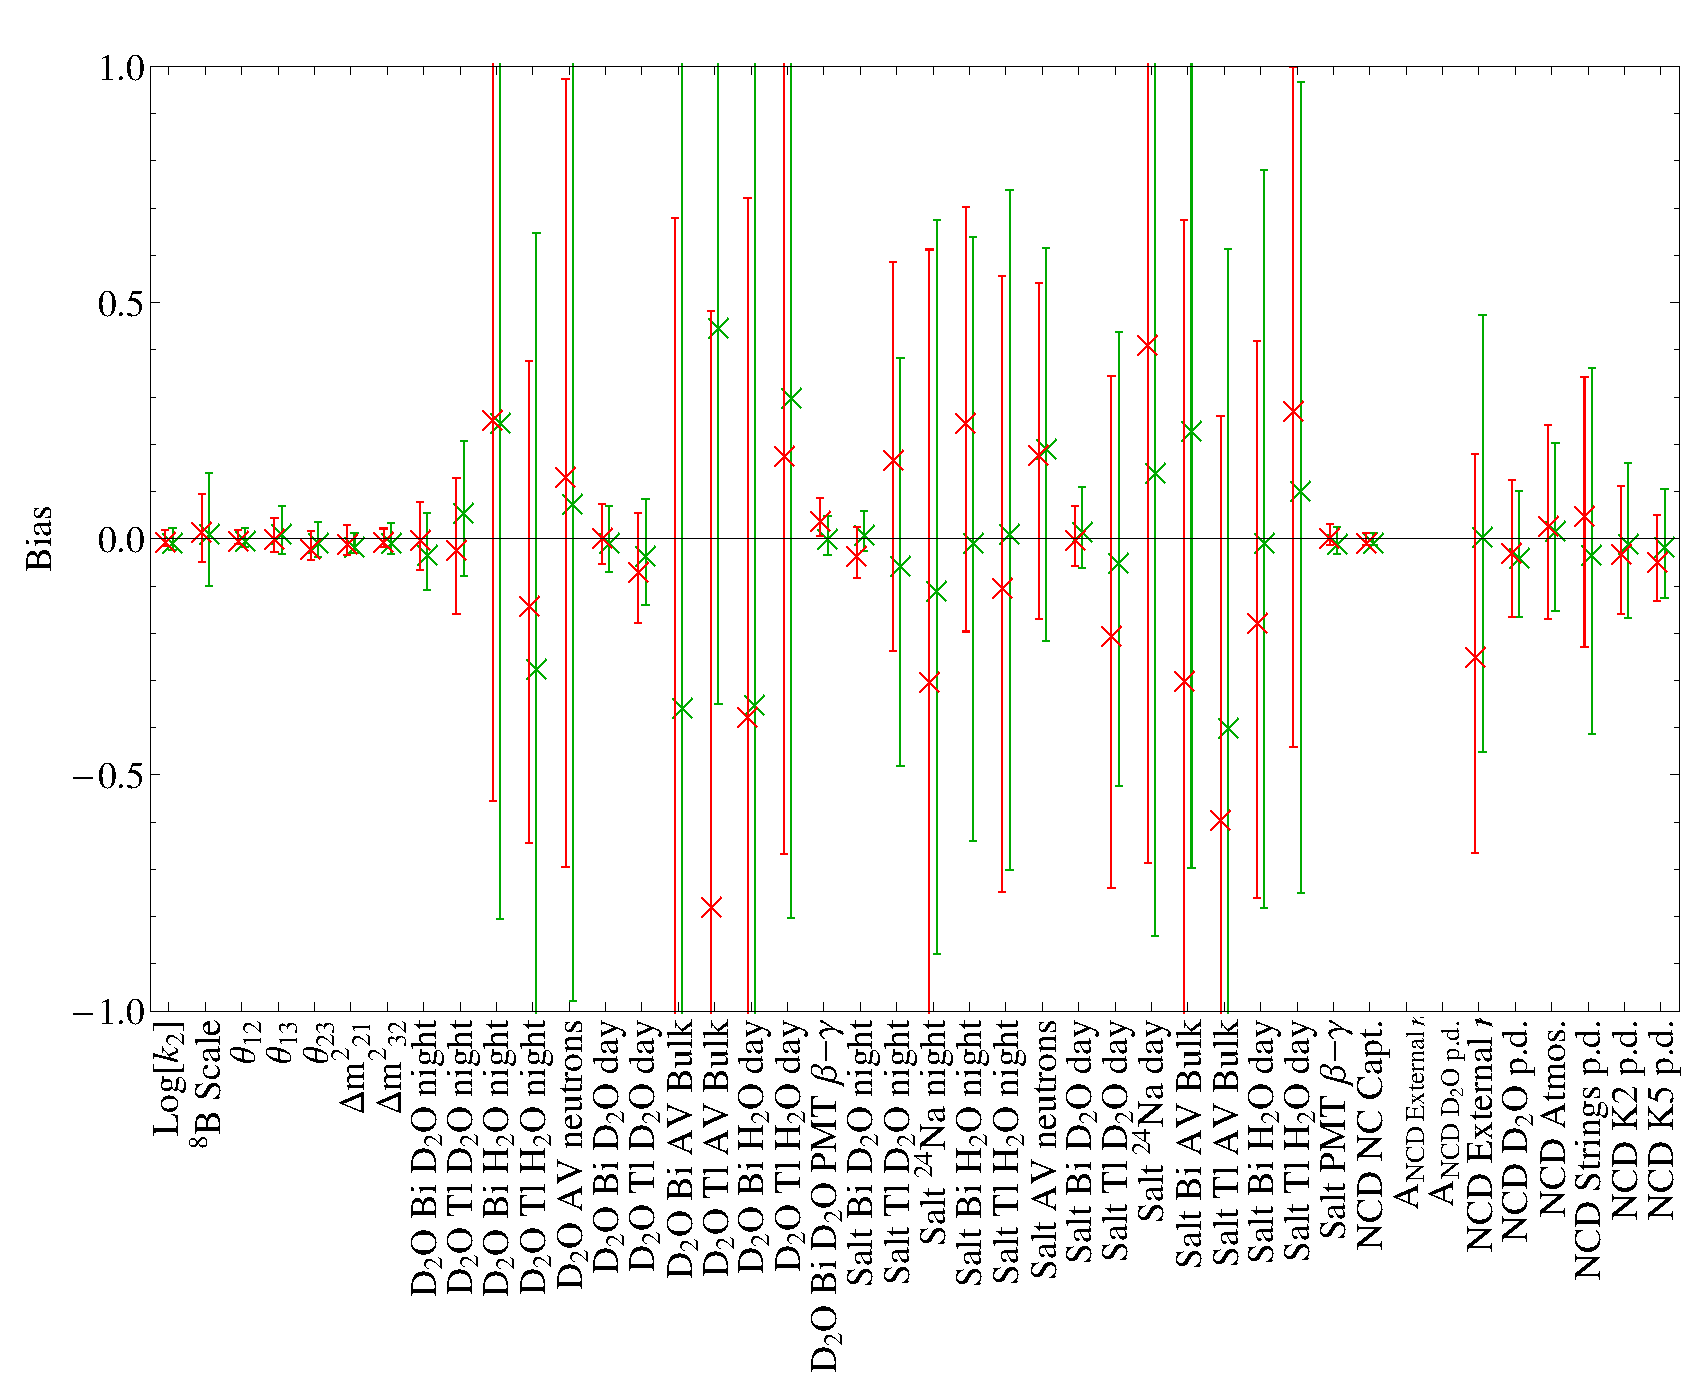
\includegraphics[width=0.85\columnwidth]{bias_combined}
\caption{
The bias of all fitted parameters with signal + all backgrounds datasets. The alternate ensemble results are shown in green for comparison.
}
\label{fig:allbg_bias}
\end{figure}

\begin{figure}
\centering
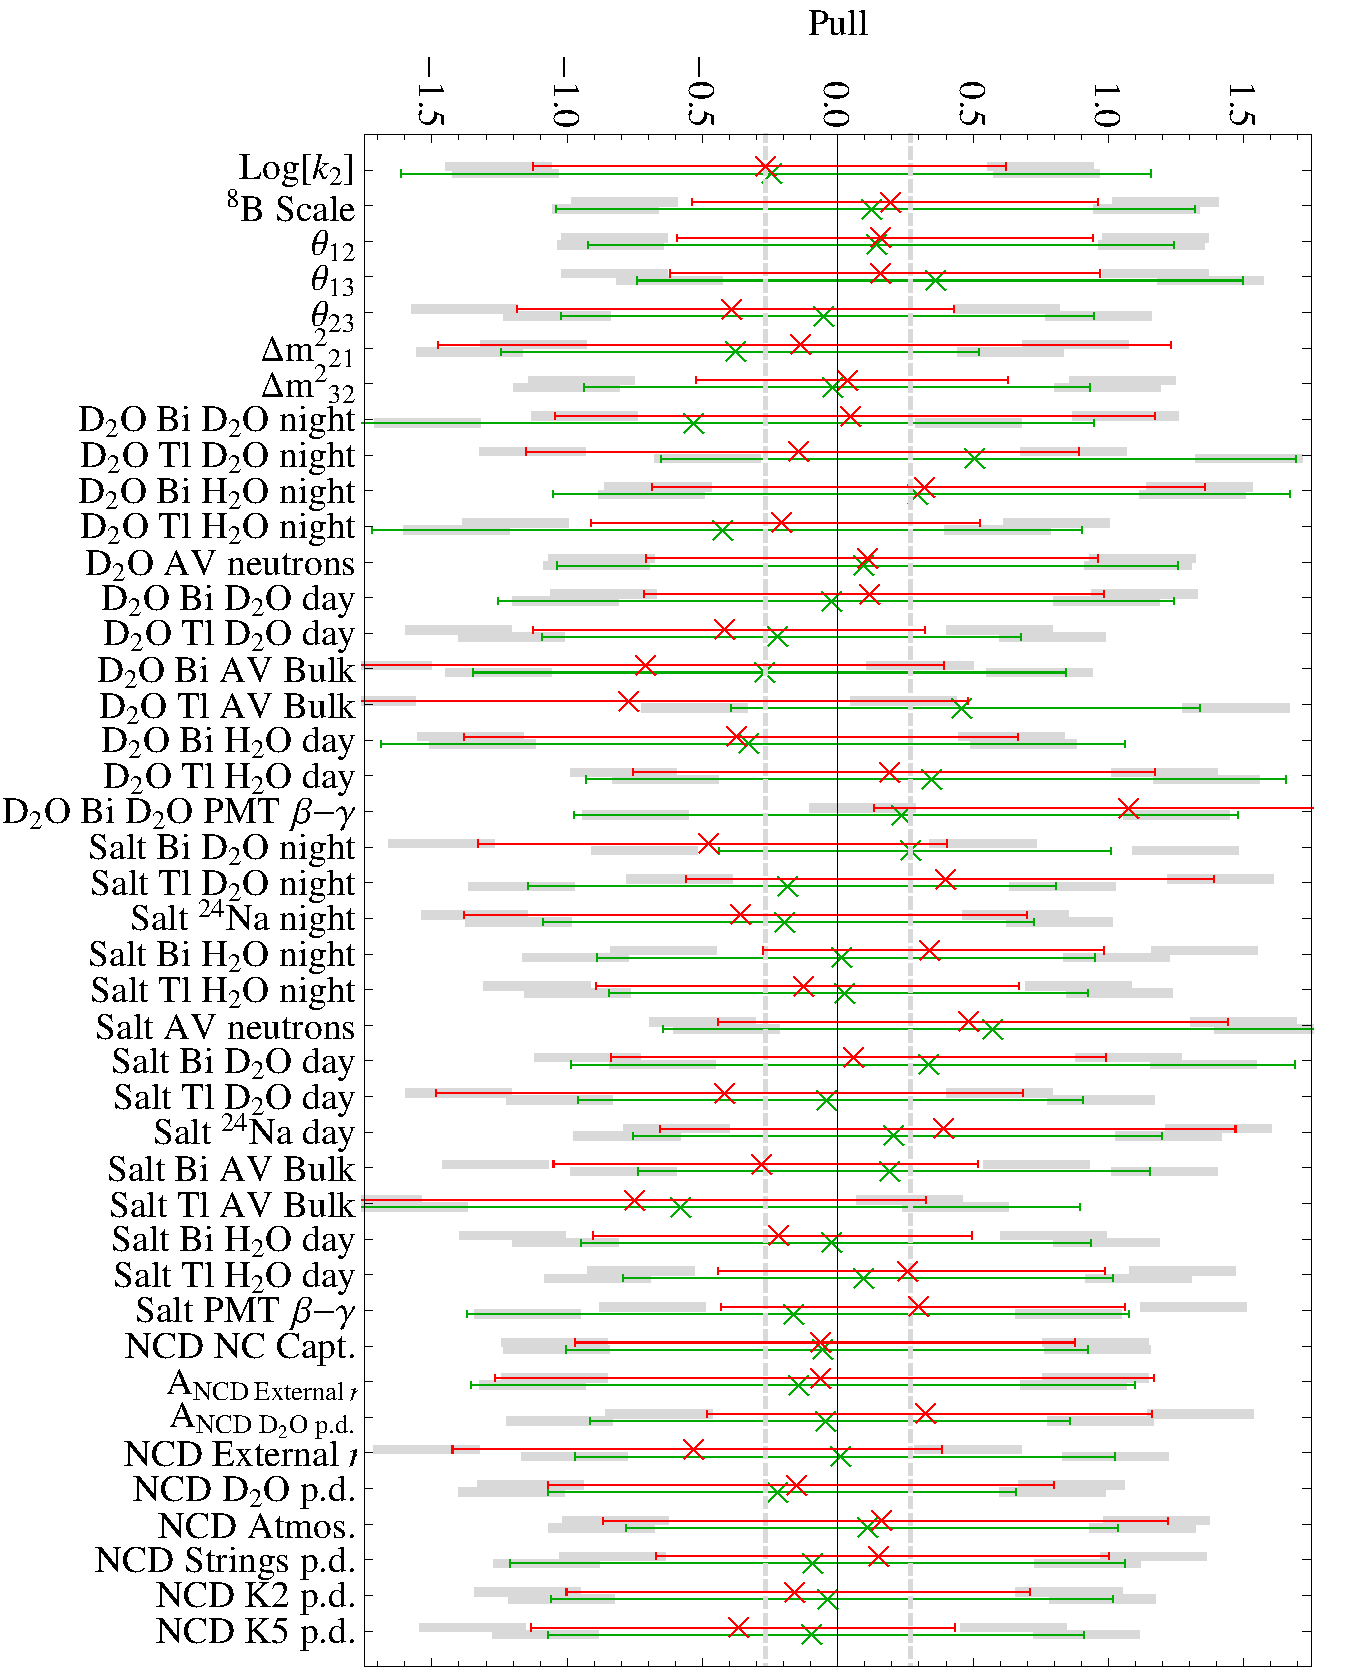
\includegraphics[width=0.85\columnwidth]{pull_combined}
\caption{
The pull of all fitted parameters with signal + all backgrounds datasets. Gray bars and dashed lines represent expected fluctuations due to limited statistics. The alternate ensemble results are shown in green for comparison.
}
\label{fig:allbg_pull}
\end{figure}

\begin{figure}
\centering
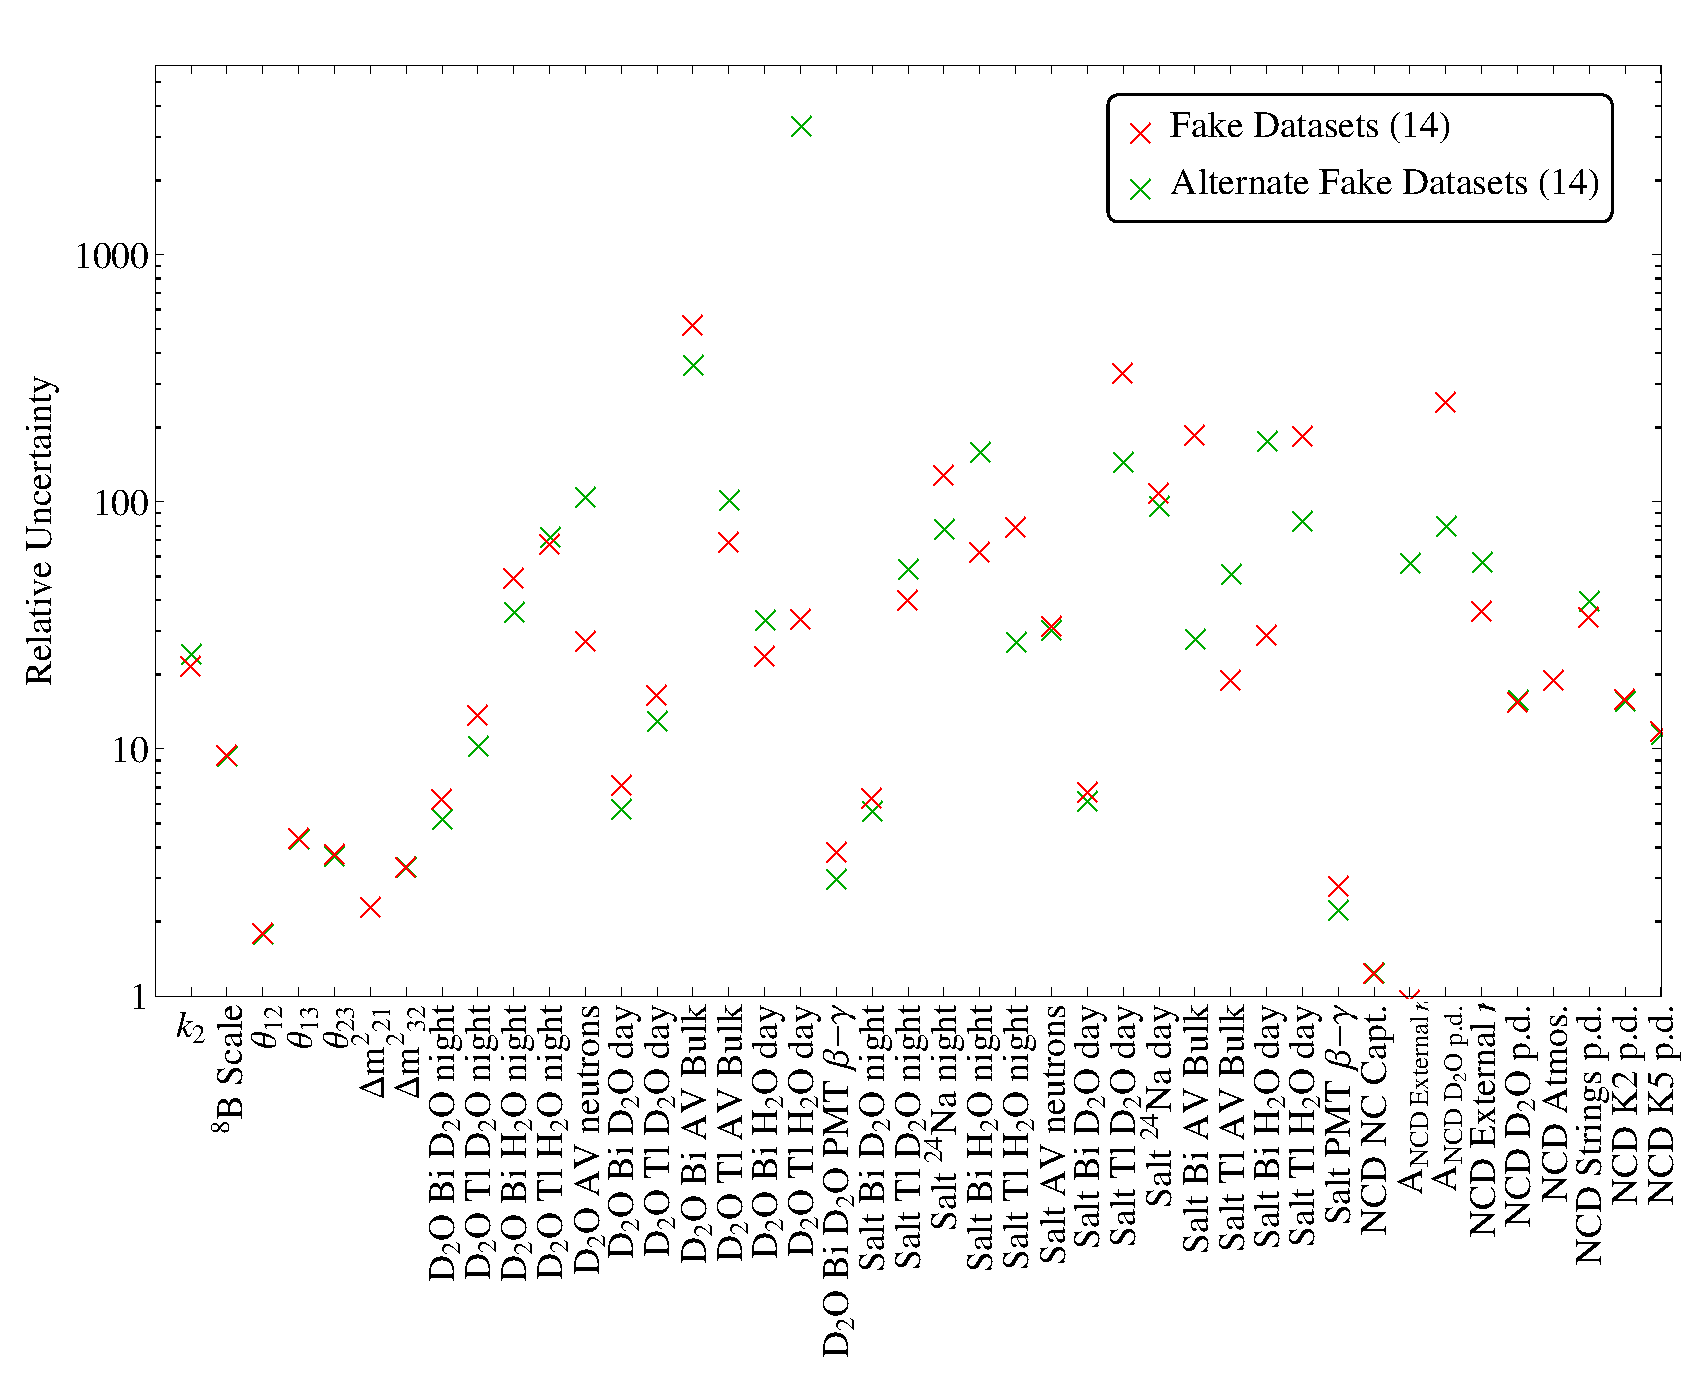
\includegraphics[width=0.85\columnwidth]{reluncert_combined}
\caption{
The relative uncertainty of all fitted parameters with signal + all backgrounds datasets. The alternate ensemble results are shown in green for comparison.
}
\label{fig:allbg_reluncert}
\end{figure}

\clearpage

\subsection{Independent Impact of Systematics}

The following systematic tests were done at the best fit values for a fake dataset of comparable statistics to the SNO 3-phase dataset with all backgrounds included. 
This fake dataset was seeded with $k_2 = 10^{-4}$~s/eV and had the $^8$B flux seeded and fixed at the SSM central value.
The parameters considered here include all parameters whose uncertainties are propagated with the shift-and-refit method. 
\Cref{fig:detector_systematics1,fig:detector_systematics2} show the individual contributions of these parameters independently.
In the final fit these systematics will be propagated by simultaneously shifting all parameters and refitting as described in \Cref{systematics}, however, for this test it was desired to know the impact of each parameter.
When summed in quadrature, the total uncertainty on $k_2$ is found to be $^{+13.4\%}_{-9.03\%}$.

\begin{figure}
\centering
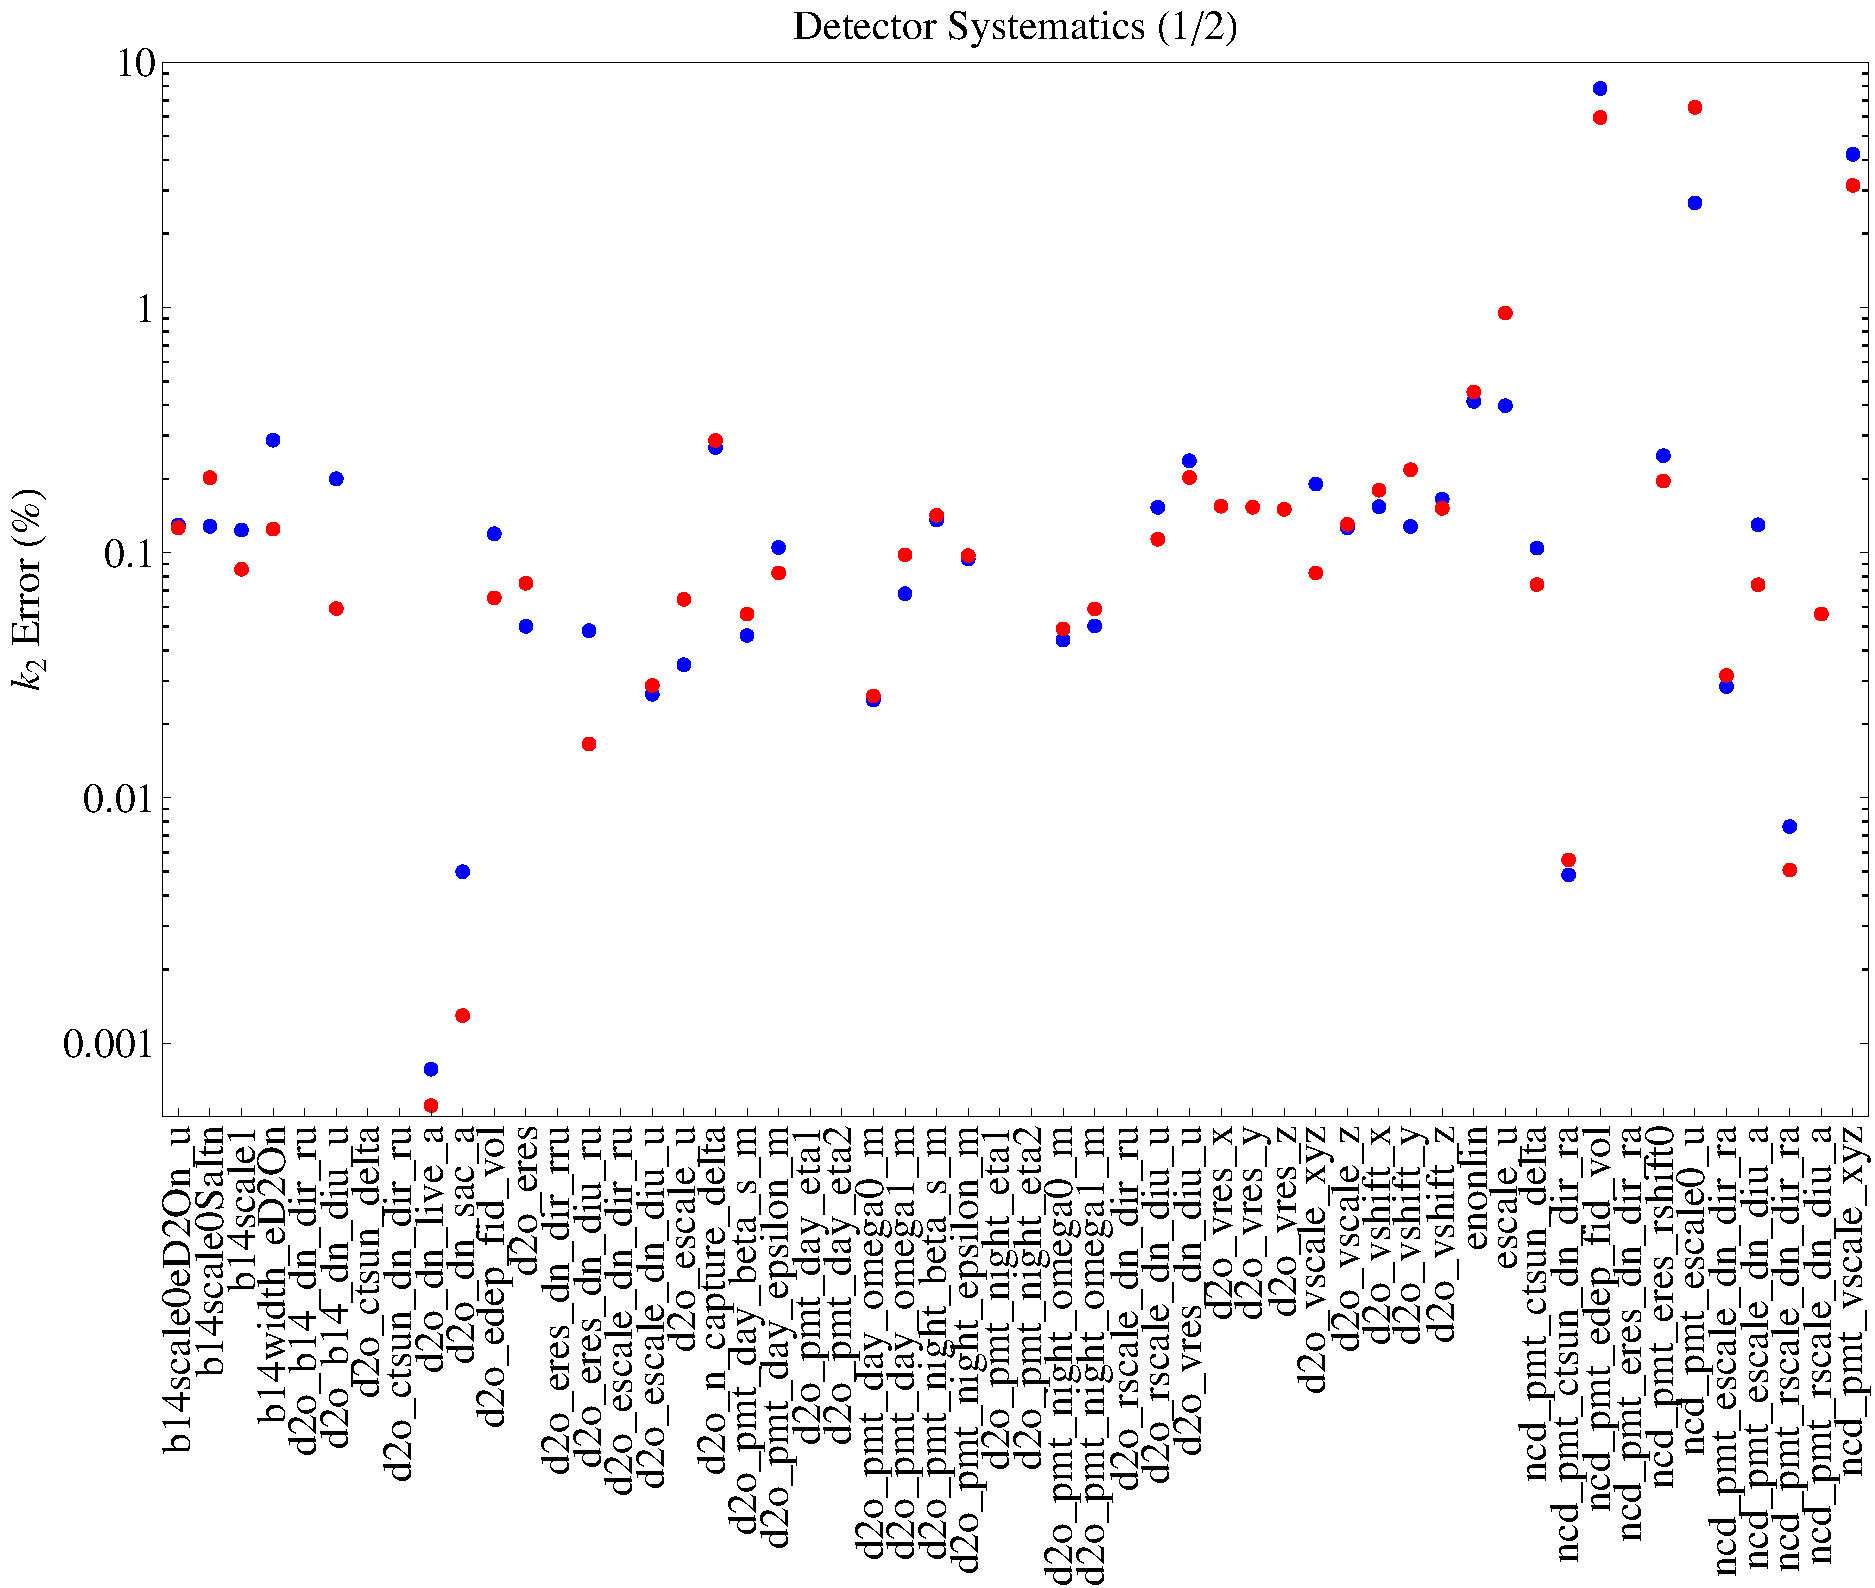
\includegraphics[width=0.85\columnwidth]{basic_1_2}
\caption{The calculated systematic effect on $k_2$ from the first half of the detector systematic parameters in the fit is shown here. Red represents positive (blue, negative) fractional error.}
\label{fig:detector_systematics1}
\end{figure}

\begin{figure}
\centering
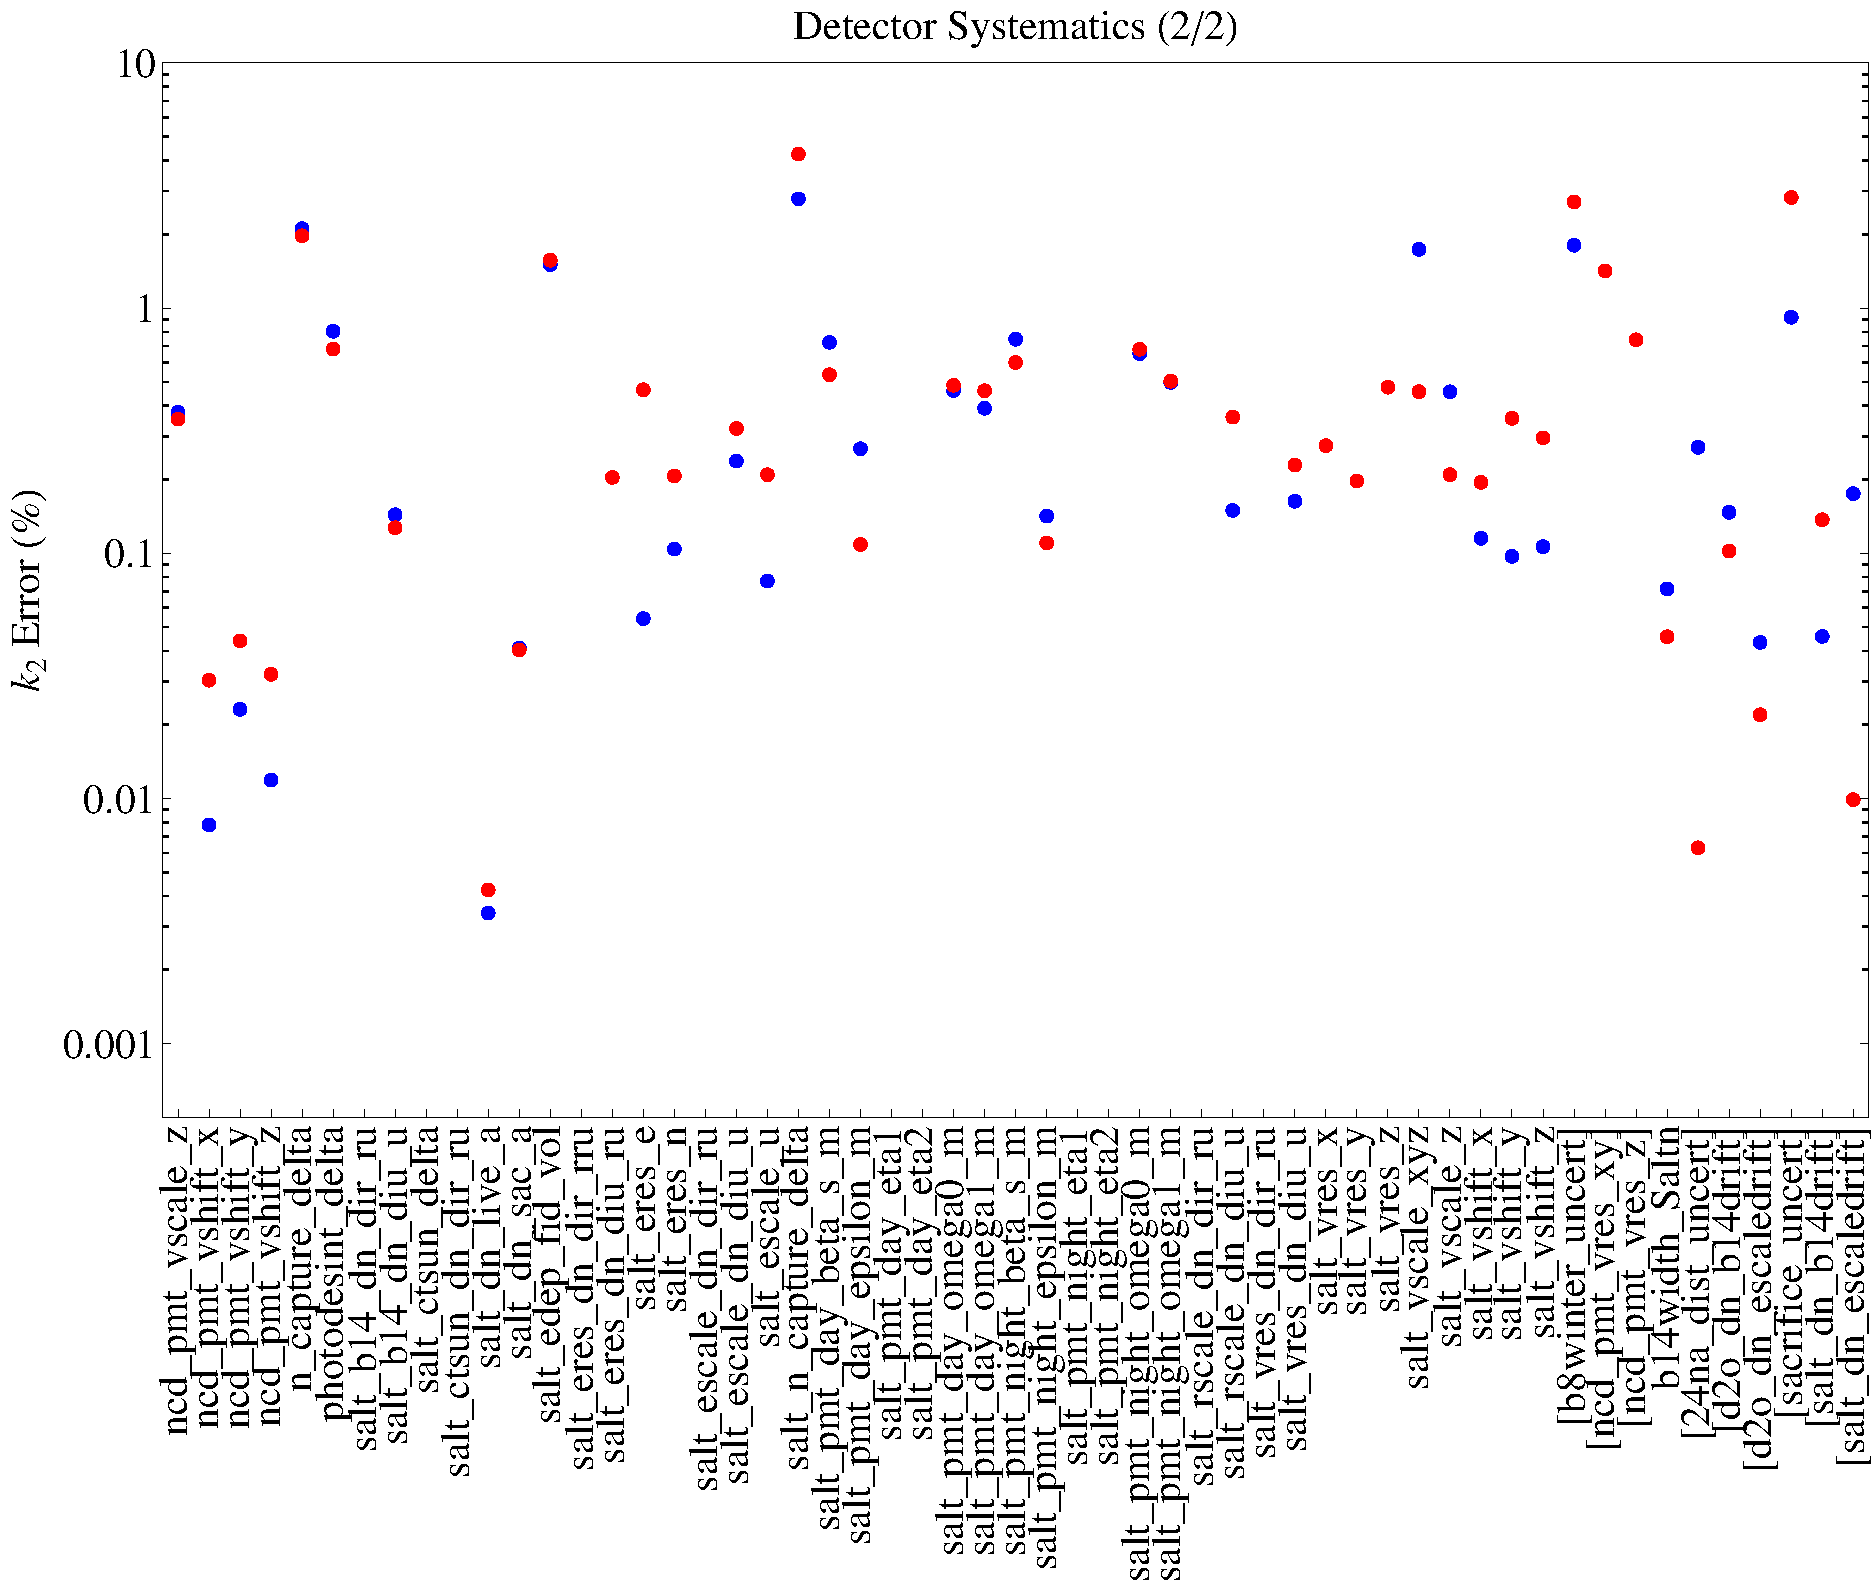
\includegraphics[width=0.85\columnwidth]{basic_2_2}
\caption{The calculated systematic effect on $k_2$ from the second half of the detector systematic parameters in the fit is shown here. Red represents positive (blue, negative) fractional error.}
\label{fig:detector_systematics2}
\end{figure}


\clearpage 

\section{\nicefrac{1}{3} Dataset}
\label{third}

Using 1/3 of the SNO dataset --- the same 1/3 dataset used in testing the historical 3-phase fits --- the fit was run as described in \Cref{strategy}. 
To reduce computational power required for this test, the central values of scanned nuisance parameters from the 3-phase Pee+Pea fit \cite{3phase} were used. 
These are nominally uncorrelated with neutrino parameters, and would take a very long time to iteratively scan with little gain.
This scan will, of course, be done for the full dataset.
The scan of $k_2$ and the $^8$B flux are shown in \Cref{fig:third_scans}.
The neutrino parameters are shown relative to their priors in \Cref{fig:priors_third}.
The observable projections for the minimum and with $k_2$ fixed to infinity are shown in \Cref{third_observables}.

There is a 1-sigma minimum for $k_2$ at a central value of of $4.62\times10^{-4}$~s/eV.
This minimum is almost consistent with infinite lifetime at the one sigma level, and has a one sigma lower bound of $2.40\times10^{-4}$~s/eV.
The fitted value of the $^8$B flux is $5.77^{+0.58}_{-0.58}\times10^6$~cm$^{-2}$s$^{-1}$ ($1.01\pm0.10 \times \Phi_{8B_{BS05(OP)}}$), which is quite consistent with the SSM predictions.
With $k_2$ fixed at infinity the $^8$B flux fits to $5.19^{+0.16}_{-0.16}\times10^6$~cm$^{-2}$s$^{-1}$ ($0.91\pm0.03 \times \Phi_{8B_{BS05(OP)}}$).
Both flux measurements are consistent with previous 3-phase SNO results: $5.23^{+0.16}_{-0.16}\times10^6$~cm$^{-2}$s$^{-1}$ ($0.92\pm0.03 \times \Phi_{8B_{BS05(OP)}}$).

\begin{figure}
\centering
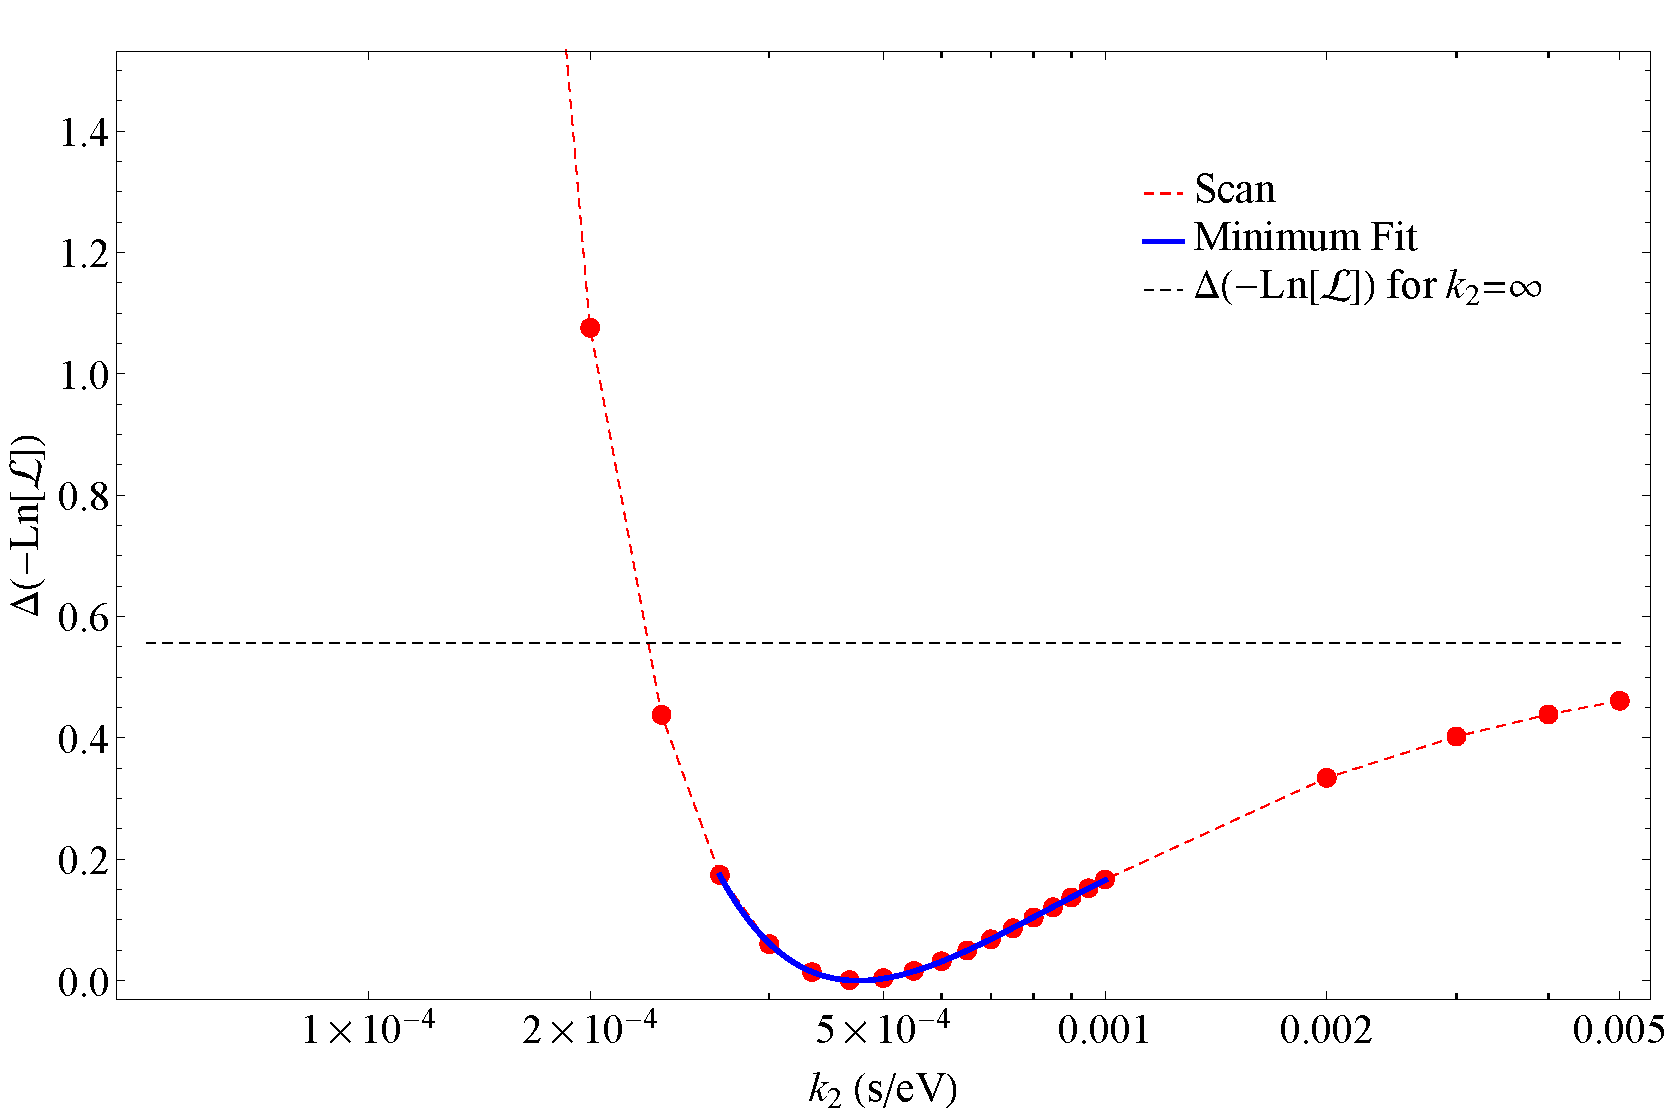
\includegraphics[width=0.85\columnwidth]{k2_scan_third} \\
\vspace{12pt}
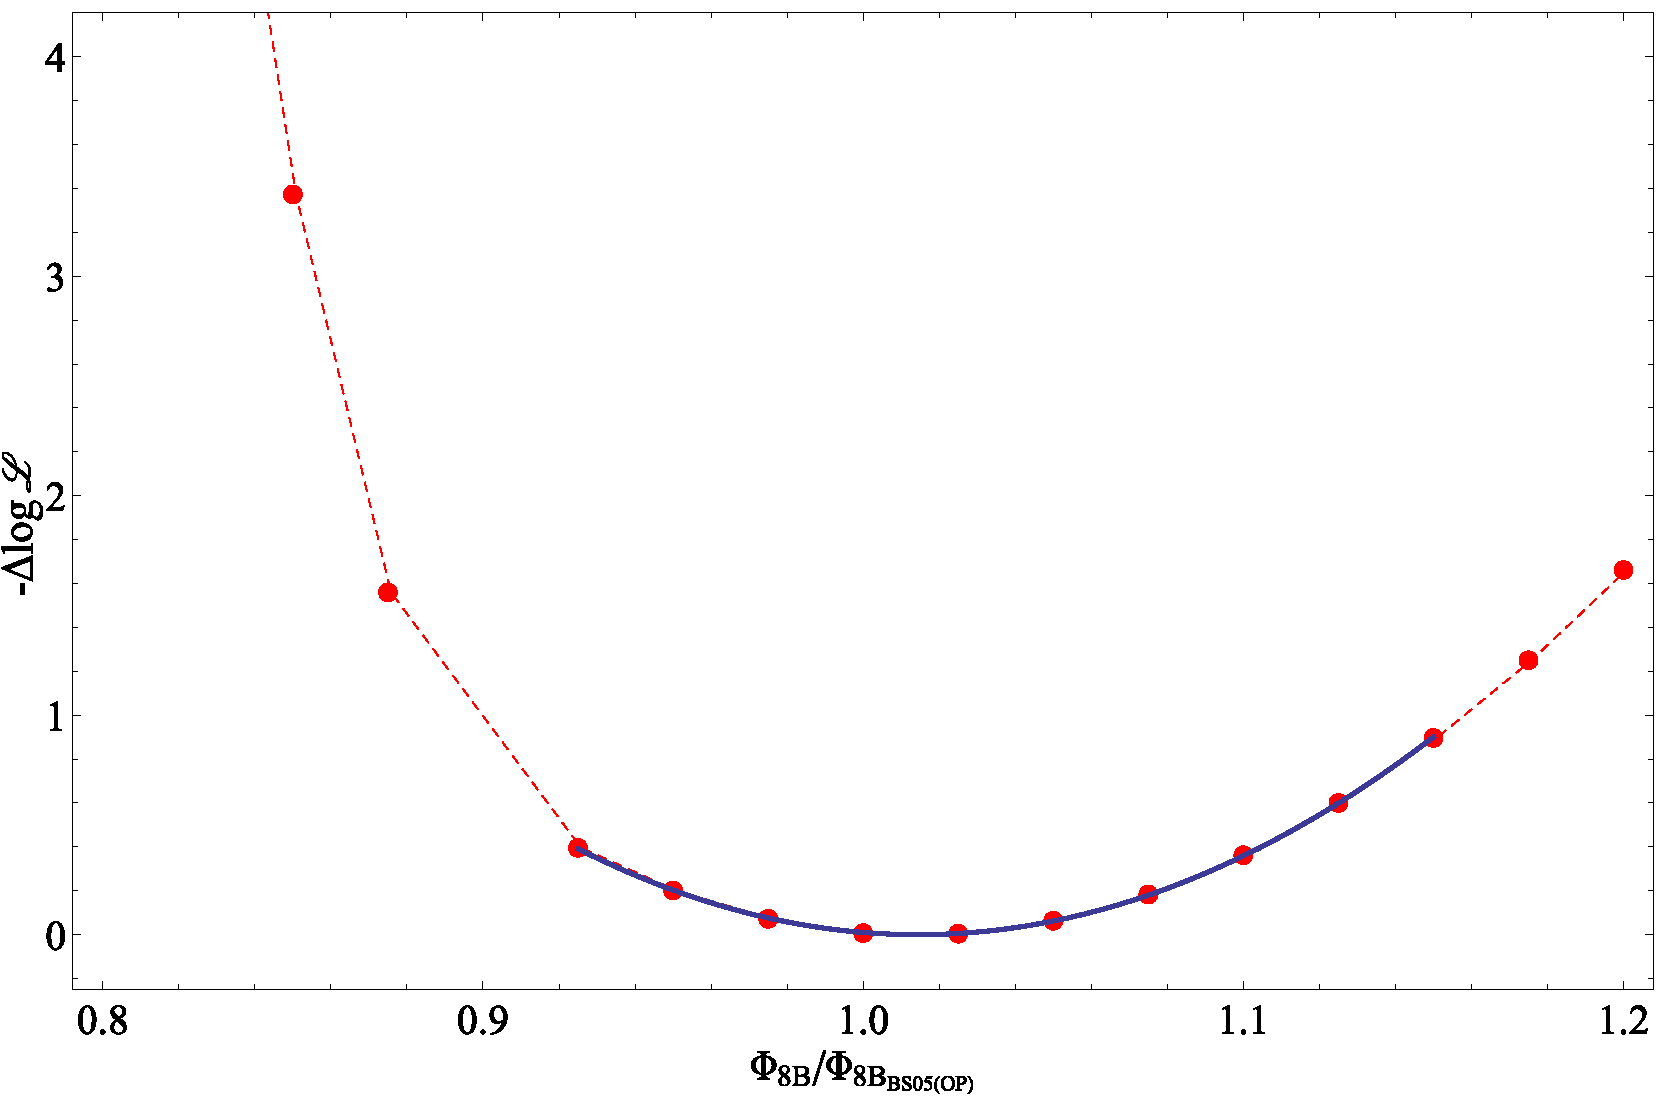
\includegraphics[width=0.85\columnwidth]{flux_scan_third}
\caption{The scans of $k_2$ and the $^8$B flux for the 1/3 dataset. The red points are the scan values, and the blue line is a fit to the minimum.}
\label{fig:third_scans}
\end{figure}

\begin{figure}
\centering
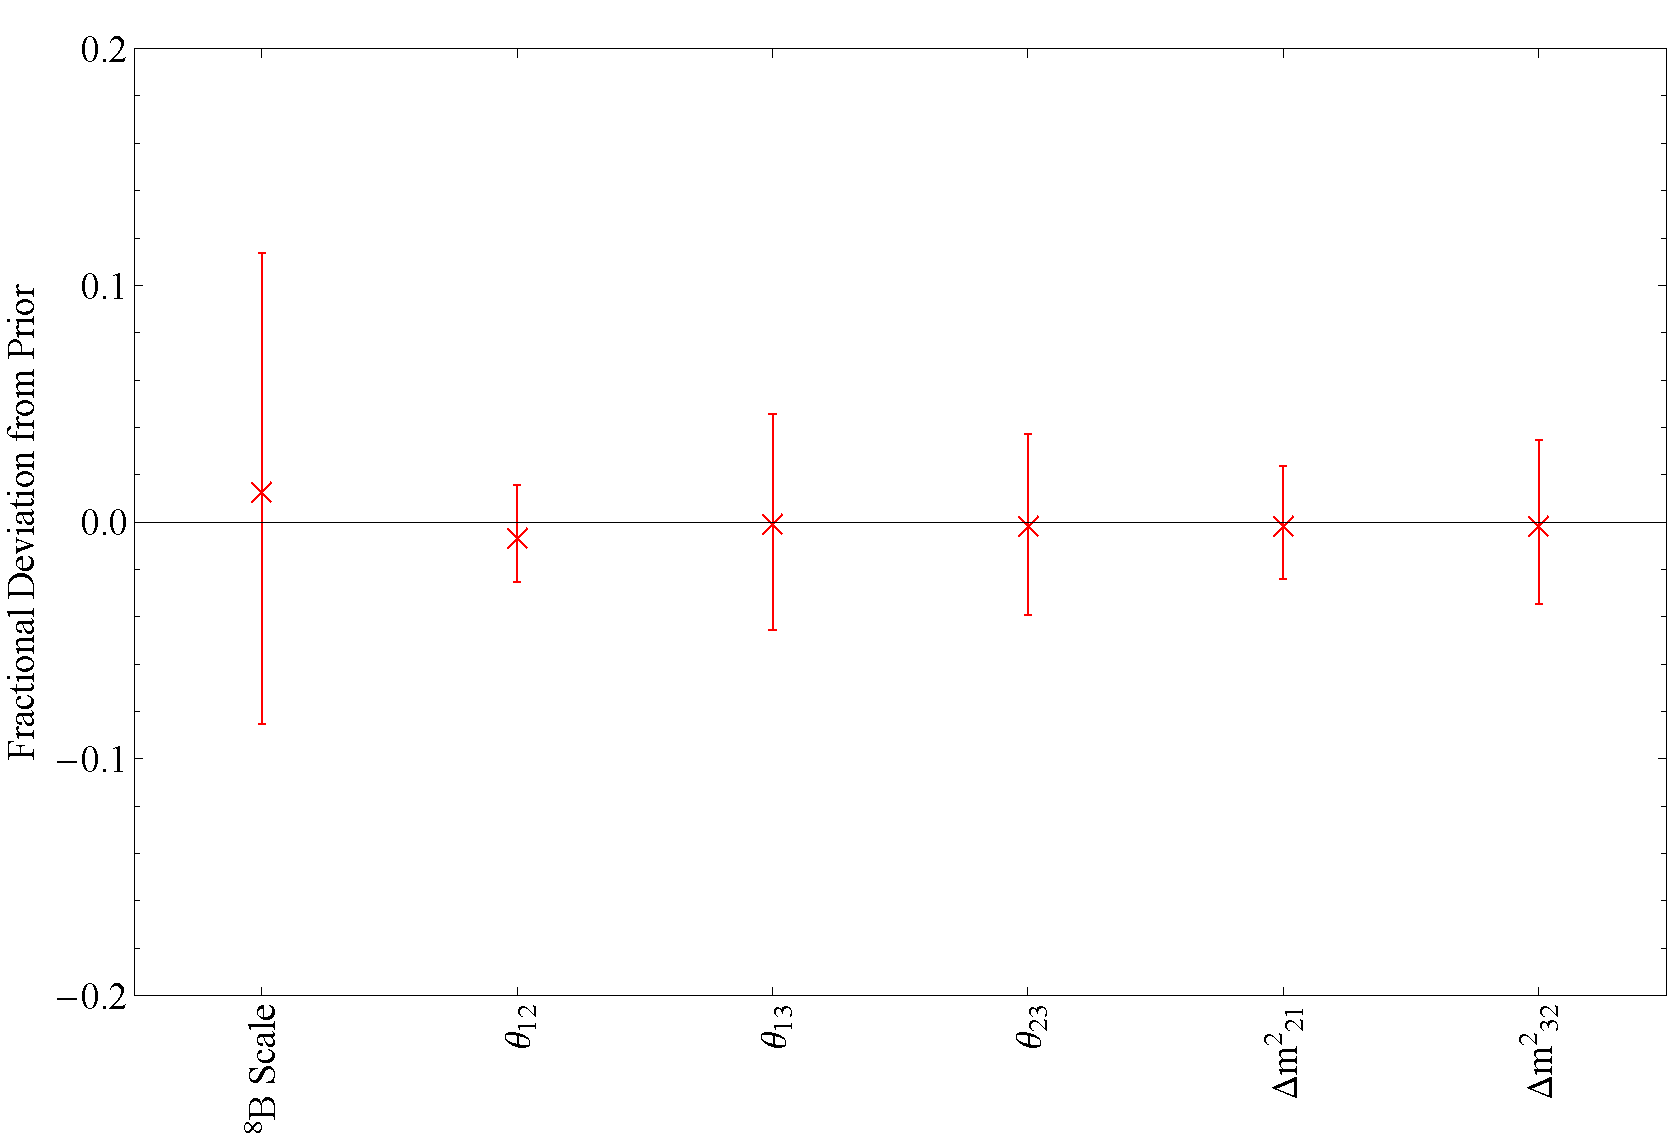
\includegraphics[width=0.85\columnwidth]{prior_deviation_third}
\caption{The fractional deviation of each neutrino parameter with a prior constraint from its prior. The errors shown are the fractional errors of the fit.}
\label{fig:priors_third}
\end{figure}

\clearpage

\section{Final Results}
\label{final}

Now with the entire SNO dataset, the fit was run as described in \Cref{strategy}. 
As a preliminary step, the systematics identified in the previous 3-phase analysis as requiring scanning were scanned iteratively until a global minimum was found.
Using the central values for the systemtics, both $k_2$ and $^8$B flux were then scanned with the systematic parameters fixed at their central values, and are shown in \Cref{fig:final_scans}.
The neutrino parameters are shown relative to their priors at the minimum of this scan in \Cref{fig:priors_final}.
The observable projections for the minimum and with $k_2$ fixed to infinity are shown in \Cref{final_observables}.
The likelihood profile including systematic uncertainties is compared to the likelihood profile without systematics in \Cref{fig:systematic_scans}.

The minimum for $k_2$ observed in the 1/3 data fit is still present in this fit (at higher significance) at a central value of of $3.45^{+5.50}_{-1.68}\times10^{-4}$~s/eV where the uncertainty given is the total uncertainty.
This minimum is consistent with infinite lifetime at a bit over $85\%$ confidence, and sets a $90\%$ confidence lower bound at $>8.08\times10^{-5}$~s/eV.
This lower bound was found by applying Wilks' theorem to the systematically broadened likelihood, i.e. when the $-2\Delta\log{L}$ from the minimum crosses $2.71$.
The fitted value of the $^8$B flux is $6.08^{+0.47}_{-0.47}$(stat.)$^{+0.21}_{-0.22}$(syst.)$\times10^6$~cm$^{-2}$s$^{-1}$ ($1.07\pm0.10 \times \Phi_{8B_{BS05(OP)}}$), which is quite consistent with the SSM predictions and constraint.
With $k_2$ fixed at infinity the $^8$B flux fits to $5.22^{+0.16}_{-0.16}\times10^6$~cm$^{-2}$s$^{-1}$ ($0.92\pm0.03 \times \Phi_{8B_{BS05(OP)}}$).
The flux measurement with $k_2$ fixed at infinity is expected to reproduce previous 3-phase results, and is quite consistent consistent with those results: $5.23^{+0.16}_{-0.16}\times10^6$~cm$^{-2}$s$^{-1}$ ($0.92\pm0.03 \times \Phi_{8B_{BS05(OP)}}$).
There is some tension between the SNO result and the flux fitted with with $k_2$ floating, however, they are consistent at two sigma. 

\begin{figure}
\centering
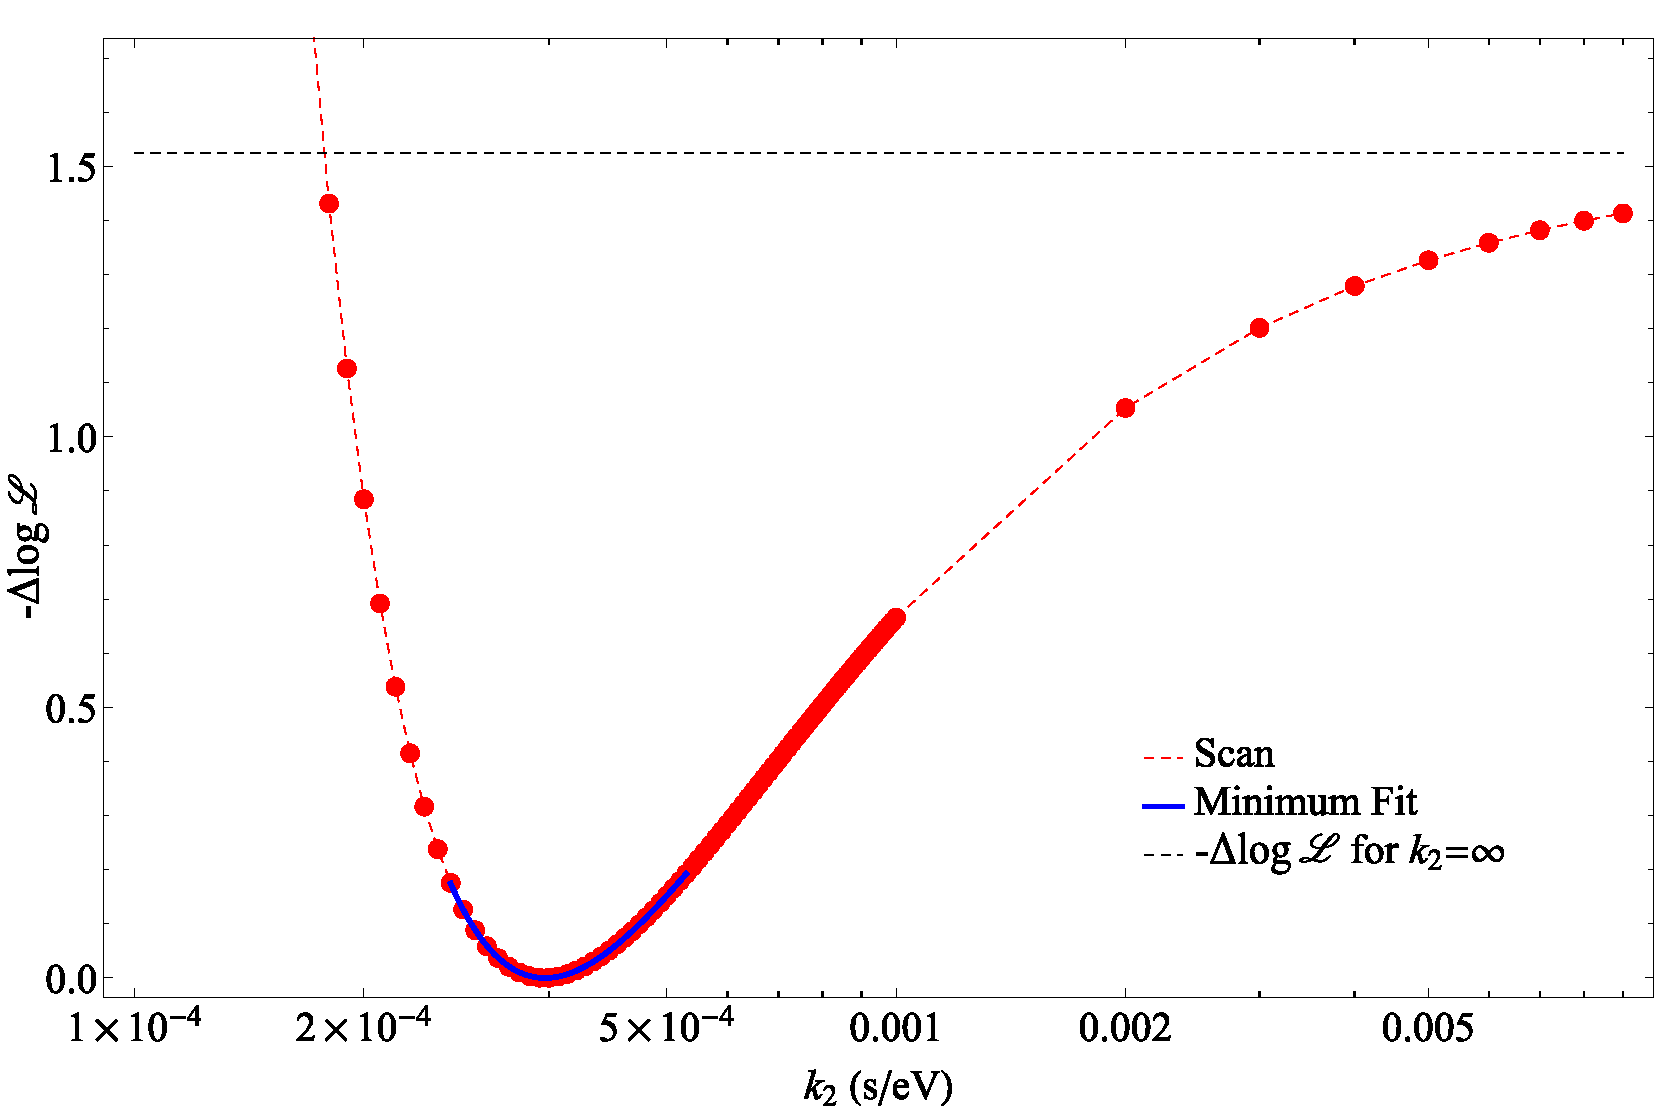
\includegraphics[width=0.85\columnwidth]{k2_scan_final} \\
\vspace{12pt}
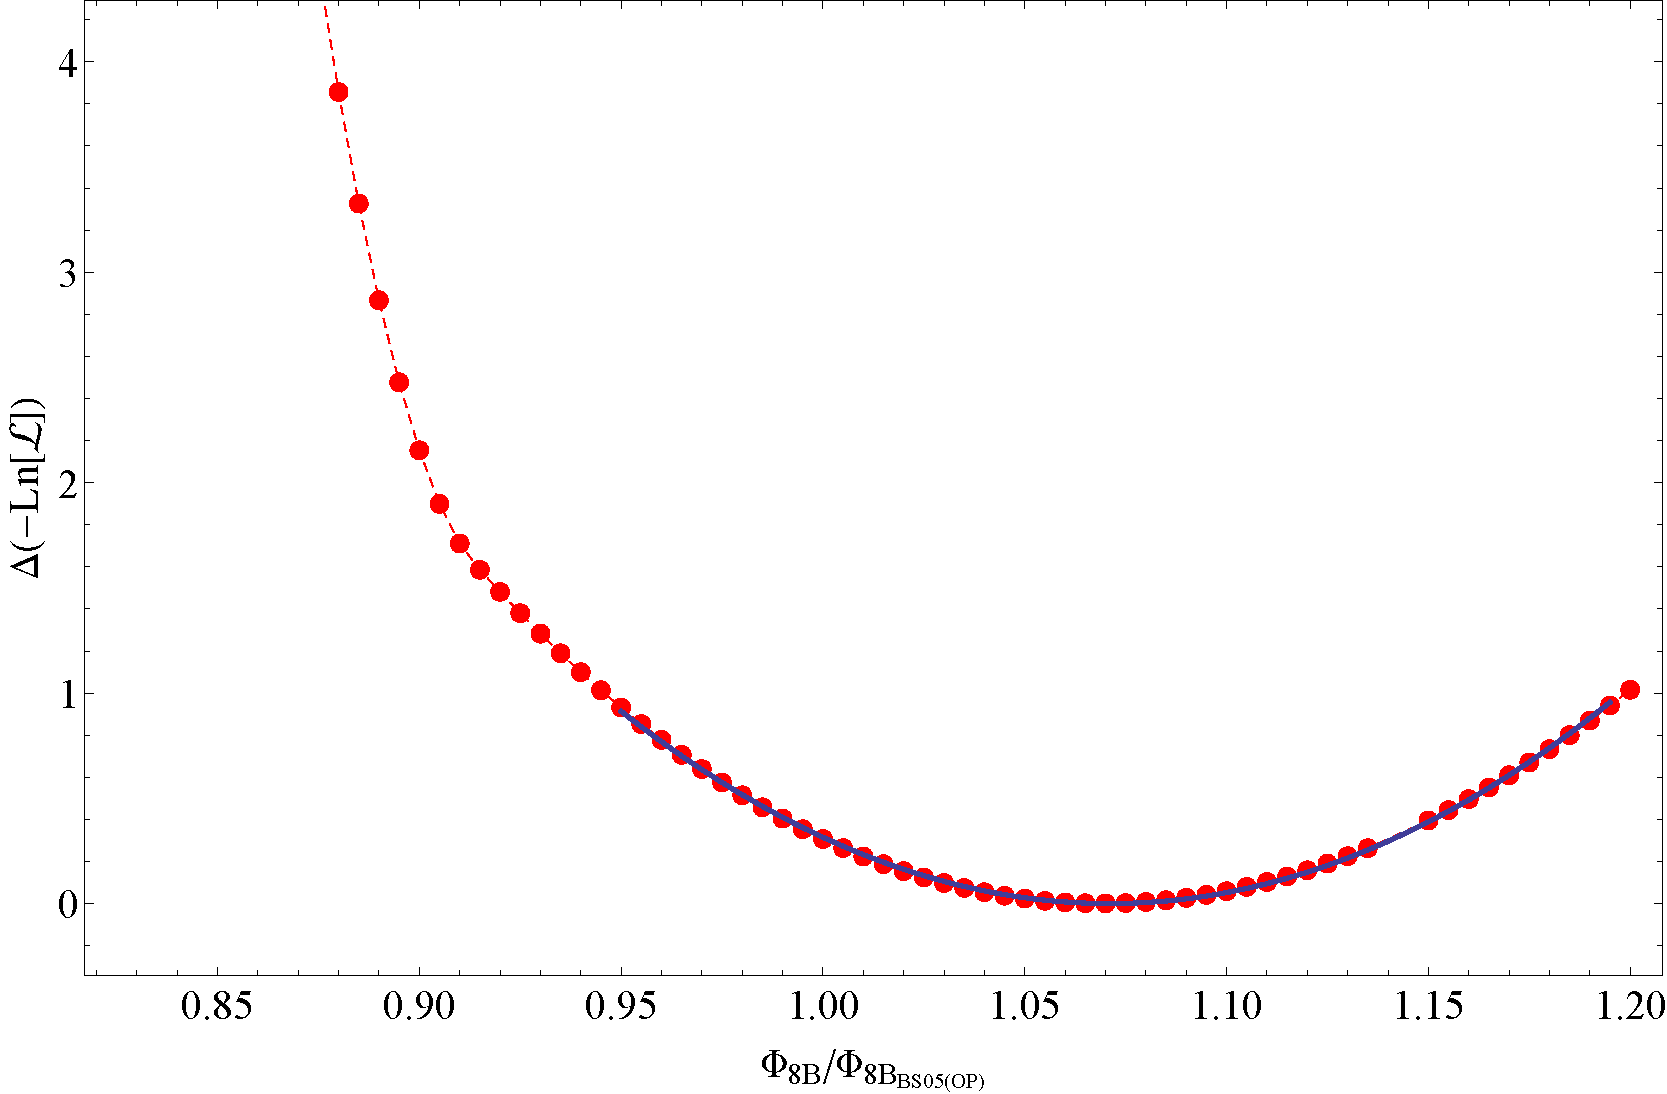
\includegraphics[width=0.85\columnwidth]{flux_scan_final}
\caption{The scans of $k_2$ and the $^8$B flux for the full dataset. The red points are the scan values, and the blue line is a fit to the minimum.}
\label{fig:final_scans}
\end{figure}

\begin{figure}
\centering
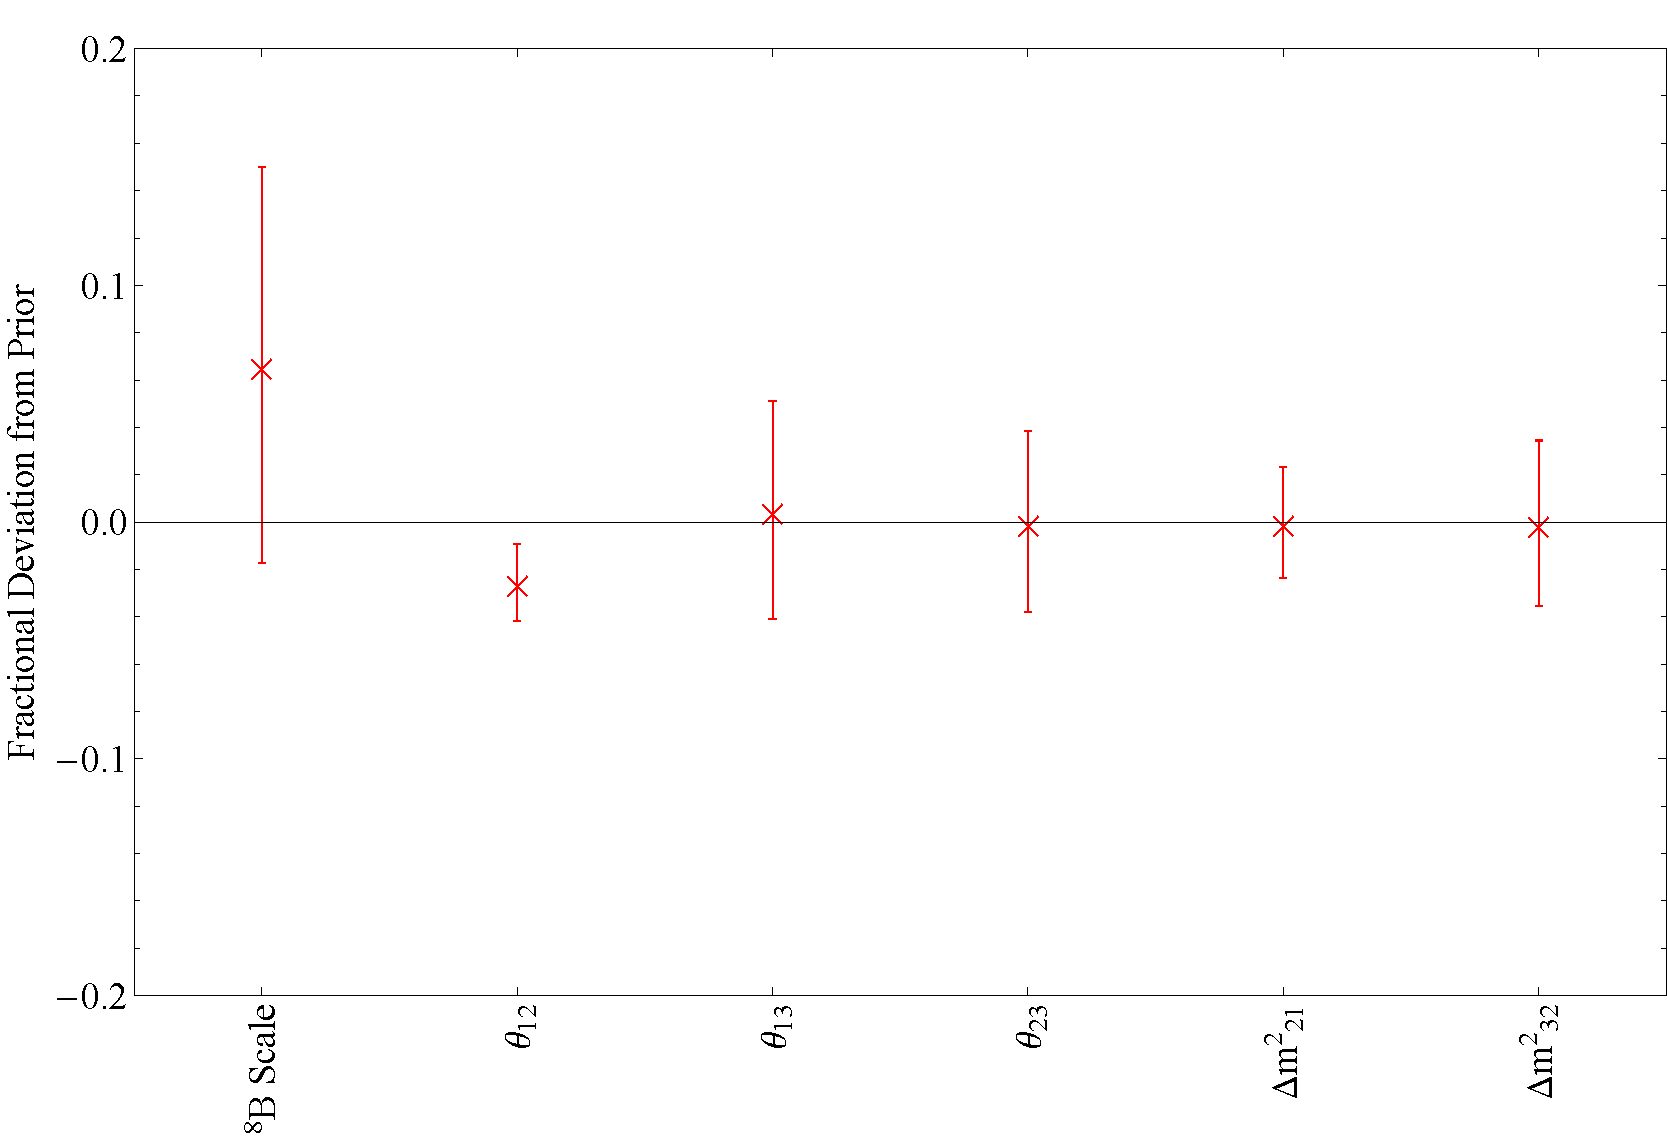
\includegraphics[width=0.85\columnwidth]{prior_deviation_final}
\caption{The fractional deviation of each neutrino parameter with a prior constraint from its prior. The errors shown are the fractional errors of the fit.}
\label{fig:priors_final}
\end{figure}

\begin{figure}
\centering
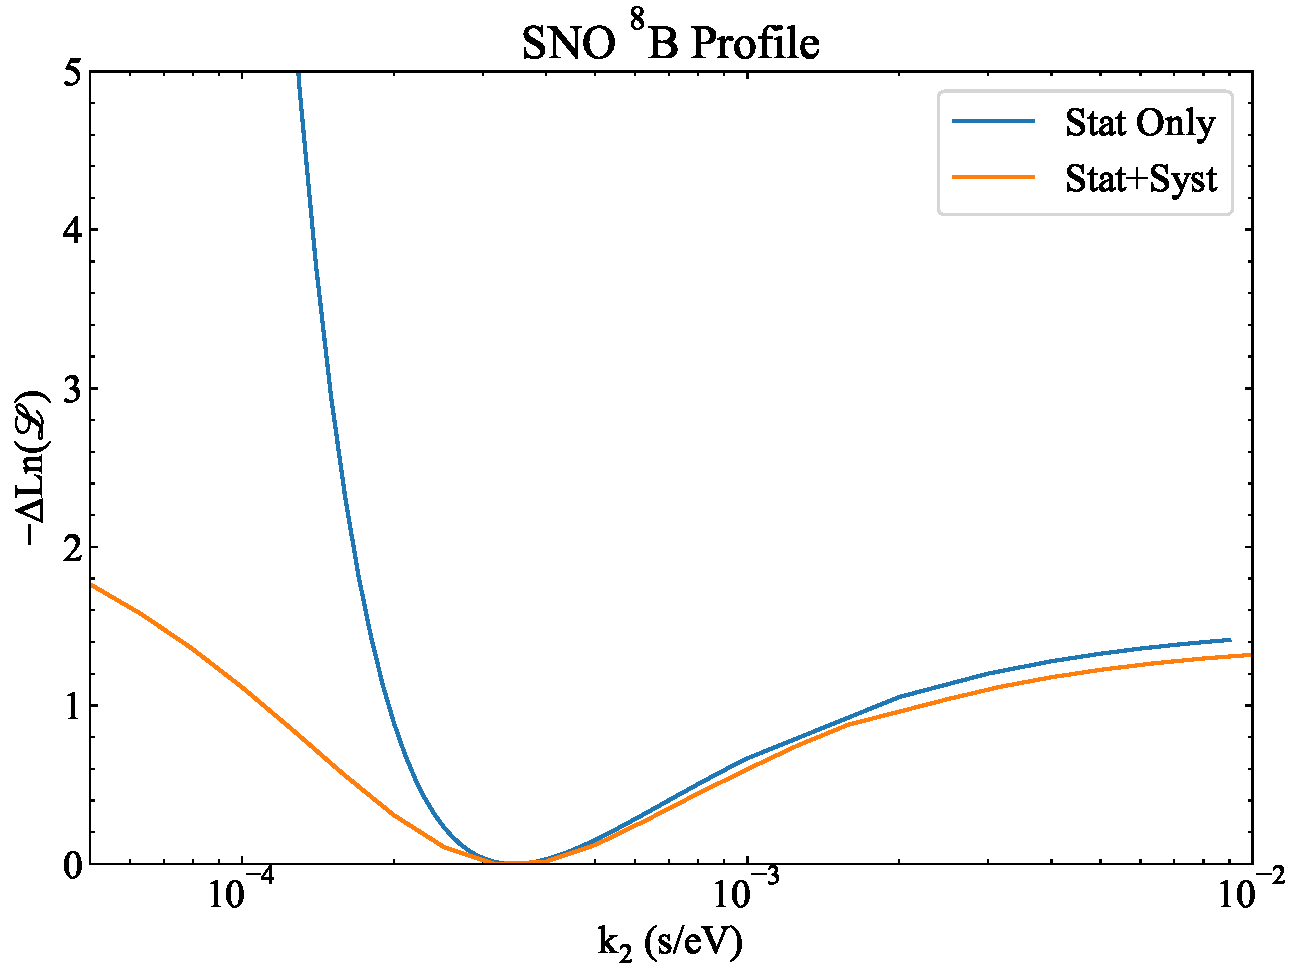
\includegraphics[width=0.85\columnwidth]{sno_8b_stat_syst_profile.pdf}
\caption{The scans of $k_2$ with and without systematic effects. Note that in both cases the minimum has been shifted to zero. With systematics included the minimum is less significant relative to the limiting value at $k_2 \rightarrow \infty$ as expected.}
\label{fig:systematic_scans}
\end{figure}

\clearpage

\section{Global Solar Neutrino Decay Analysis}

The SNO-only $90\%$ confidence lower bound at $>8.08\times10^{-5}$ s/eV from this analysis is not particularly competitive with the best combined analysis \cite{picoreti}, which sets a $99\%$ confidence lower bound at $>7.2\times10^{-4}$~s/eV (note order of magnitude).
This result was obtained by combining measurements from many solar experiments, and such an analysis can be repeated while including the SNO result described in previous sections.

Experiments have made measurements of solar neutrino interaction rates and published measured fluxes both assuming oscillations (a mixture of neutrino flavors) and no oscillations (assuming a pure electron neutrino flux). 
Practically, the oscillated fluxes are tricky to use because they always depend on a particular set of mixing parameters.
Fortunately, given an unoscillated flux of electron neutrinos, $\Phi_e$, it is straightforward to recover the true neutrino flux, $\Phi_T$ given some oscillation model and knowing the ratio of cross sections for electron $\sigma_e$ and other flavor $\sigma_a$ neutrinos.
\begin{equation}
\Phi_e = (P_{ee} + P_{ea} \frac{\sigma_a}{\sigma_e})\Phi_T
\label{flux_conv}
\end{equation}
The theory described in \Cref{lifetime_model} predicts a value for both $P_{ee}$ and $P_{ea}$ given a set of neutrino mixing parameters, a standard solar model, and a set of neutrino lifetimes.
Since the survival probabilities and cross sections are energy dependent, average quantities weighted by the detected energy spectrum are used.

The total neutrino flux inferred from the survival probability can be directly compared to a standard solar model flux $\Phi_{SSM}$ with a Gaussian constraint term:
\begin{equation}
\mathcal{L} = \frac{(\Phi_T - \Phi_{SSM})^2}{2 \sigma_\Phi^2}
\label{combolike}
\end{equation}
where $\sigma_\Phi$ combines the uncertainty from the measurement with the uncertainty from the SSM.
To account for uncertainties in mixing parameters, these are constrained with similar penalty terms by the same priors from the SNO lifetime analysis (see \Cref{lifetime_model}), and profiled out. 
The lifetime of mass state three is fixed at infinity (solar neutrino fluxes contain negligible amounts of mass state three), while the likelihood is minimized with respect to the lifetime of mass state one where appropriate.

\subsection{$^8$B Constraints}

SuperK~\cite{superkiv}, KamLAND~\cite{kamland8b} and Borexino~\cite{borexino8b} have all measured the $^8$B neutrino flux via the elastic scatter channel. 
For any particular set of neutrino parameters, the average survival probability values are computed for the elastic scatter cross section weighted energy spectrum of $^8$B neutrinos using the correct production regions (electron density) in the Sun. 
Using these survival probabilities, the measured $\Phi_e$ of each experiment is converted to a true $^8$B flux with \Cref{flux_conv} and compared to the SSM prediction with \Cref{combolike}.
To arrive at a profiled likelihood for each experiment, all neutrino parameters are floated with priors while scanning $k_2$. The lifetime of mass state one is fixed at infinity as with the SNO analysis. 
This produces the profiles in \Cref{fig:8b_profiles}.

\begin{figure}
\centering
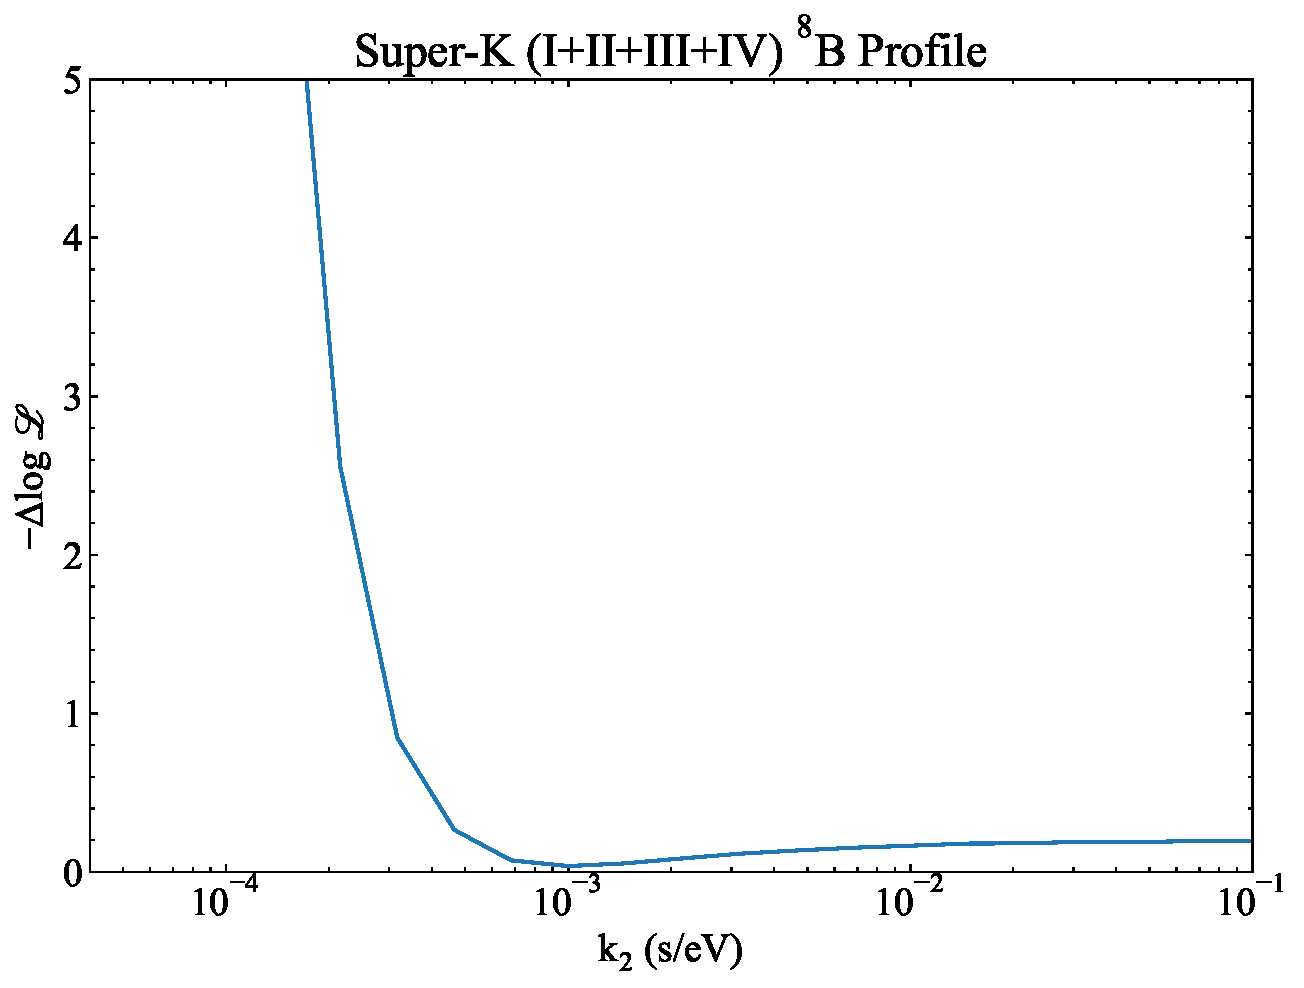
\includegraphics[width=0.5\columnwidth]{superk_8b}
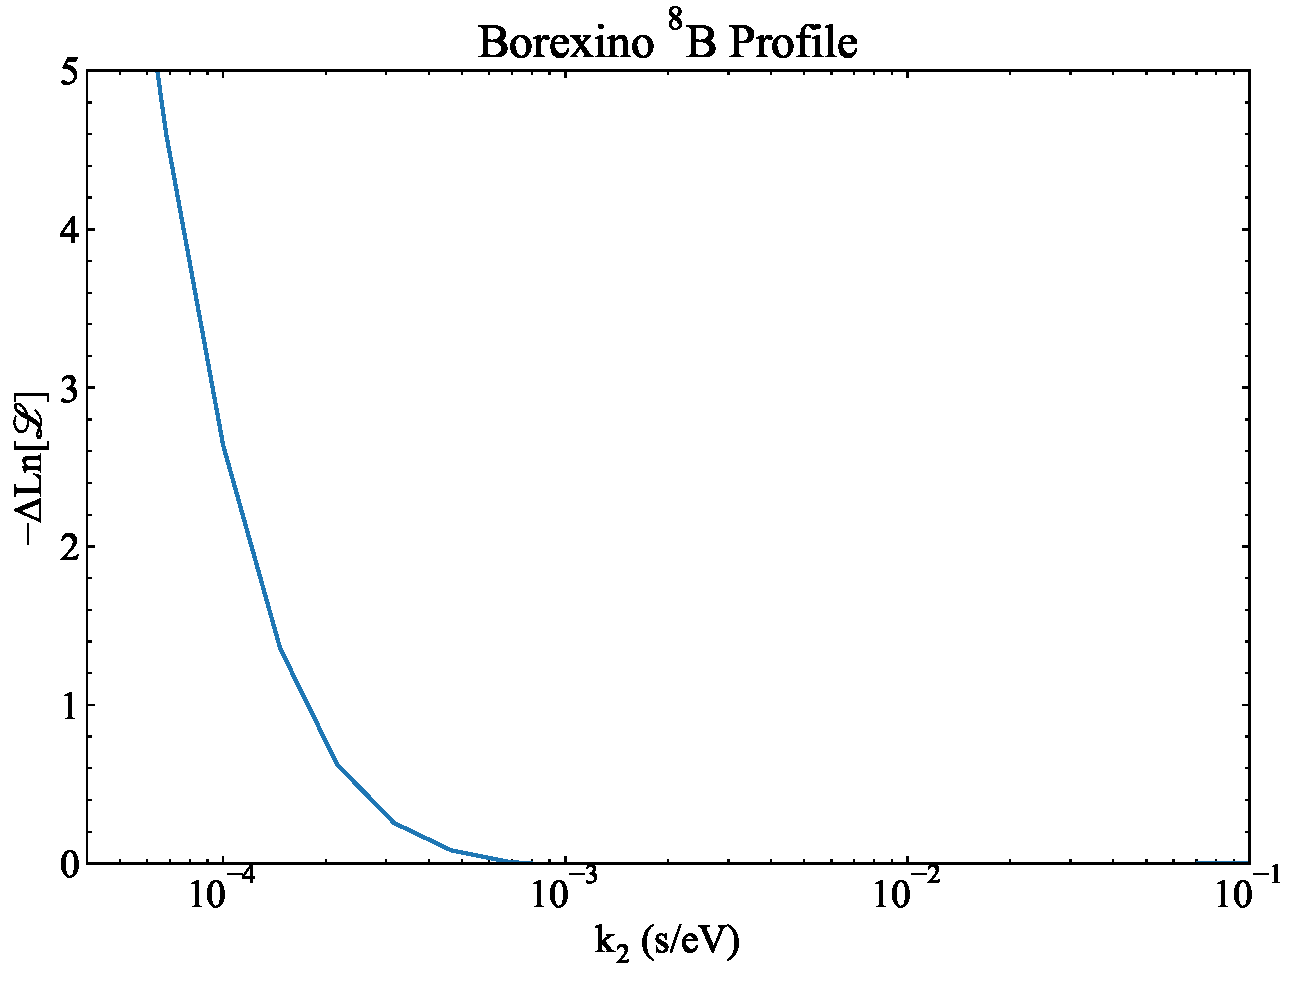
\includegraphics[width=0.5\columnwidth]{borexino_8b}
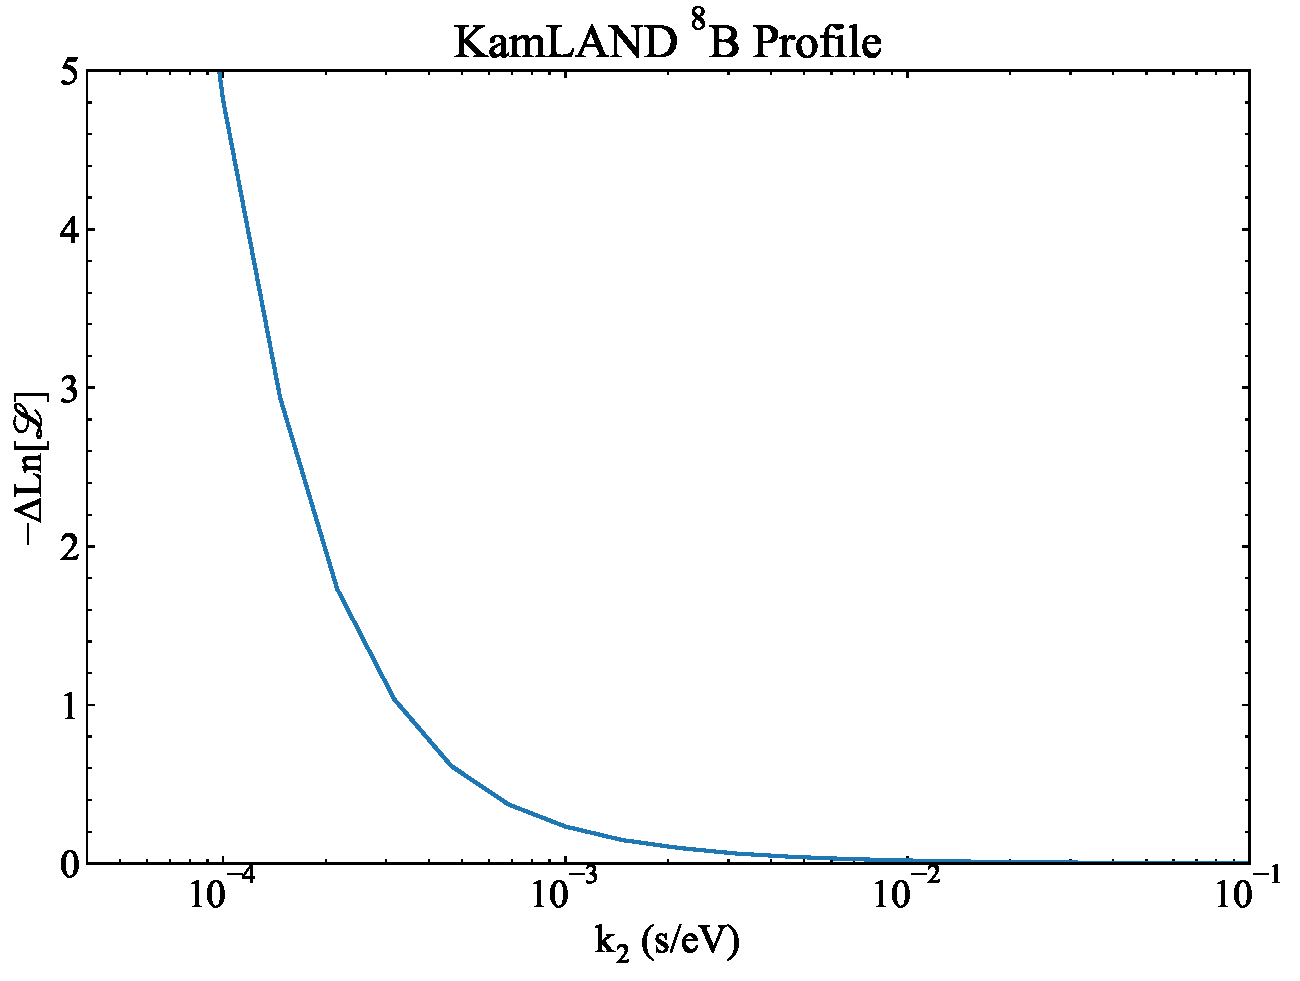
\includegraphics[width=0.5\columnwidth]{kamland_8b}
\caption{The profiled likelihood for the parameter $k_2$ using $^8$B measurements from SuperK~\cite{superkiv}, Borexino~\cite{borexino8b}, and KamLAND~\cite{kamland8b}.}
\label{fig:8b_profiles}
\end{figure}

\subsection{$^7$Be Constraints}

Borexino~\cite{borexino7be} and KamLAND~\cite{kamland7be} measured the 862~keV line of $^7$Be neutrinos, which account for $90\%$ of the flux from this isotope. 
The average survival probability weighted by the $^7$Be production regions for 862~keV neutrinos is computed for any particular set of neutrino parameters.
Using these survival probabilities, the measured $\Phi_e$ of each experiment is converted to a true $^7$Be flux with \Cref{flux_conv} and compared to the SSM prediction with \Cref{combolike}. 
As these neutrinos are much lower energy, they contain a significant fraction of mass state one. 
Here the lifetime of mass state one, $k_1$, is treated as a nuisance parameter and floated in the fit. 
The profiles in \Cref{fig:7be_profiles} are generated by scanning $k_2$ while floating neutrino parameters and $k_1$.

Note that these constraints are stronger than $^8$B constraints because these neutrinos are lower energy, so measured fluxes near the SSM prediction - even with less precision - can rule out shorter lifetimes.
This holds true (to some extent) for the radiochemical gallium and chlorine experiments discussed in the following sections.

\begin{figure}
\centering
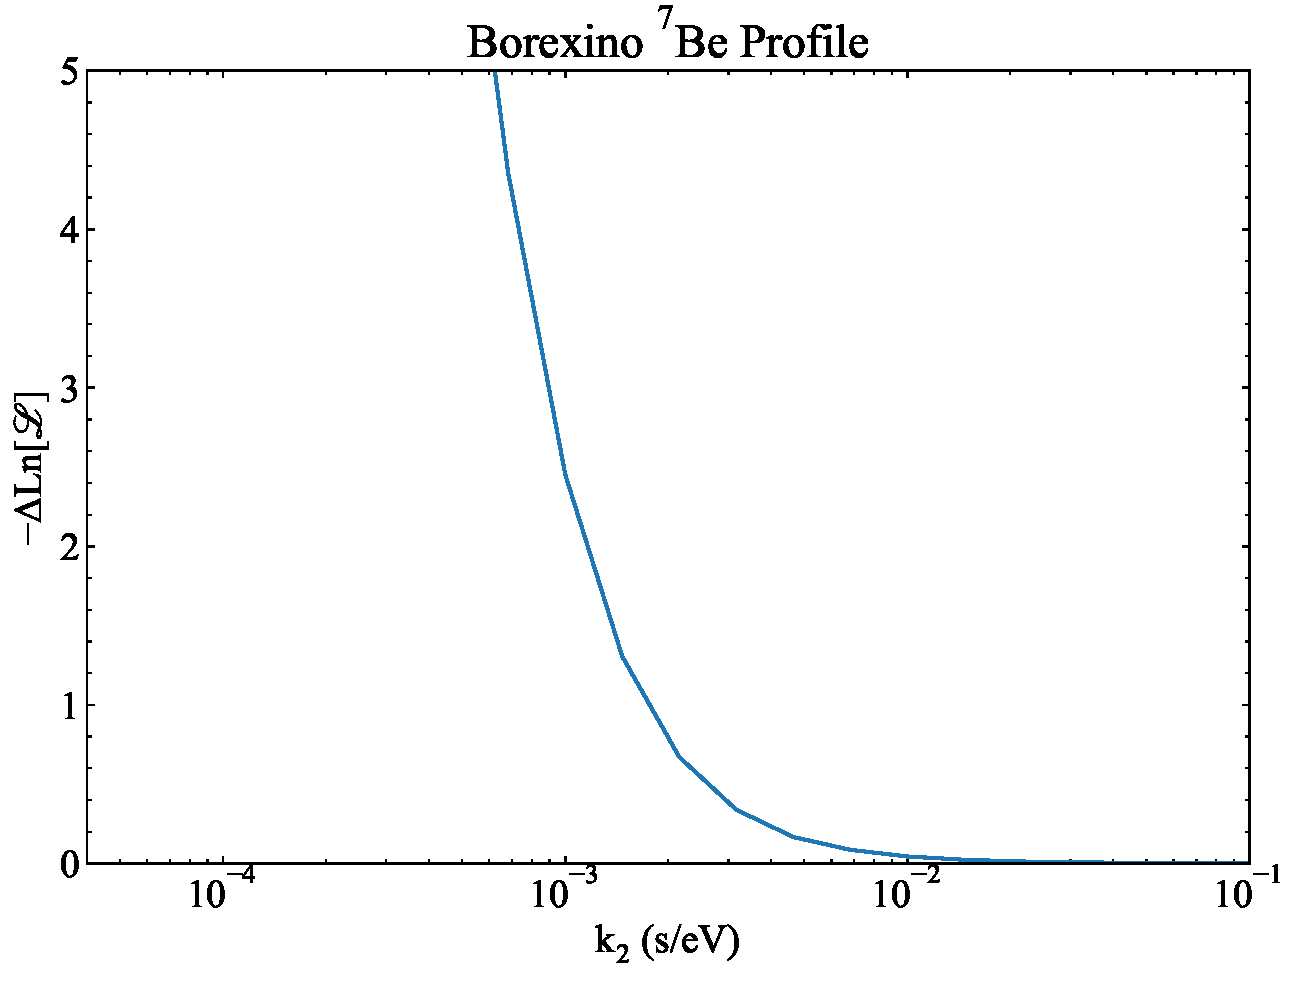
\includegraphics[width=0.58\columnwidth]{borexino_7be}
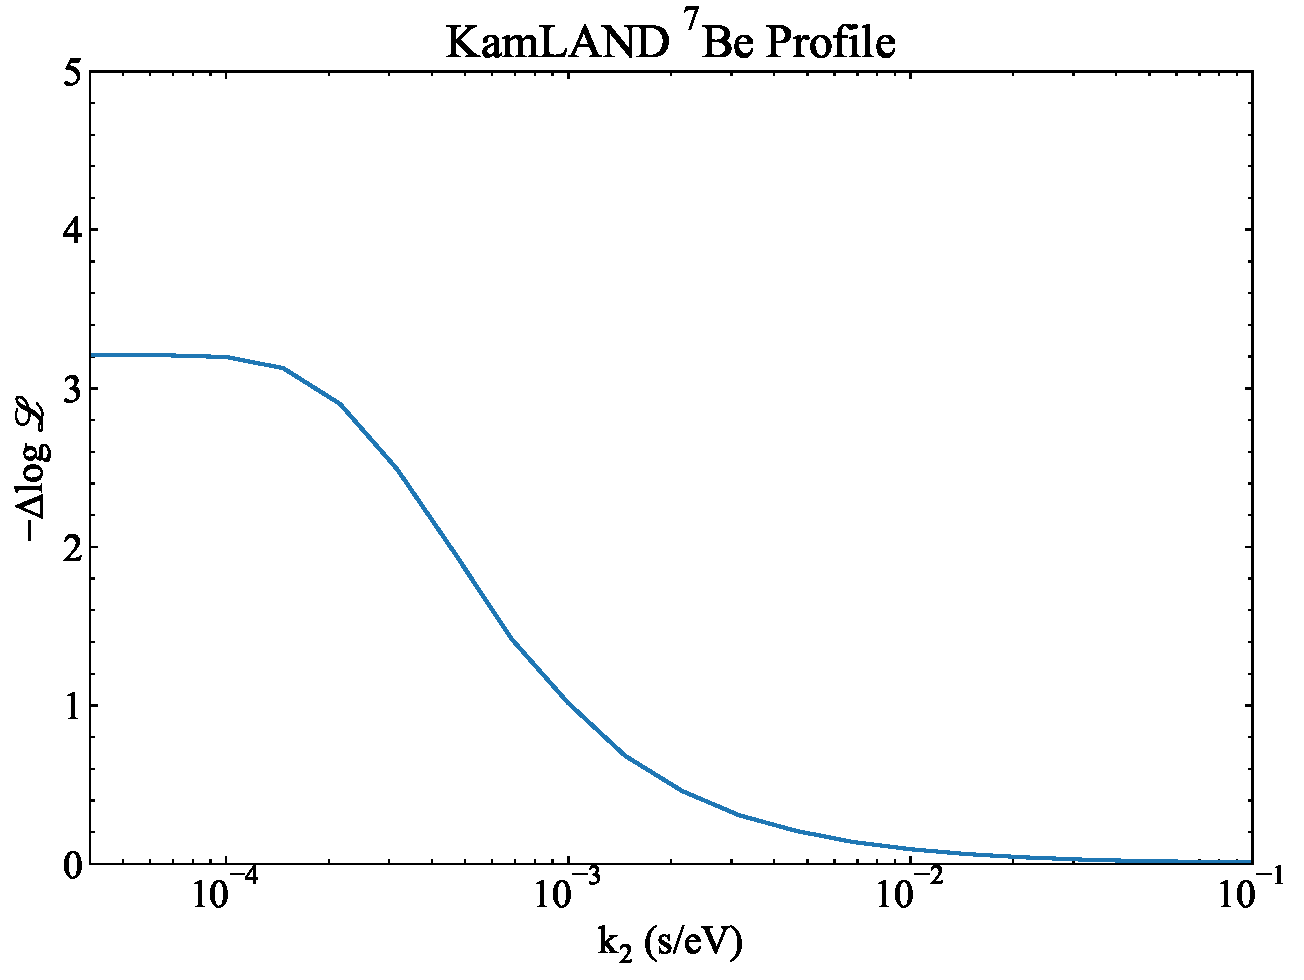
\includegraphics[width=0.58\columnwidth]{kamland_7be}
\caption{The profiled likelihood for the parameter $k_2$ using the $^7$Be 862~keV line measurements from Borexino~\cite{borexino7be} and KamLAND~\cite{kamland7be}. Note the shape of the Borexino profile is quite similar to KamLAND, however, the Borexino measurement excludes short lifetimes at higher significance due to being a more precise measurement.}
\label{fig:7be_profiles}
\end{figure}

\subsection{Gallium Constraints}

The SAGE~\cite{sagecombo} experiment has conveniently combined all gallium solar neutrino measurements into a single value: a rate of solar neutrino interactions on an atom of gallium. 
This requires a bit more effort than the $^8$B and $^7$Be measurements as this rate combines every type of solar neutrino flux, and is related to the fluxes by the gallium neutrino capture cross section.
It is most convenient to compute the expected interaction rate for a particular set of neutrino flux values and mixing parameters and compare this to the measured total rate. 
This follows the analysis described in Section V in \cite{sagecombo} with the notable exception that the survival probability used here includes neutrino decay.

For each type (that is, originating isotope) of solar neutrino, the average gallium cross section weighted by the energy spectrum and survival probability is calculated for a particular set of neutrino parameters using the appropriate production regions in the Sun for that type.
The gallium cross section used here is the same modified form used in the SAGE analysis~\cite{sagecombo}.
The sum of these average cross sections multiplied by the flux of each type yields the total interaction rate expected on gallium.
This quantity can be directly compared to the measured rate with a likelihood term similar to \Cref{combolike}.

A profiled likelihood is arrived at in a similar way as described above: neutrino parameters, SSM fluxes, and lifetime of mass state one are floated while $k_2$ is scanned. 
Neutrino parameters and SSM fluxes are constrained with the same priors as elsewhere in this analysis.
The result is shown in \Cref{fig:ga_profiles}.

\begin{figure}
\centering
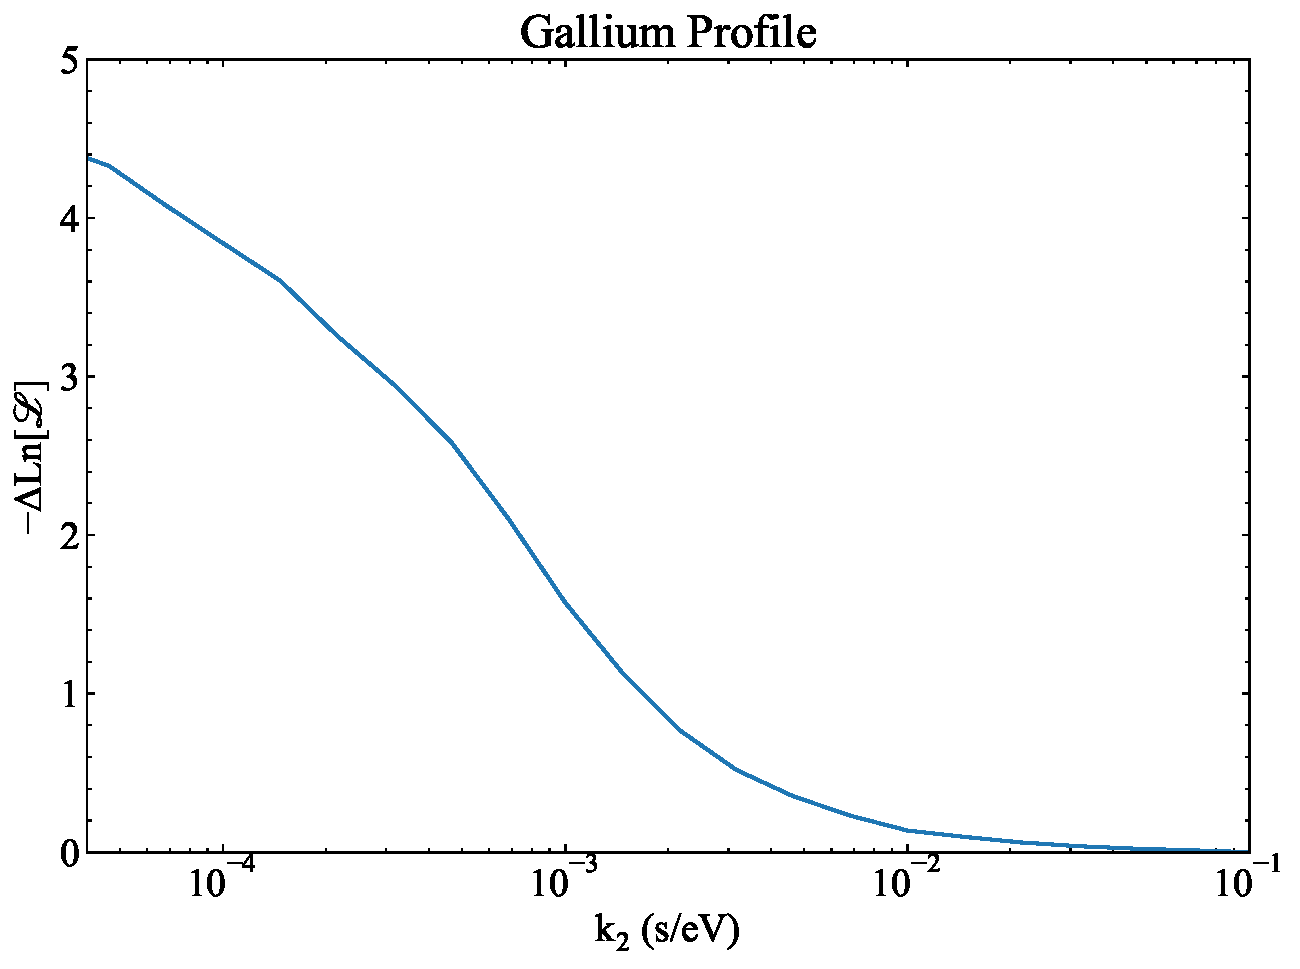
\includegraphics[width=0.58\columnwidth]{gallium_8b}
\caption{The profiled likelihood for the parameter $k_2$ using the combined measurement of all gallium experiments~\cite{sagecombo}.}
\label{fig:ga_profiles}
\end{figure}

\subsubsection{Validation}

As this is more complicated than a simple constraint, some additional verification is needed to ensure there are no issues with the code.
To that end I have reproduced the per-component interaction rate from Table IV of~\cite{sagecombo} in \Cref{tbl:gallium} using the mixing parameters and approximate form of the survival probability from that same reference.
As these values are nearly identical to those reported in the original publication, my calculation of cross sections and total rates appears consistent.

Note that~\cite{sagecombo} uses an approximate form of the survival probability whereas for all other parts of this analysis I have numerically diagonalized the MSW Hamiltonian (see \Cref{lifetime_model}).
A notable difference between these two approaches is that the approximate forms assume a uniform solar density for each flux, while my numerical method accounts for the density profile in the regions where these neutrinos originate.
Using my numerical computation instead of the approximate form yields slightly different numbers (also shown in \Cref{tbl:gallium}). 
Both total rates are consistent with the Gallium measurements $66.1\pm3.1$~SNU~\cite{sagecombo} at one sigma, and the numerical method is used for other parts of this analysis.

With the calculation of the expected rate validated, the remaining step of including gallium results in this analysis is a comparison to the measured rate with a term like \Cref{combolike}.

\begin{table}
\centering
\begin{tabular}{c|r|r|r}
Component & \cite{sagecombo} Rate (SNU) & Approximate $P_{ee}$ (SNU) & Numerical $P_{ee}$ (SNU) \\ \hline
$pp$		& 39.35	&	39.34 	&	39.18	\\
$pep$		& 1.43 	&	1.43 	&	1.35 	\\ 
$^7$Be		& 18.73	&	18.74	& 	18.78	\\
$^{13}$N	& 0.89 	&	0.89	&	0.85	\\ 
$^{15}$O	& 1.23 	&	1.23	&	1.13	\\ 
$^{17}$F	& 0.03 	&	0.03	&	0.03	\\
$^8$B		& 4.64 	&	4.63	&	4.54	\\ 
$hep$		& 0.02 	&	0.02	&	0.02	\\ \hline
Total		& 66.31	&	66.32 	&	65.80	\\ \hline
\end{tabular}
\caption{\label{tbl:gallium}Shown here are the predicted interaction rates of each neutrino flux with Gallium computed with the code developed for this analysis using both the approximate survival probability forms in~\cite{sagecombo} and the numerical forms used elsewhere in this analysis. Results from \cite{sagecombo} are reproduced for reference.}
\end{table}

\subsection{Chlorine Constraints}

The analysis of radiochemical measurements of interactions on chlorine is very similar to that of the gallium experiments described above. 
So, a similar analysis as done for gallium was performed here, but using the measured rate from the Homestake~\cite{homestake} experiment, $2.56\pm0.23$~SNU on $^{37}$Cl, along with the chlorine cross sections used for that analysis.
The result of the profile are found in in \Cref{fig:cl_profiles}.

\begin{figure}
\centering
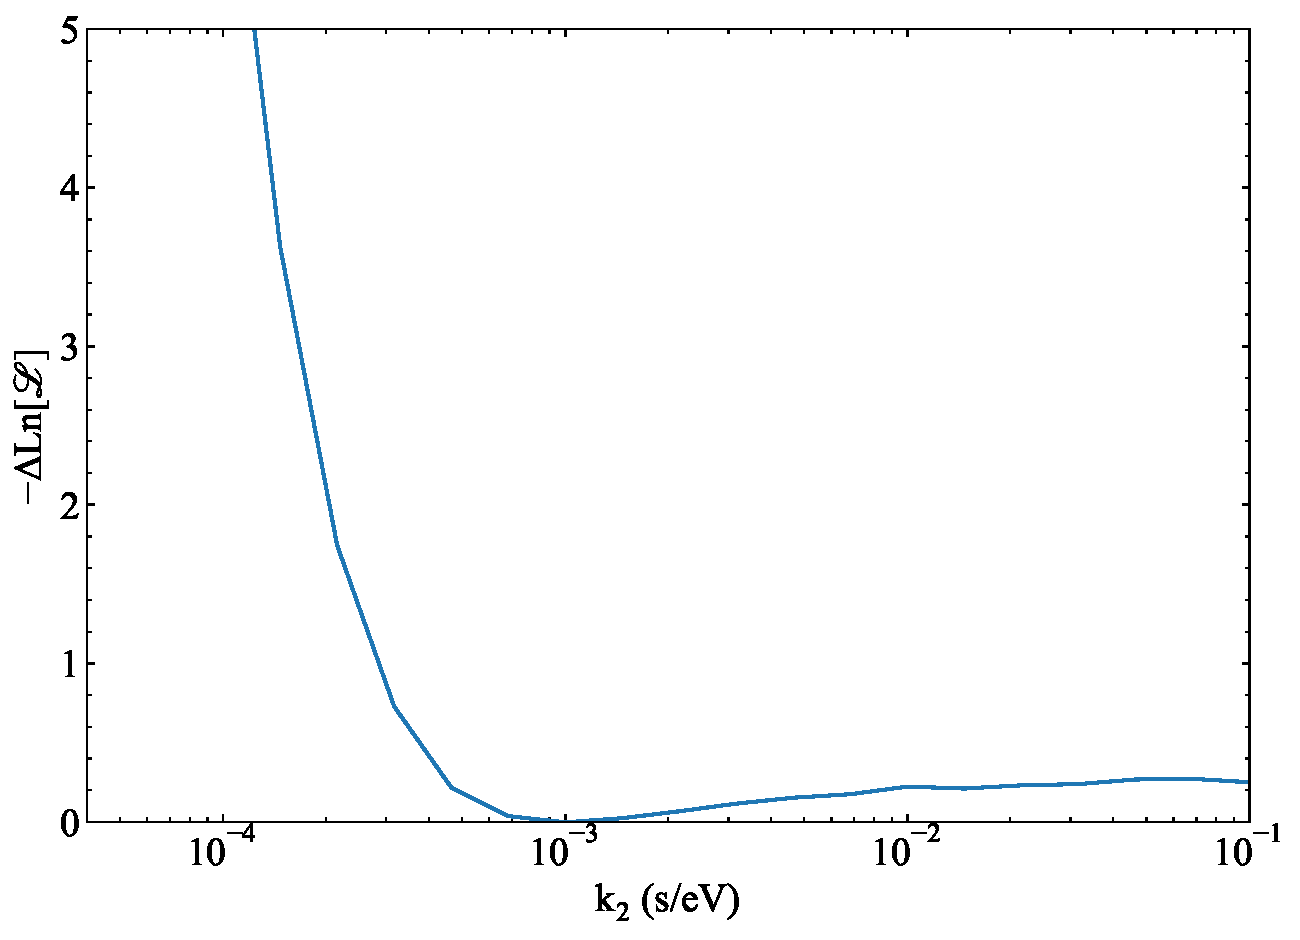
\includegraphics[width=0.58\columnwidth]{chlorine_8b}
\caption{The profiled likelihood for the parameter $k_2$ using the measurements from Homestake~\cite{homestake}.}
\label{fig:cl_profiles}
\end{figure}


\subsubsection{Validation}
The Homestake~\cite{homestake} experiment does not go into detail about expected rates from separate components.
Also, the references cited there tend to assume $P_{ee} = 1$ when calculating expected rates, which is not a useful comparison to make with this analysis.
A more recent paper~\cite{bachall_lma} does a modern calculation of the expected interaction rates per flux component that is directly comparable to the model used here.

Using the fluxes and mixing parameters quoted in Table I of \cite{bachall_lma}, I have reproduced the interaction rates central values for Chlorine in \Cref{tbl:chlorine} and compared to the LMA solution from Table I of \cite{bachall_lma}.
The column showing the `old' parameters are using the fluxes and mixing parameters from \cite{bachall_lma} while the column showing `new' parameters uses the SSM and mixing parameters used elsewhere in this analysis.
In all cases there is pretty good agreement with the measured rate from Homestake and between models.

\begin{table}
\centering
\begin{tabular}{c|r|r|r}
Component & \cite{bachall_lma} Rate (SNU) & `Old' Parameters (SNU) & `New' parameters (SNU) \\ \hline
$pp$		& 0.0	&	0.00 & 0.00		\\
$pep$		& 0.1 	&	0.13 & 0.12		\\ 
$^7$Be		& 0.46	&	0.45 & 0.30		\\
$^{13}$N	& 0.05 	&	0.05 & 0.02		\\ 
$^{15}$O	& 0.16 	&	0.17 & 0.07		\\ 
$^8$B		& 1.8 	&	1.82 & 2.20		\\ 
$hep$		& 0.1 	&	0.07 & 0.01		\\ \hline
Total		& 2.6	&	2.69 & 2.75		\\ \hline
\end{tabular}
\caption{\label{tbl:chlorine}Shown here are the predicted interaction rates of each neutrino flux with Chlorine both from an independent calculation \cite{bachall_lma}, using this analysis' code with the `old' mixing and flux parameters in that reference, and again with the flux and mixing parameters used elsewhere in this analysis.}
\end{table}

\subsection{Combined Result}
\label{sec:combobreaker}

The likelihood profiles of individual experiments are multiplied (negative log likelihoods added) together to arrive at a combined likelihood profile shown in \Cref{fig:combined_profile}. 
Explicitly this includes: $^8$B measurements from KamLAND, Borexino, SuperK (I,II,III,IV) and this analysis of SNO data, $^7$Be measurements from KamLAND and Borexino, and total rate measurements from all gallium experiments (SAGE+GNO+GALLEX) plus the Homestake results on chlorine. 
The $99\%$ C.L. lower bound for the lifetime of mass state two is $>10.41\times10^{-4}$~s/eV. 
This is better than the previous analysis for a few reasons: KamLAND results were not previously included, and both Borexino and Super-K published updated analyses compared to the data used in the previous limit. 
Notably the presence of a relatively significant minimum in the new SNO results is not particularly beneficial here since it occurs near the location of the limit.

\subsection{Cross-Check with Previous Limit}

The analysis that set the best limit~\cite{picoreti} did not go into detail as to how their analysis was performed, or which SSM values were used as a reference.
This makes it difficult to precisely reproduce their results, however, since they do list the experimental results used, I can repeat my analysis using those experimental results and see if I get a similar limit.

The experiments used in the previous best limit were: Homestake (Cl), Sage (Ga), GNO+GALLEX (Ga), Borexino's first $^7$Be publication, SNO's 3-phase analysis, and Super-K (I). 
Homestake and the gallium experiments have not been updated and are handled as described above.
Borexino and Super-K (I) are handled as described above but with the less-precise flux determinations of those two analyses. 
The SNO 3-phase results are handled in an analogous way to Super-K results using only the flux information.


In \Cref{fig:cross_check_profile} I have combined the profiles from these measurements and arrived at a limit of $>7.58\times10^{-4}$~s/eV at $99\%$ C.L., a bit better than \cite{picoreti}'s quoted $>7.2\times10^{-4}$~s/eV at $99\%$ C.L..
That this is quite close to the limit set by~\cite{picoreti} indicates that these two analyses are consistent even if the methods presumably differ.
Unfortunately with the brevity of the previous paper a more direct comparison does not seem possible.

\begin{figure}
\centering
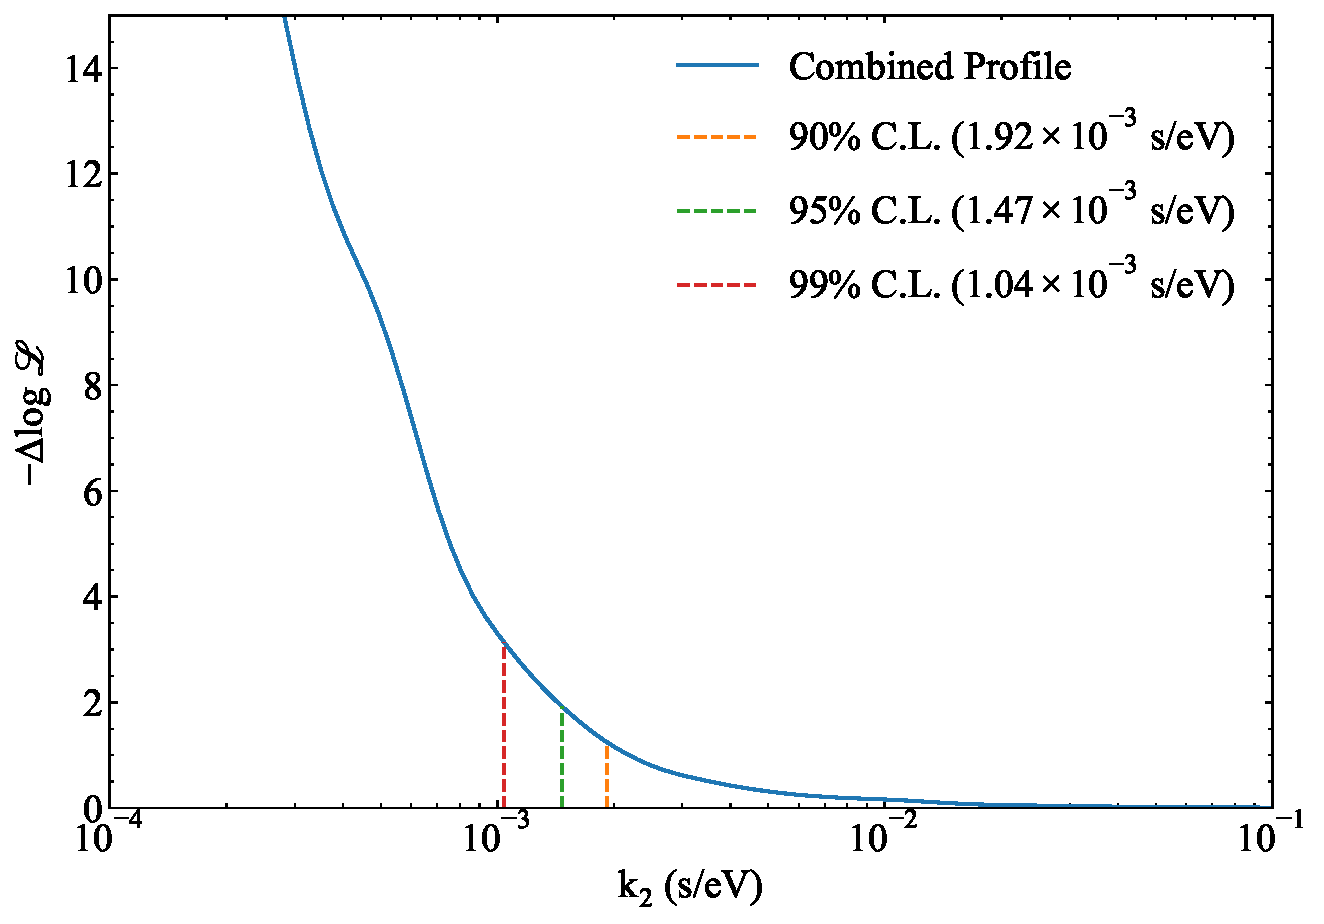
\includegraphics[width=0.85\columnwidth]{combined_profile}
\caption{The combined profiled likelihood described in \Cref{sec:combobreaker}.}
\label{fig:combined_profile}
\end{figure}

\begin{figure}
\centering
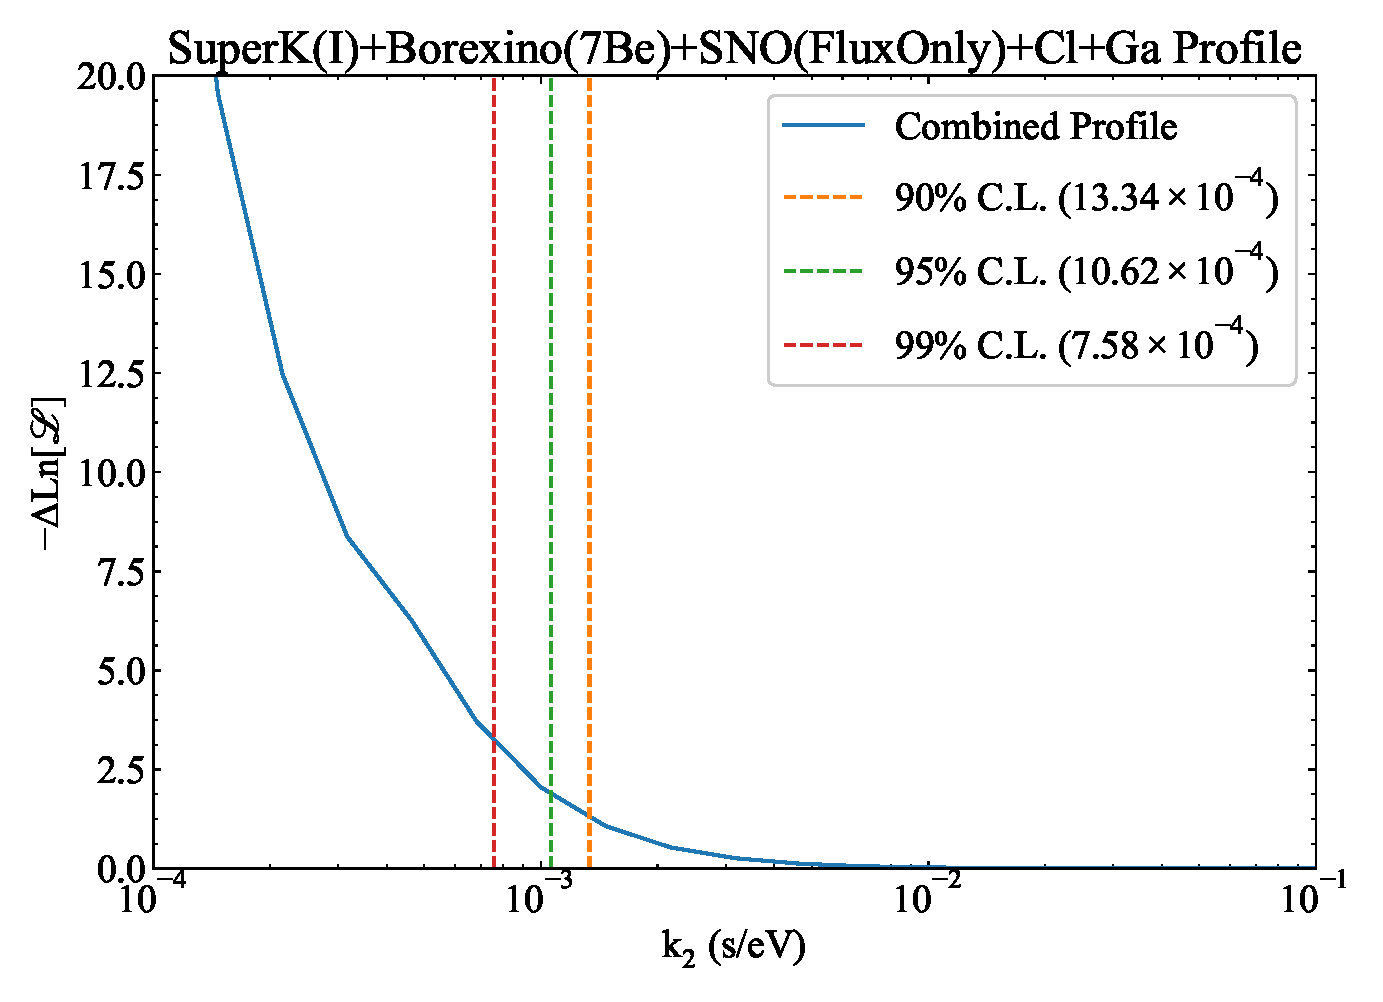
\includegraphics[width=0.85\columnwidth]{cross_check_profile}
\caption{The combined profile intended to reproduce the result in \cite{picoreti} by using the same experimental measurements. Notably the analysis methods are not identical so the results should be similar but do not match exactly.}
\label{fig:cross_check_profile}
\end{figure}
